\documentclass[12pt,spanish,fleqn,openany,letterpaper,pagesize]{scrbook} %report, scrbook

\usepackage[ansinew]{inputenc}
\usepackage[english]{babel}
\usepackage{dingbat}
\usepackage{fancyhdr}
\usepackage{epsfig}
\usepackage{epic}
\usepackage{eepic}
\usepackage{amsmath}
\usepackage{threeparttable}
\usepackage{amscd}
\usepackage{here}
\usepackage{graphicx}
\usepackage{lscape}
\usepackage{tabularx}
\usepackage{subfigure}
\usepackage{longtable}
\usepackage{tabularx,colortbl}
\usepackage{color}
\usepackage{xcolor}

\usepackage{titlesec}
\setcounter{tocdepth}{3}
\setcounter{secnumdepth}{3}

%tables
\usepackage{pbox}
\usepackage{longtable} % para tablas largas
\usepackage{lipsum}
\usepackage{ragged2e}
% centering cells
\newcolumntype{P}[1]{>{\centering\arraybackslash}p{#1}}
%Numbers with circle:
\usepackage{tikz}
\newcommand*\circled[1]{\tikz[baseline=(char.base)]{
            \node[shape=circle,draw,inner sep=2pt] (char) {#1};}}

%algorithm2e and comment style
\usepackage[ruled,vlined,linesnumbered]{algorithm2e}
\newenvironment{english_algorithm}[1][htb]
  {\renewcommand{\algorithmcfname}{Algorithm}% Update algorithm name
   \begin{algorithm}[#1]%
  }{\end{algorithm}}

%///////////////////////////////////
%\usepackage[utf8]{inputenc}
% Hyper-references
\usepackage[unicode=true, bookmarks=true,bookmarksnumbered=true,bookmarksopen=false, breaklinks=true, pdfborder={0 0 0},backref=page,colorlinks=true]{hyperref}
\hypersetup{pdftitle={Master Dissertation Intelligent Probing for SDN Monitoring}, pdfauthor={Edwin Ferney Castillo Quintero}, colorlinks=true, citecolor=blue,linkcolor=black, urlcolor=green}

\usepackage{rotating} %Para rotar texto, objetos y tablas seite. No se ve en DVI solo en PS. Seite 328 Hundebuch
                        %se usa junto con \rotate, \sidewidestable ....

\usepackage{svg}

\renewcommand{\theequation}{\thechapter-\arabic{equation}}
\renewcommand{\thefigure}{\textbf{\thechapter-\arabic{figure}}}
\renewcommand{\thetable}{\textbf{\thechapter-\arabic{table}}}


\pagestyle{fancyplain}%\addtolength{\headwidth}{\marginparwidth}

%color linea del header
%\renewcommand{\headrulewidth}{2pt}% 2pt header rule
%\renewcommand{\headrule}{\hbox to\headwidth{%
%  \color{red}\leaders\hrule height \headrulewidth\hfill}}

%\oddsidemarginDenota el margen izquierdo de una p ́agina impar
%.\evensidemarginDenota el margen izquierdo en una p ́agina par
%http://ima.udg.es/Docencia/3105200736/tema9p.pdf
%\textheight22.5cm \topmargin0cm \textwidth16.5cm
\textheight22.0cm \topmargin0cm \textwidth16.5cm
\oddsidemargin0.5cm \evensidemargin-0.5cm%

\renewcommand{\chaptermark}[1]{\markboth{\thechapter\; #1}{}}
\renewcommand{\sectionmark}[1]{\markright{\thesection\; #1}}

\lhead[\fancyplain{}{\thepage}]{\fancyplain{}{\rightmark}}
\rhead[\fancyplain{}{\leftmark}]{\fancyplain{}{\thepage}}
\fancyfoot{}
\thispagestyle{fancy}%



\addtolength{\headwidth}{0cm}
\unitlength1mm %Define la unidad LE para Figuras
\mathindent0cm %Define la distancia de las formulas al texto,  fleqn las descentra
\marginparwidth0cm
\parindent0cm %Define la distancia de la primera linea de un parrafo a la margen

%Para tablas,  redefine el backschlash en tablas donde se define la posici\'{o}n del texto en las
%casillas (con \centering \raggedright o \raggedleft)
\newcommand{\PreserveBackslash}[1]{\let\temp=\\#1\let\\=\temp}
\let\PBS=\PreserveBackslash

%Espacio entre lineas
\renewcommand{\baselinestretch}{1.1}

%Neuer Befehl f\"{u}r die Tabelle Eigenschaften der Aktivkohlen
\newcommand{\arr}[1]{\raisebox{1.5ex}[0cm][0cm]{#1}}

%Neue Kommandos
\usepackage{Befehle}


%Trennungsliste
\hyphenation {Q-learning swit-ches}

\usepackage{pbsi}
\usepackage[T1]{fontenc}

\usepackage{datetime}
\newdateformat{monthyeardate}{%
  \monthname[\THEMONTH] \THEYEAR}

\newdateformat{yeardateonly}{%
  \yearname \THEYEAR} 
  
%Command             10pt    11pt    12pt
%\tiny               5       6       6
%\scriptsize         7       8       8
%\footnotesize       8       9       10
%\small              9       10      10.95
%\normalsize         10      10.95   12
%\large              12      12      14.4
%\Large              14.4    14.4    17.28
%\LARGE              17.28   17.28   20.74
%\huge               20.74   20.74   24.88
%\Huge               24.88   24.88   24.88

%enumerate list with circle
\newcommand*\circled[1]{\kern-2.5em%
  \put(0,4){\color{blue}\circle*{18}}\put(0,4){\circle{16}}%
  \put(-3,0){\color{white}\bfseries\large#1}~~}
\usepackage{enumitem}

%Including pages from PDF documents - https://texblog.org/2011/10/26/including-pages-from-pdf-documents/
\usepackage{pdfpages}

%\includeonly{Kap1/Kap1,Kap2/Kap2}
\begin{document}
%\maketitle
\pagenumbering{roman}
%\newpage
%\setcounter{page}{1}
\begin{center}
    \thispagestyle{empty} \vspace*{-0.5cm} \textbf{\huge
        Intelligent Probing for SDN Monitoring}\\[2.0cm]
    \begin{figure}[h!]
        \centering%
        
\includegraphics[scale=0.45]{CoverSheet/logo_unicauca}
    \end{figure}~\\[1.0cm]
    \Large\textbf{Edwin Ferney Castillo Quintero}\\[1.5cm]
    \Large \fontfamily{ptm}\selectfont {Dissertation of Master in Telematics Engineering \par} ~\\[2.0cm]
    \normalsize \fontfamily{ptm}\selectfont {Advisor:\\ Ph.D. Oscar Mauricio Caicedo Rendon \par} ~\\[2.5cm]
    \Large \bsifamily {Universidad del Cauca \par}
    \normalsize \fontfamily{ptm}\selectfont {Faculty of Electronic and Telecommunications Engineering \par}
    \normalsize \fontfamily{ptm}\selectfont {Department of Telematics \par}
    \normalsize \fontfamily{ptm}\selectfont {Line of Research in Advanced Services of Telecommunications \par}
    \normalsize \fontfamily{ptm}\selectfont {Popay\'an, \monthyeardate\today \par}
\end{center}

\newpage{\pagestyle{empty}\cleardoublepage}

\newpage
\begin{center}
\Large\textbf{Edwin Ferney Castillo Quintero} ~\\[5.0cm]
\thispagestyle{empty} \vspace*{0cm} \textbf{\huge
    \Large Intelligent Probing for SDN Monitoring} ~\\[3.0cm]

    \normalsize {A dissertation submitted to the Faculty of Electronic and Telecommunications Engineering of the Universidad del Cauca for the Degree of:} ~\\[1.5cm]
    \normalsize \textbf{Master in Telematics Engineering} ~\\[3.0cm]
    \normalsize \fontfamily{ptm}\selectfont {Advisor: ~\\ Oscar Mauricio Caicedo Rendon ~\\ Ph.D. in Computer Science} ~\\[3.0cm]
    %\normalsize \fontfamily{ptm}\selectfont {Popay\'an, \yeardateonly\today}
    \normalsize \fontfamily{ptm}\selectfont {Popay\'an, \monthyeardate\today \par}
\end{center}

\newpage{\pagestyle{empty}\cleardoublepage}

\newpage
\thispagestyle{empty} \textbf{}\normalsize
\\\\\\%
%\textbf{(Dedicatoria o un lema)}\\[4.0cm]

\begin{flushright}
\begin{minipage}{8cm}
    \noindent
        \small
        \textit{I've been a fortunate man in life, nothing has come easy.\\\\
        Sigmund Freud\\
        }
\end{minipage}
\end{flushright}

\newpage{\pagestyle{empty}\cleardoublepage}
\newpage
\thispagestyle{empty} \textbf{}\normalsize
\\\\\\%
\textbf{\LARGE Acknowledgment}\\\\

Acknowledgments are written in Spanish because of my family. Ha sido un largo camino hasta llegar a este punto. Quiero aprovechar estas l\'ineas para agradecer a todas las personas que me han acompa\~nado, en los buenos y en los malos momentos, a lo largo de mi etapa universitaria y cuyo desenlace tiene lugar con este trabajo de Maestr\'ia\\

A mis padres, Graciela Quintero y \'Alvaro Castillo por su apoyo incondicional, por sus consejos, por su cari\~no, por sus valores y por ser todos ellos grandes ejemplos de perseverancia y animarme a seguir hacia delante en cada etapa de mi vida; su dedicaci\'on y sacrificio han sido la base para mi progreso. \\

A mis hermanos, no solo por estar presentes aportando buenas cosas a mi vida, sino por los grandes momentos de felicidad y de diversas emociones que siempre me han causado. A mi hermano Albert por ser mi inspiraci\'on y motivante para mejorar d\'ia a d\'ia.\\

A m\'i querida esposa Esledin por su apoyo incondicional, por sus consejos, por su amor, por siempre estar ah\'i; sin ti lograrlo hubiese sido m\'as dif\'icil. A mis dos grandes tesoros Jos\'e y Tefy, el mejor regalo que haya podido recibir de parte de Dios; gracias a ellos por ser la felicidad de mi vida.\\

A mis amigos, a los de toda la vida y a todos aquellos que he tenido el placer de conocer durante la carrera y la Maestr\'ia. Porque sin ustedes estos a\~nos no tendr\'ian el significado que han tenido para m\'i. Gracias por todo el apoyo y por los buenos momentos que hemos compartido y que seguiremos compartiendo.\\

Y, por supuesto, a mi tutor PhD Oscar Mauricio Caicedo Rend\'on. Porque sin \'el no habr\'ia sido posible la realizaci\'on de este trabajo. Me gustar\'ia destacar su apoyo, porque siempre han estado ah\'i cuando lo he necesitado. Adem\'as siempre me ha proporcionado invaluables consejos y se ha preocupado por que se hicieran las cosas de la mejor forma posible. Indudablemente por su influencia hoy soy mejor persona, mejor padre y mejor investigador.


\newpage{\pagestyle{empty}\cleardoublepage}
\newpage
\thispagestyle{empty} \textbf{}\normalsize
\\\\\\%
\textbf{\LARGE Abstract}\\\\
%\addcontentsline{toc}{chapter}{Abstract}\\\\
Traffic Monitoring assists in achieving the stability of networks by observing and quantifying their behavior. A proper traffic monitoring solution requires the accurate and timely collection of flow statistics. Many approaches have been proposed to monitor Software-Defined Networks. However, these approaches have diverse shortcomings. First, they are unconcerned about the trade-off between the probing interval and the Monitoring Accuracy (MA). Second, they lack intelligent mechanisms intended to optimize this trade-off by learning from network behavior. This master dissertation introduces an approach, called IPro, to address these shortcomings. IPro is formed by an architecture that follows the Knowledge-Defined Networking paradigm, an algorithm based on Reinforcement Learning, and an IPro prototype. In particular, IPro uses Reinforcement Learning to determine the probing interval that keeps within thresholds (target values) the Control Channel Overhead (CCO) and the Extra CPU Usage of the Controller (CUC). An extensive quantitative evaluation corroborates that IPro is an efficient approach for SDN Monitoring regarding CCO, CCU, and MA.\\[2.0cm]


\textbf{\small Keywords: Knowledge-Defined Networking, Machine Learning, Probing Interval, Software-Defined Networking, Traffic Monitoring}\\
\newpage
\textbf{\LARGE Resumen}\\\\
%\addcontentsline{toc}{chapter}{Abstract}\\\\
La monitorizaci\'on de tr\'afico ayuda a lograr la estabilidad de las redes al observar y cuantificar su comportamiento. Una soluci\'on de monitorizaci\'on de tr\'afico adecuada requiere la recopilaci\'on precisa y oportuna de estad\'isticas de flujo. Diversos investigadores han propuesto multiples enfoques para monitorear Redes Definidas por Software (Software-Defined Networks - SDN). Sin embargo, estos enfoques tienen algunas deficiencias. En primer lugar, no les preocupa el balance entre el intervalo de sondeo y la precisi\'on de monitoreo (Monitoring Accuracy - MA). En segundo lugar, carecen de mecanismos inteligentes destinados a optimizar este balance al aprender del comportamiento de la red. Esta disertaci\'on de maestr\'ia introduce un enfoque, llamado IPro, para abordar estas deficiencias. IPro est\'a formado por una arquitectura que sigue el paradigma de las Redes Definidas por el Conocimiento (Knowledge-Defined Networking - KDN), un algoritmo basado en el Aprendizaje por Refuerzo (Reinforcement Learning - RL) y un prototipo de IPro. En particular, IPro utiliza RL para determinar el intervalo de sondeo que mantiene dentro de umbrales (valores objetivo) la sobrecarga del canal de control (Control Channel Overhead - CCO) y el uso adicional de la CPU del controlador (CPU Usage of the Controller - CUC). Una extensa evaluaci\'on cuantitativa corrobora que IPro es un enfoque eficiente para el monitoreo de SDN con respecto a CCO, CCU y MA. \\ [2.0cm]


\thispagestyle{empty} \textbf{}\normalsize

\renewcommand{\tablename}{\textbf{Table}}
\renewcommand{\figurename}{\textbf{Figure}}
\renewcommand{\listtablename}{List of Tables}
\renewcommand{\listfigurename}{List of Figures}
\newcommand{\listbbreviaturename}{List of abbreviations and Acronyms}
\renewcommand{\contentsname}{Content}

\newpage{\pagestyle{empty}\cleardoublepage}
\newpage

%\newcommand{\clearemptydoublepage}{\newpage{\pagestyle{empty}\cleardoublepage}}
\tableofcontents
%\listoftables
\newpage{\pagestyle{empty}\cleardoublepage}
\newpage

\chapter*{List of Abbreviations and Acronyms}
\addcontentsline{toc}{chapter}{\listbbreviaturename}

\section*{Abbreviations}
\begin{longtable}[l]{>{}l<{}l}
  \textbf{Abbreviation} & \textbf{Term} \\[0.5ex] \hline%
  \endfirsthead%
\renewcommand{\arraystretch}{1.4}\label{simbolosg}%
AP      &   Application Plane\\
AHC     &   Adaptive Heuristic Critic\\
COC     &   Control Channel Overhead\\
CP      &   Control Plane\\
CUC     &   CPU Usage of the Controller\\
DP      &   Data Plane\\
EWBI    &   East/Westbound Interface\\
FM      &   Flow Management\\
FT      &   Fault Tolerance\\
IETF    &   Internet Engineering Task Force\\
InP     &   Infrastructure Provider\\
IPro    &   Intelligent Probing\\
ISP     &   Internet Services Provider\\
KP      &   Knowledge Plane\\
KPI     &   Key Performance Indicator\\
MA      &   Monitoring Accuracy\\
KDN     &   Knowledge-Defined Networking\\
MDP     &   Markov Decision Process\\
MI      &   Management Interface\\
ML      &   Machine Learning\\
MP      &   Management Plane\\
NBI     &   NorthBound Interface\\
NFV     &   Network Functions Virtualization\\
NM      &   Network Management\\
PFC     &   Per-Flow Collection\\
PSC     &   Per-Switch Collection\\
PPA		&	Periodic Probing Approach\\
RL      &   Reinforcement Learning\\
QoS     &   Quality of Service\\
SBI     &   SouthBound Interface \\
SDN     &   Software-Defined Networking\\
SNMP    &   Simple Network Management Protocol\\
SL      &   Supervised Learning\\
SLA     &   Service Level Agreement\\
TAC     &   Traffic Analysis/Characterization\\
TE      &   Traffic Engineering\\
TU      &   Topology Update\\
UL      &   Unsupervised Learning\\
\end{longtable}

\section*{Symbols}
\begin{longtable}[l]{>{}l<{}l}
  \textbf{Symbol} & \textbf{Term} \\[0.5ex] \hline%
  \endfirsthead%
\renewcommand{\arraystretch}{1.4}\label{simbolosg}%
$\omega$    &   Policy 1\\
$\chi$      &   Policy 2\\

\end{longtable}
%\chapter*{List of Figures}
\addcontentsline{toc}{chapter}{\listfigurename}

\listoffigures
\addcontentsline{toc}{chapter}{\listtablename}

\listoftables

%\newpage{\pagestyle{empty}\cleardoublepage}
\newpage
%\thispagestyle{empty} \textbf{}
%\normalsize
%\\\\\\%

%\textbf{\LARGE Abstract}\\\\
%\addcontentsline{toc}{chapter}{Abstract}\\\\
Traffic Monitoring assists in achieving the stability of networks by observing and quantifying their behavior. A proper traffic monitoring solution requires the accurate and timely collection of flow statistics. Many approaches have been proposed to monitor Software-Defined Networks. However, these approaches have diverse shortcomings. First, they are unconcerned about the trade-off between the probing interval and the Monitoring Accuracy (MA). Second, they lack intelligent mechanisms intended to optimize this trade-off by learning from network behavior. This master dissertation introduces an approach, called IPro, to address these shortcomings. IPro is formed by an architecture that follows the Knowledge-Defined Networking paradigm, an algorithm based on Reinforcement Learning, and an IPro prototype. In particular, IPro uses Reinforcement Learning to determine the probing interval that keeps within thresholds (target values) the Control Channel Overhead (CCO) and the Extra CPU Usage of the Controller (CUC). An extensive quantitative evaluation corroborates that IPro is an efficient approach for SDN Monitoring regarding CCO, CCU, and MA.\\[2.0cm]


\textbf{\small Keywords: Knowledge-Defined Networking, Machine Learning, Probing Interval, Software-Defined Networking, Traffic Monitoring}\\
%\include{Resumen}%\newcommand{\clearemptydoublepage}{\newpage{\pagestyle{empty}\cleardoublepage}}
\pagenumbering{arabic}
\chapter{Introduction}
\label{sec:introduction}

Software-Defined Networking (SDN) is a paradigm that promotes a flexible architecture for fast and easy configuration of network devices \cite{machado_2014:towards_SLA_Policy}. SDN is characterized by the network programmability, and the centralization of the control functions in the controller. Thanks to these features, the controller can perform fine-grained Network Management (NM) \cite{lopez_201:sdn-ml-wlans}. Nonetheless, such features are not enough to guarantee an appropriate network behavior when traffic reach unexpected levels \cite{herrera_2016:nfv_survey,ESTRADASOLANO2017150}. In this sense, Traffic Engineering (TE) is an important tool to assist the SDN operation \cite{ian_2014:a_road_map_sdn}. TE encompasses measuring and managing the network traffic, aiming at improving the utilization of network resources and enhancing the Quality of Service (QoS). TE requires an efficient Traffic Monitoring that allows the accurate and timely collection of flow statistics \cite{rendon2014:monitoring}.\\

SDN-enabled switches can measure different per-flow traffic statistics, such as byte and packet counters, duration per second, hard timeout, and lifetime. There are two ways in which the SDN controller can retrieve traffic statistics from the underlying switches: push-based and pull-based. In the push-based approach \cite{Yu_2013:flow_sense, suh_2014:OpenSample}, the controller passively receives reports from switches. This approach has some drawbacks. First, this method requires additional hardware and software components in the switches. Second, when the traffic varies dynamically, the switches frequently detect no-matching packets in the flow table and, as a result, massive statistical reports are sent to the controller. These massive reports can cause significant Control Channel Overhead (CCO) \cite{aslan_2016:impact} and an Extra CPU Usage of the Controller (CUC) \cite{su_2014:flowcover}. Third, the additional hardware and software elements can raise security issues \cite{dharsee_2017:software}. In the pull-based approach, the controller retrieves flow statistics from the switches using Read-State messages. This approach provides more flexibility that the push-based approach, since it can asynchronously communicate with the switches and request specific information, thus controlling the size of the statistical reports. Besides, this approach does not require changes in the software and hardware of switches. For these reasons, this master dissertation focus on the pull-based approach. \\

CCO can also appear in the  pull-based approach due to the probing interval. This overhead can lead to overload the controller (\textit{i.e.}, CUC) and significantly interfere with essential SDN functions, such as packet forwarding and route updating. Several research approaches have been conducted to deal with CCO and CUC \cite{chowdhury_2014:payless, raumer_2014:monsamp, van_2014:OpenNetMon, tahaei_2017:multi-objective, Tootoonchian_2010:opentm, Sun_2015:HONE, phan2017:sdn_mon, liao_2018:LLDP-looping,su_2014:flowcover,jose_2011:online_measurement, tangari_2017:decentralized_monitoring, Tangari_2018:adaptive_decentralized_monitoring, phan2017:adaptive_sdn_mon, tahaei_2018:cost_effective}. In particular, \cite{chowdhury_2014:payless, raumer_2014:monsamp, van_2014:OpenNetMon, tahaei_2017:multi-objective, Tootoonchian_2010:opentm} reduce CCO by using adaptive techniques, wildcards, threshold-based methods, and routing information at expenses of decreasing the Monitoring Accuracy (MA). Other approaches  diminish CCO by adding modules or modifying flow tables in the switches \cite{Sun_2015:HONE, su_2014:flowcover, phan2017:sdn_mon, liao_2018:LLDP-looping} and by adding distributed controllers \cite{jose_2011:online_measurement, tangari_2017:decentralized_monitoring, Tangari_2018:adaptive_decentralized_monitoring, phan2017:adaptive_sdn_mon, tahaei_2018:cost_effective}. Thus, these works reduce CCO but they increase the operational costs. Furthermore, it is noteworthy that, in pull-based solutions the trade-off between probing interval and MA has not been studied enough. Besides, few intelligent mechanisms have been proposed for optimizing such a trade-off by learning from network behavior. Therefore, the goal of this master dissertation is to investigate a practical approach (\textit{i.e.}, in terms of CCO, CUC, and MA) for intelligent probing in SDN. To achieve this goal, this dissertation raises the following research question.

\begin{center}
\textbf{How to intelligently probing SDN with a high accuracy and with a negligible network overhead?}\\
\end{center}

\textbf{Hypothesis:} The Machine Learning allows intelligent probing on SDN, improving the accuracy traffic monitoring and reducing the corresponding overhead.

%The below fundamental questions, associated with the afore raised hypothesis, guide the investigation conducted in this master dissertation. 
%\begin{itemize}
%    \item What is the performance, in terms of the overhead and monitoring accuracy, of solutions that use ML for network monitoring?
%    \item Which mechanisms could be employed to improve the performance of solutions that use ML for network monitoring? 
%\end{itemize}

%In order to overcome the shortcomings mentioned above, in this paper, we propose an approach called IPro. Our approach includes an architecture that follows the Knowledge-Defined Networking (KDN) \cite{mestres_2017:KDN} paradigm, an algorithm based on Reinforcement Learning (RL), and an IPro prototype. We use KDN to apply Machine Learning (ML) in SDN. In particular, RL allows optimizing the probing interval of IPro aiming at keeping CCO and CUC within target values. We evaluate the IPro prototype in an emulated environment by using a campus network topology. The evaluation results reveal that IPro keeps CCO less than 1.23\% and CUC less than 8\%. Furthermore, IPro has better MA ($\geq$ 90\%) than the the Periodic Probing Approach (PPA) \cite{tsai_2018:network_monitoring_review}. PPA is a pull-based approach that monitors the switches with a pre-defined probing interval.
\section{Objectives}
\label{sec:objectives}

\subsection{General Objective}

To introduce a mechanism for intelligent probing in SDN by Machine Learning techniques.

\subsection{Specific Objectives}

\begin{itemize}
    \item To design a mechanism based on Machine Learning for intelligent probing in SDN.
    \item To implement a prototype of the proposed mechanism.
    \item To evaluate the mechanism through of a prototype in an SDN emulated scenario according to its network monitoring accuracy and network overhead.
    %\item To evaluate the prototype in a particular emulated scenario according to its performance, efficiency \footnote{In network management, efficiency is measured concerning traffic statistics and response times. It is also evident that depending on the Machine Learning techniques used will be necessary to use specific metrics; these metrics will be defined in the development of the research.} and effectiveness.
\end{itemize}
\section{Research Contributions}
\label{subsub:research_contributions}
The investigation about a practical approach for intelligent probing in SDN led to the following major contributions.

\begin{itemize}
     \item A KDN-based architecture that provides an efficient solution for tuning the probing interval in SDN. This tuning keeps CCO and CUC within predefined thresholds and provides an acceptable MA.
    \item A RL-based algorithm that determines the probing interval considering network traffic variations, CCO, and CUC.
    \item An IPro prototype that implements the proposed architecture.
\end{itemize}

The above-mentioned contributions were reported to the scientific community through paper submissions to renowned journals (see Appendix A).

\begin{itemize}
    \item A paper published in the journal Computer Networks. Colciencias index: A1. %Contribution: the reference architecture for SDN monitoring.
    \item A paper submitted to the journal IEEE Latin America Transactions. Colciencias index: A2. %Contribution: 
\end{itemize}{}
\section{Methodology and Organization}
\label{sec:methodology}

Figure \ref{fig:scientific_research_process} depicts the phases of the scientific research process followed in this master dissertation: Problem Statement, Hypothesis Construction, Experimentation, Conclusion, and Publication. In Problem Statement, the research question has been identified and defined. In Hypothesis Construction, the hypothesis and associated fundamental question have been formulated. Furthermore, in such a phase, the conceptual and technological proposals have been defined and carried out. In Experimentation, the hypothesis and evaluation results have been tested and analyzed, respectively. In Conclusion, conclusions and future works have been outlined. Note that Hypothesis Construction has been refed after Experimentation and Conclusion. In Publish Findings, papers for renowned conferences and journals have been submitted and published. This document was also written during such last phase.

\begin{figure}[!ht]
    \centering
    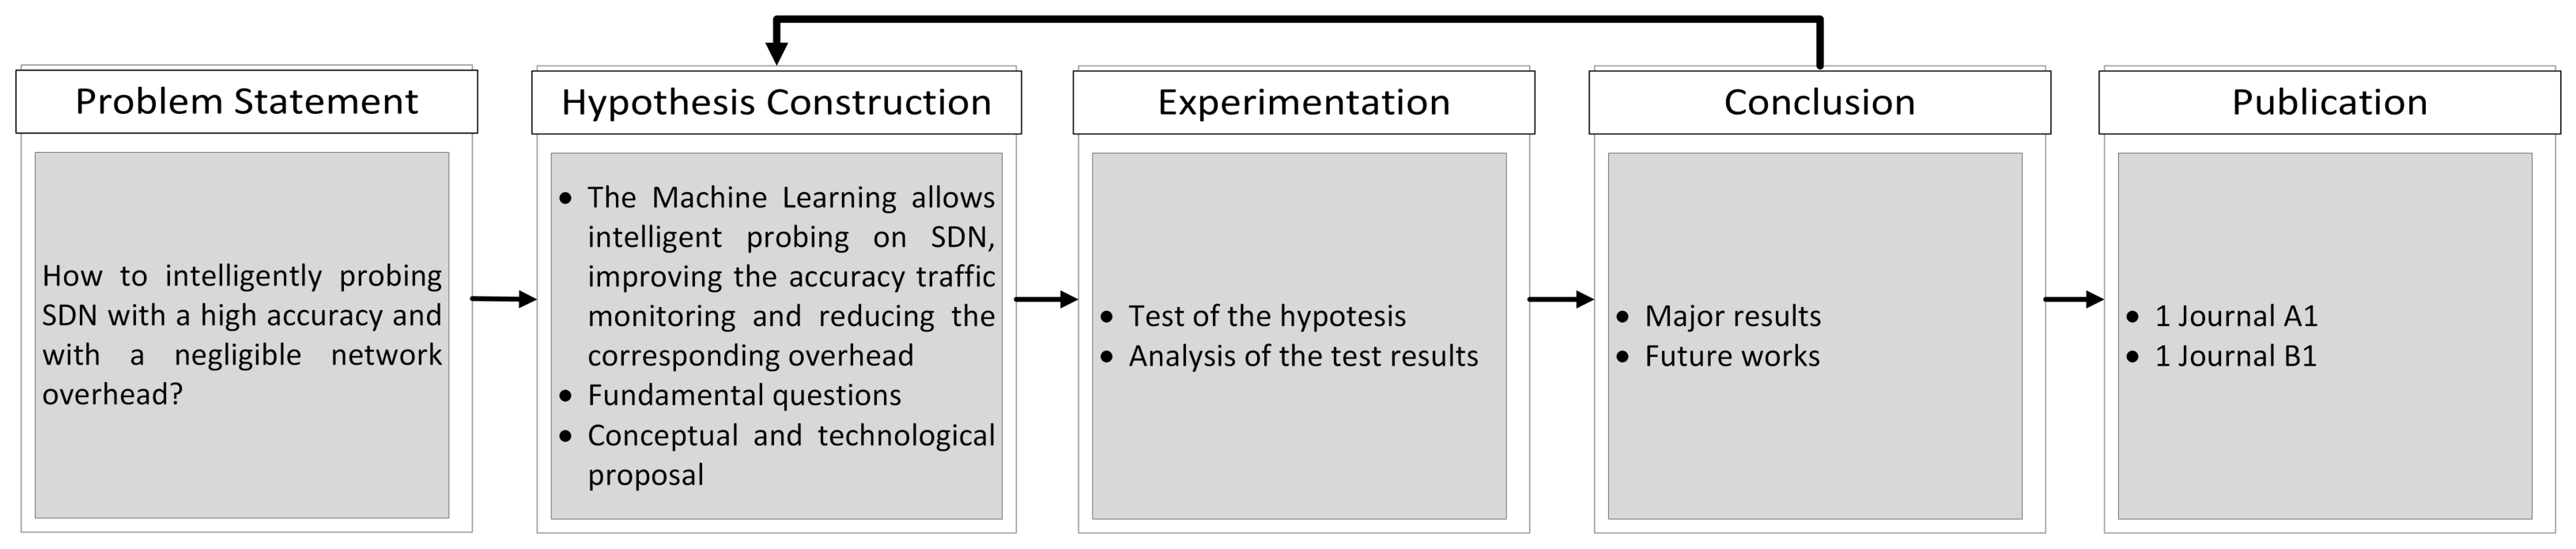
\includegraphics[width=1.0\columnwidth]{figures/scientific_research_process}
    \caption{Thesis phases}
    \label{fig:scientific_research_process}
\end{figure}

The organization of this document reflects the phases outlined above.
\begin{itemize}
    \item \textbf{This introductory chapter} presents the problem definition, raises the hypothesis, summarizes the contributions, and describes the overall structure of this master dissertation.
    
    \item \textbf{Chapter 2} reviews research about SDN, TE, Network Monitoring, ML, and KDN.
    
    \item \textbf{Chapter 3} presents the related works about SDN monitoring.
    
    \item \textbf{Chapter 4} presents a motivating scenario for the proposed approach. Also, this chapter introduces IPro, its architectural elements, and algorithmic representation.
    %introduces in detail the major contributions accomplished with this master dissertation.
    
    \item \textbf{Chapter 5} describes the experiments conducted to test the hypothesis, discusses the corresponding results, and presents implementation highlights.
    
    \item \textbf{Chapter 6} presents conclusions about the hypothesis and the fundamental questions, as well as opportunities for future works. 
    
    \item \textbf{Appendix} includes the list of papers in which the major results obtained during the development of this master dissertation have been published or submitted.
    
\end{itemize}
\chapter{Background}
\label{sec:background} 
%In this section, we introduce KDN, RL, and Q-learning briefly. We also present the related work about SDN monitoring.
The goal of this chapter is to present the background of the leading research topics touched in this master dissertation. In this way, this chapter starts showing the SDN concept and its architecture. After, this chapter reviews the TE concept and its use in SDN domains, including the basics of network monitoring. This chapter finishes discussing the ML concept. %This chapter finishes discussing some research works aimed to facilitate network monitoring.

\section{Software-Defined Networking}
\label{sec:background-sdn}

\begin{figure}[!ht]
    \centering
    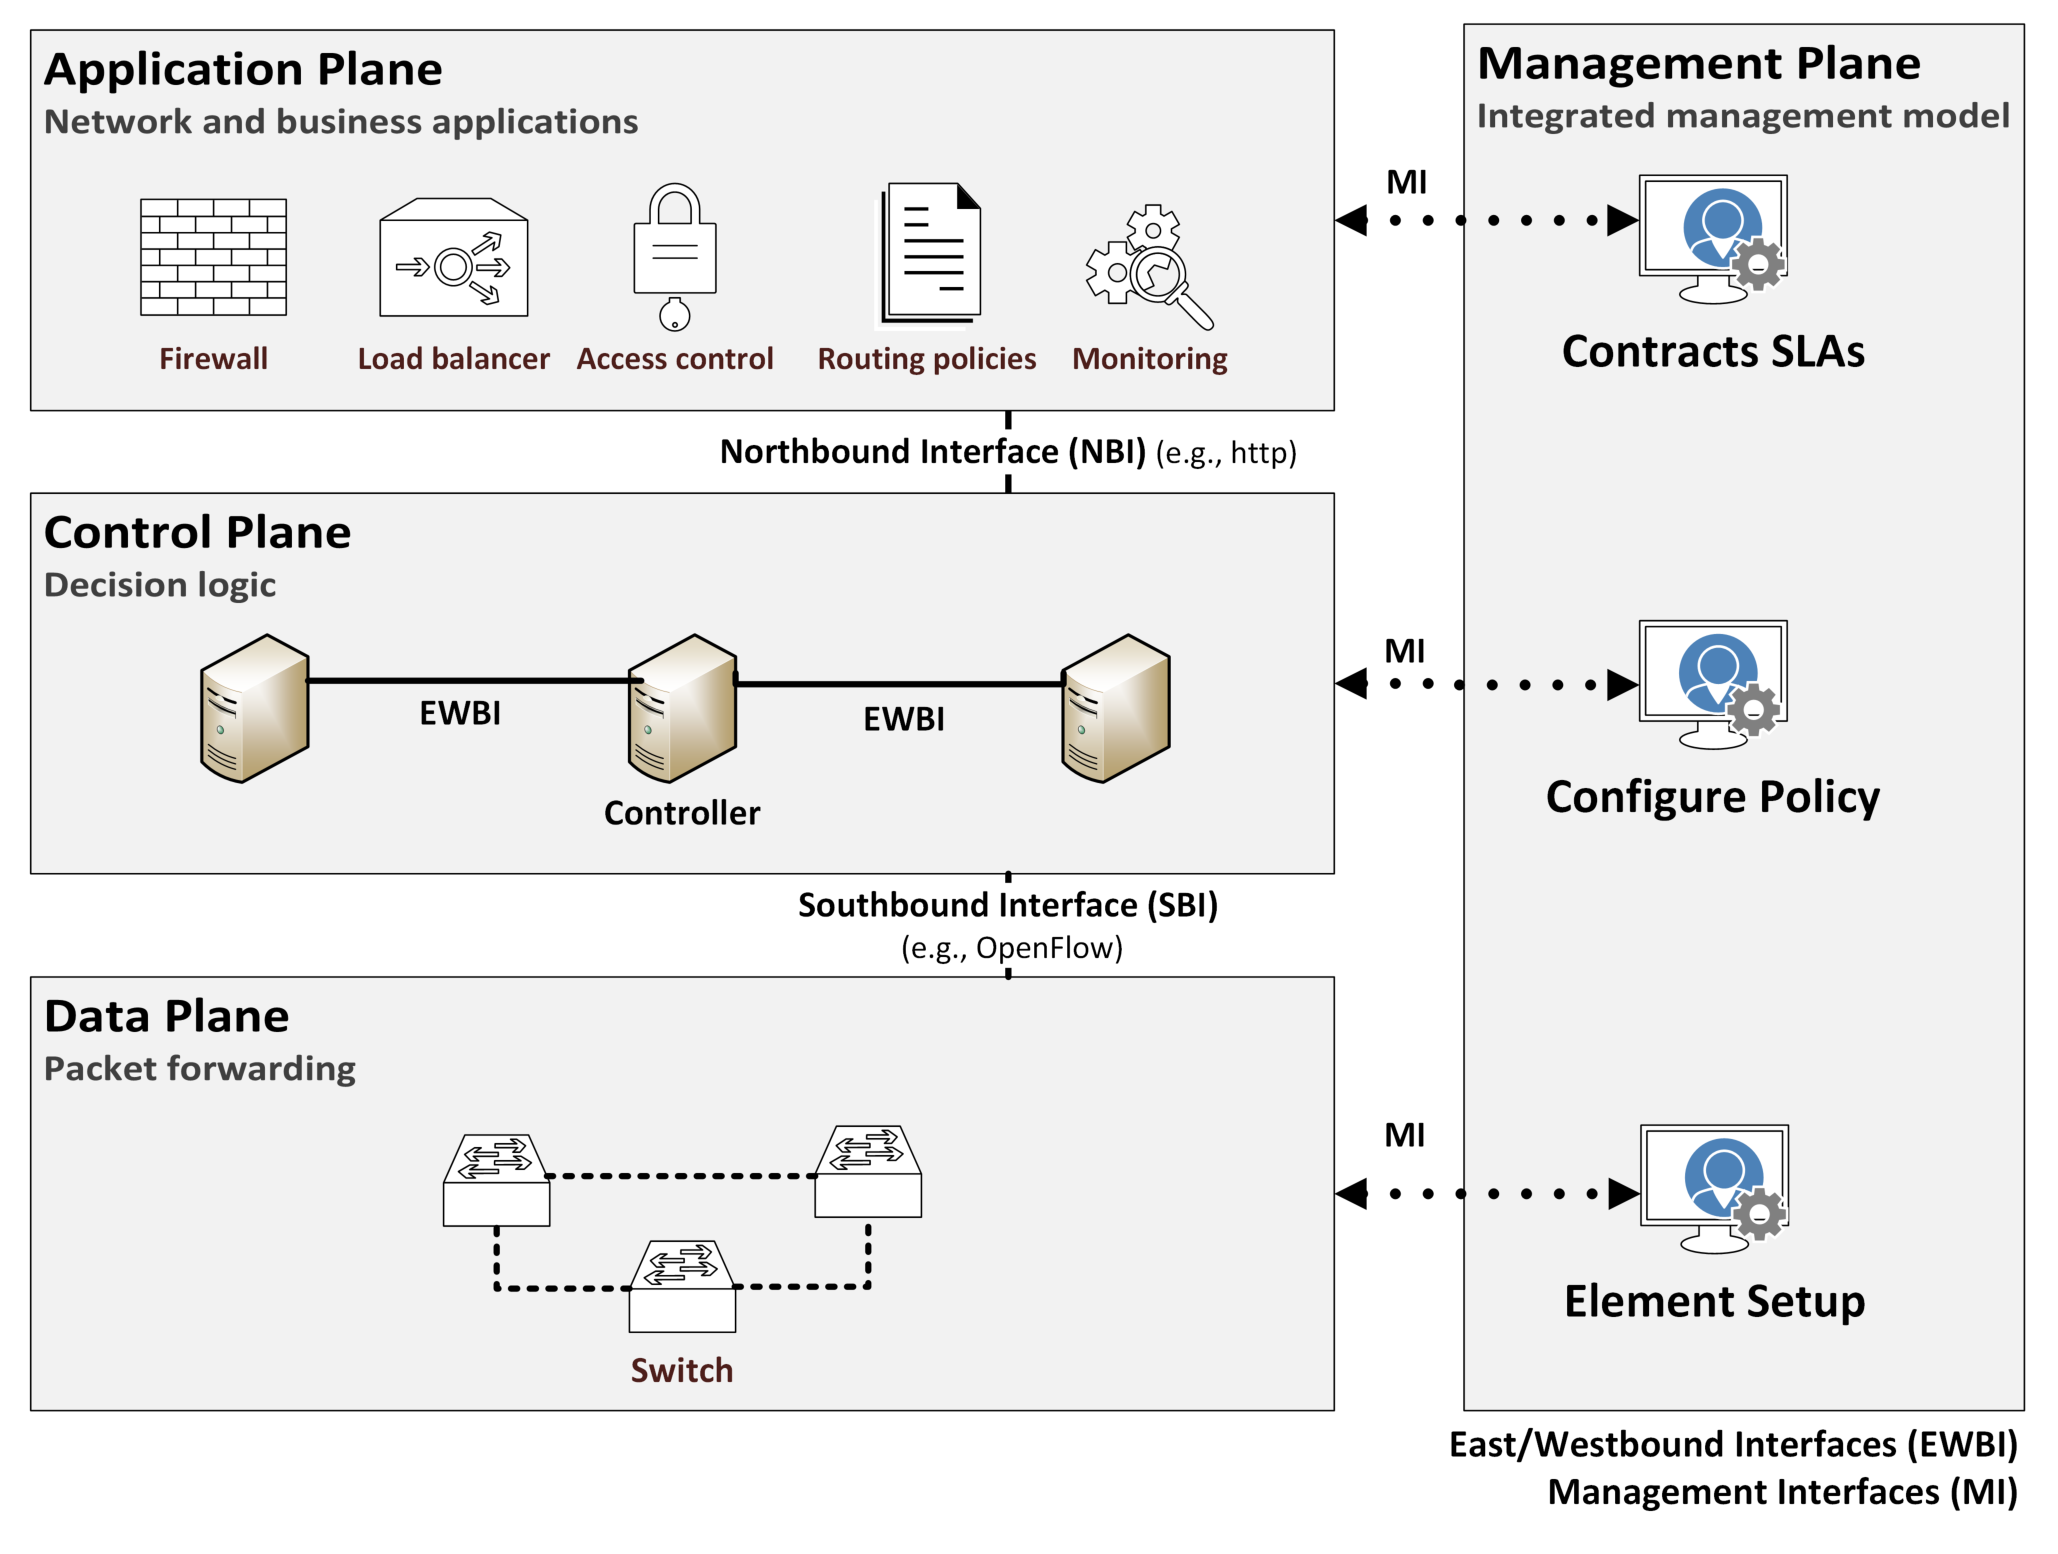
\includegraphics[scale=0.45]{figures/Figure_0_SDN_architecture}
    \caption{High-level SDN architecture}
    \label{fig:sdn_architecture}
\end{figure}

SDN represents one of the most well-known and attractive trends in academic and industry for defining the architecture of future networks \cite{ESTRADASOLANO2017150, feamster_2014:road_sdn}. SDN has some distinguishing features that define how it is different from traditional networking architecture. These features include \cite{kreutz_2015:sdn_comprehensive_survey, nunes_2014:survey_past_present_future}: (\textit{i}) clear separation of the control and forward function, (\textit{ii}) centralization of the control function, (\textit{iii}) implementation of the control function in software, (\textit{iv}) open standards, and (\textit{v}) Flow-based. These features make the SDN architecture more flexible, scalable, efficient and adaptable to the changing needs of the business \cite{herrera_2016:nfv_survey}. Furthermore, they make SDN a propitious scenario for efficiently and intelligently implementing monitoring techniques, particularly for TE.\\

Overall, SDN introduces an architecture with four planes \cite{onf_2014:sdn_architecture_overview}: management, application, control, and data (\textit{cf}. Figure~\ref{fig:sdn_architecture}). All these planes communicate with each other through interfaces. In particular, the Management Plane (MP) uses a set of Management Interfaces (MI) to exchange information and to control the other planes. The Application Plane (AP) communicates its network requirements to the Control Plane (CP) by NorthBound Interfaces (NBI). The CP defines East/Westbound Interfaces (EWBI) that enable to deploy a distributed controller for coping with large-scale and wide-area networks. The Data Plane (DP) communicates with CP by SouthBound Interfaces (SBI). Ideally,  all these interfaces should be standardized to allow easy replacement of devices and technologies. In practice, the OpenFlow protocol is the current \textit{de-facto} standard for the SBI because of its widespread use by vendors and research. All other interfaces are undergoing discussion and development.

\begin{itemize}
    \item \textbf{Management Plane} contains one or more solutions responsible for managing and coordinating each plane individually (\textit{e.g.}, network monitoring, performance management, configuring/planning resources, and enforcing both policies and contracts).
    
    \item \textbf{Application Plane} contains one or more applications that can serve different purposes (\textit{e.g.}, firewall, load balancer, access control, routing policies, and monitoring). Each application has access to a set of resources of one or more controllers through NBIs.
    
    \item \textbf{Control Plane} translates the requirements from AP at a specific network policy and enforces it over network elements through SBI. This plane contains one or more controllers (\textit{e.g.}, Floodlight, NOX, POX, and Ryu) that handle and coordinate the network devices.
    
    \item \textbf{Data Plane} contains a set of programmable network devices responsible for storing, forwarding and processing data packets. This plane depends on CP and MP to populate the forwarding tables and update their configuration.
\end{itemize}

%In \cite{onf_2013:sdn_architecture_overview}, the Open Networking Foundation (ONF) presents a high-level view of the SDN architecture along with its major components (Figure~\ref{fig:sdn_architecture}). At the bottom, the Data Plane (DP) is composed of network elements specialized in treating packages (forwarding), and it communicates with Control Plane (CP) by SouthBound Interfaces (SBI). The OpenFlow protocol \cite{mckeown_2008:openflow, kreutz_2015:sdn_comprehensive_survey, onf_2013:sdn_architecture_overview} is the most well-known open standard SBI because its widespread use by vendors and research. At the top, the Applications Plane (AP) implements and orchestrates the business logic and high-level networking functions (\textit{e.g.}, monitoring, routing policies, and access control). AP communicates its network requirements to the CP by NorthBound Interfaces (NBI). In the middle, CP translates application requirements and enforces them over network elements through SBI. CP also defines East/Westbound Interfaces (EWBI) that enable to deploy a distributed controller for coping with large-scale and wide-area networks. Furthermore, recent investigations have considered a Management Plane orthogonal to the whole SDN architecture for conducting integrated network management \cite{ESTRADASOLANO2017150}.

\section{Traffic Engineering}
\label{sec:background-te}

TE is emerging as an essential tool for selecting the optimal paths that different flows should follow to optimize resource utilization and satisfy the QoS requirements of each flow \cite{ian_2014:a_road_map_sdn, shu_2016:traffic_measurement_management}. According to the Internet Engineering Task Force (IETF), TE aims to evaluate and optimize network performance, QoS, and user experience of operational IP networks \cite{feamster_2014:road_sdn, awduche_2002:overview_ti, wang_2008:overview_routing_ti}. TE, in SDN, focuses on \cite{ian_2014:a_road_map_sdn}:

\begin{itemize}
    \item 
    \textbf{Flow Management (FM)} controls network resources appropriately when traffic congestion occurs in network nodes. FM maps and controls the traffic flow to steer traffic most efficiently. For example, when a switch receives flows that do not match any rule in the flows table; it forwards these flows to the controller. The controller analyzes this flow and decides to install it a new forwarding rule in the switches or to remove it. If the traffic consists of a high number of new flows or not match flows, it can generate a significant network overhead and latency at both CP and DP. FM looks for avoiding network overhead and providing a trade-off between load-balancing and latency.
    \item 
    \textbf{Fault Tolerance (FT)} seeks to ensure the immediate, transparent and graceful recovery of the network when a failure occurs in any of its nodes. FT provides mechanisms that enhance network integrity and adopts policies emphasising network survivable. For example, to increase the networking resiliency of SDN, FT could introduce a mechanism for link or node failures. This mechanism could specify alternative ports and paths that enable the switch to change the forwarding path in the policy-based routing without requiring a round trip to the controller.
    \item 
    \textbf{Topology Update (TU)} manages the capacity of the network to carry out planned changes (\textit{i.e.}, it aims to update the policies of the network in real time and ensure their application in each flow). For example, since the centralized controllers manage all switches, these can dynamically configure the global network policy rules. TU should guarantee consistency of the network policies across the switches so that each packet or flow should be handled by either the old policy or the new policy, but not by the two.
    \item 
    \textbf{Traffic Analysis/Characterization (TAC)} deals with the monitoring and verification of compliance with network performance goals to evaluate and debug the effectiveness of the applied TE methods. TAC focuses on mechanisms for monitoring the network, debugging errors, fault detection, data collection, and so on. In particular, TAC is the essential prerequisite for traffic analysis, and it is closely related to discovery the network failures and the prediction of link congestion.
\end{itemize}

An essential requirement for achieving TE is to provide accurate and reliable network monitoring (\textit{e.g.}, to perform TE \cite{al_2010:hedera}, it is necessary to correctly detect large flow aggregates in minutes and pick better routes for these flows). Many network management tasks such as traffic accounting, load balancing, and performance diagnosis all rely on accurate and timely monitoring of a large variety of traffic at different time-scales \cite{machado_2014:towards_SLA_Policy,tangari_2017:decentralized_monitoring,al_2010:hedera,benson_2011:microte}. 

\section{Network Monitoring}
\label{sec:background-ntm}

\subsection{Monitoring Operations}
\label{subsec:monitoring-operations}

Network Monitoring collects measurements of Key Performance Indicators (KPI) and events (\textit{e.g.}, bandwidth utilization and link status) to process them into more meaningful metrics, called Aggregate Metrics (\textit{e.g.}, average delay and network availability) \cite{mohan2011:active_passive}. Generally, network monitoring can be roughly classified into five phases: \textit{Collection, Preprocessing, Transmission, Analysis}, and \textit{Presentation} of the data \cite{tsai_2018:network_monitoring_review}. Figure~\ref{fig:monitoring_phases}, depicts the classification of operation phases in network monitoring.

\begin{figure}[!ht]
    \centering
    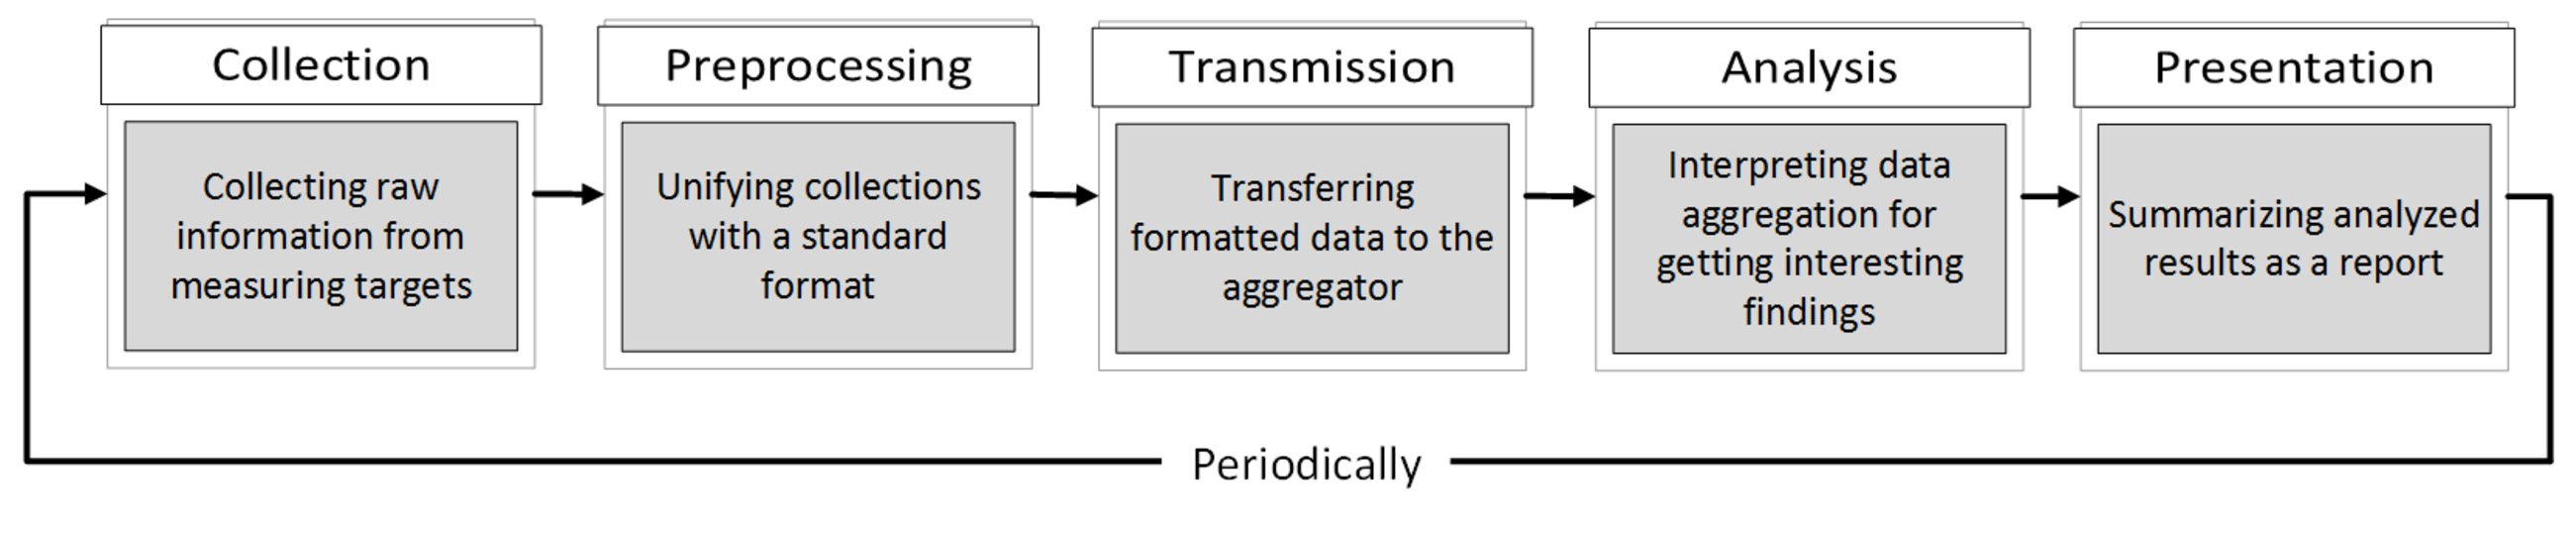
\includegraphics[scale=0.37]{figures/NetworMonitoringPhases}
    \caption{Classification of network monitoring operations (adapted from \cite{tsai_2018:network_monitoring_review})}
    \label{fig:monitoring_phases}
\end{figure}

\begin{itemize}
    \item \textit{Collection:} This phase raises three primary considerations namely, means, target, and probing interval. The means refers to how the data are to be collected. The target relates to the devices to be observed, and the probing interval indicates how often the data should be collected from switches.
    \item \textit{Preprocessing:} This phase is responsible for aggregating and turning the collected data into some statistical format. Furthermore, it helps to itemize and track the measurement results.
    \item \textit{Transmission:} This phase is responsible for carrying itemized data to the analytic station. The Simple Network Management Protocol (SNMP) and the Network Configuration Protocol (NETCONF) are typical protocols used to exchange messages in the transmission phase. These protocols provide a data delivery interaction between agents and the station.
    \item \textit{Analysis:} This phase generates statistics and identifies particular events. Some methods perform traffic analysis based on payload or host behavior, whereas other methods examine communication patterns \cite{Bujlow_2012:traffic_classificatiom_c5, dong_2012:traffic_clasification_ml}. The analysis results provide network status information to TE and fault management applications. 
    \item \textit{Presentation:} This phase exports the analysis results in tables, graphs, and reports. For example, Isolani \textit{et al.} \cite{isolani_2015:interactive} proposed an SDN Interactive Manager that provides data visualization via traffic graphs.
\end{itemize}{}

A critical task in network monitoring is to achieve a better performance in terms of low overhead (\textit{e.g.}, CCO and CUC) and high MA when measuring the network status. To achieve better performance, it is essential an accurate and timely collection of flow statistics \cite{rendon2014:monitoring}.

\subsection{Network Monitoring Techniques}
\label{subsec:monitoring-approaches}

In SDN, network monitoring techniques can be classified into two categories \cite{mohan2011:active_passive,Ningning_2003:probing_techniques}: push-based (called passive monitoring) and pull-based (called active monitoring). Although the focus of this dissertation is on the pull-based technique, both push-based and pull-based will be discussed briefly.

\begin{figure}[!ht]
        \centering
        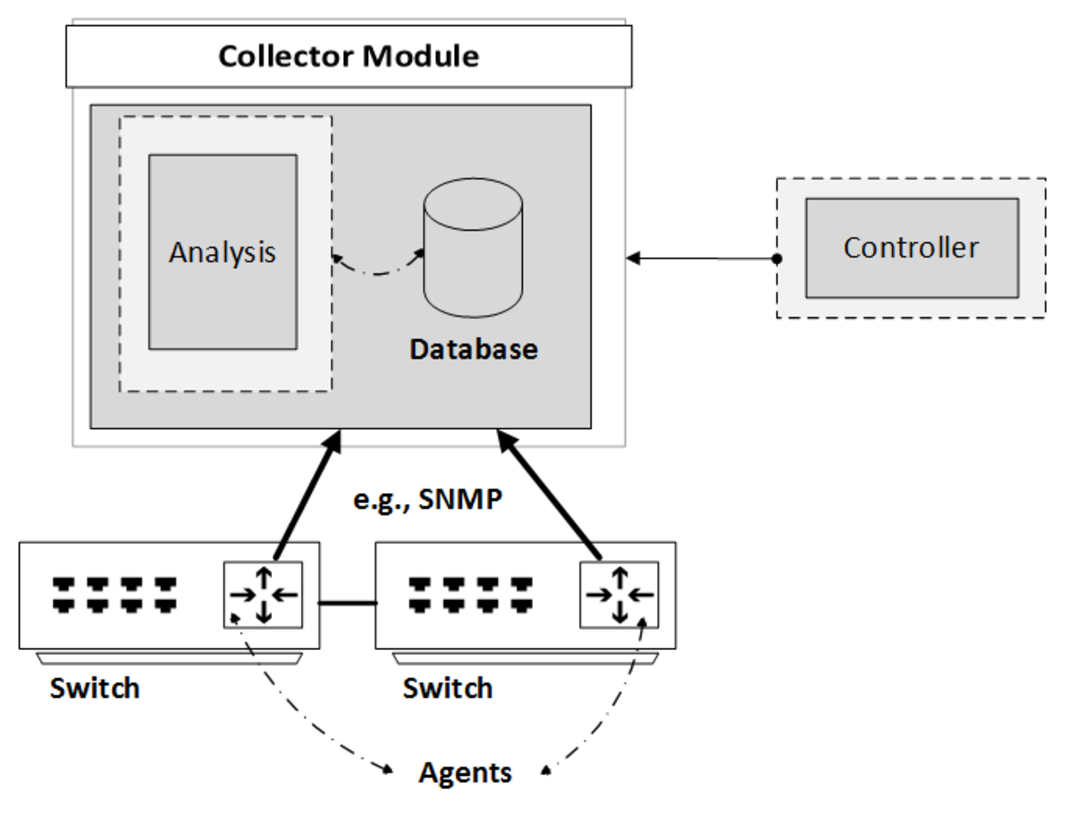
\includegraphics[scale=0.49]{figures/Push-Based}
        \caption{Push-based monitoring}
        \label{fig:push-based}
\end{figure}

\begin{itemize}
    \item In the \textbf{Push-based} approach \cite{claise2004:cisco_netflow,phaal2001:inmon_sflow}, the controller observes the statistics information supplied by a collector module without influencing in the performance of the network (\textit{cf.} Figure~\ref{fig:push-based}). In this approach, the statistical information is collected by agents placed inside switches (\textit{e.g.}, NetFlow \cite{claise_2004:cisco}, jFlow \cite{myers_1999:jflow}, sFlow \cite{wang_2004:sflow}), which observe and send the network traffic to the collector module using a monitoring protocol (\textit{e.g.}, SNMP and NETCONF). The collector module is responsible for analyzing and storing this network traffic to make it available to the controller.
    
    Although Push-based approach does not intervene in the performance of the network, several factors hinder its applicability. First, additional elements are necessary in the hardware and software of switches. Second, when the traffic varies dynamically, switches frequently detect no-matching packets in the flow table and, as a result, massive statistical reports are sent to the controller. These massive reports can cause significant CCO \cite{aslan_2016:impact} and CUC \cite{su_2014:flowcover}. Third, the push-based approach requires full access to network devices, which could raise privacy and security issues.
    
    %\item \textbf{Pull-based} injects test packages (\textit{e.g.}, ping and traceroutes) into the network for measuring the response and checking the result for important metrics such as latency, jitter, throughput, and packet loss. 
    \item In the \textbf{Pull-based} approach, the controller probes one, a set, or all switches using Read-State messages to retrieve statistics from switches (\textit{cf.} Figure~\ref{fig:pull-based}). There are two variations of Read-State messages: \textit{Request} and \textit{Reply}. The  \textit{Request} messages are sent from the controller to switches to request the specific statistical information. The \textit{Reply} messages, on the other hand, are sent from the switches to the controller, delivering the required statistical information.
    
    \begin{figure}[!ht]
        \centering
        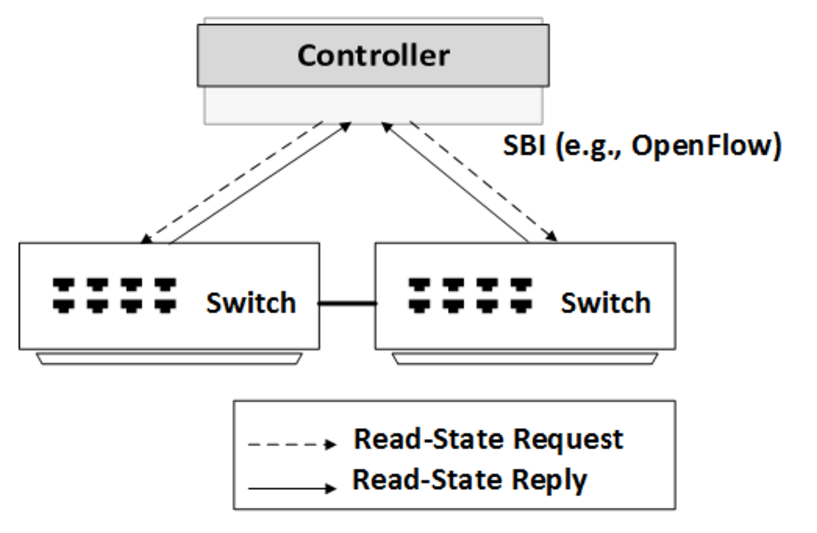
\includegraphics[scale=0.6]{figures/Pull-Based}
        \caption{Pull-based monitoring}
        \label{fig:pull-based}
    \end{figure}
       
    This approach provides flexibility, since it can asynchronously communicate with switches to request the specific state information and control the size of statistical reports. Nonetheless, CCO can also be introduced in the pull-based approach because of the probing interval. This overhead can lead to overload the controller (\textit{i.e.}, increase CUC) and significantly interfere with essential SDN functions, such as packet forwarding and route updating \cite{Malboubi_2015:SNIPER}.
\end{itemize}

This master dissertation focuses on the pull-based approach because:
\begin{itemize}
    \item It allows requesting specific statistical information from one, a set, or all switches asynchronously, allowing the controller to collect statistical information flexibly and control the size of statistical reports.
    \item It does not require changes in the software and hardware of switches because the controller only needs Read-State messages, intrinsic in SDN switches, to retrieve statistical information.
\end{itemize}

\section{Machine Learning}
\label{sec:background-ml}

The quantity of data that flows through communication networks is increasing exponentially. The extraction of knowledge from this data is becoming increasingly important to perform efficient monitoring and management of the network. ML is a tool used to extract useful knowledge from the data and make appropriate decisions \cite{sara_2018:ml_cognitive_network_management,Mowei_2017:ml_Workflow,stampa_2017:DL_optimization}.\\

ML includes a set of techniques that can automatically detect patterns in the data (patterns that do not conform to the normal network behavior) to identify previously unseen events and thus to detect network anomalies and to predict future data \cite{murphy_2012:ml_probabilistic,bishop_2006:pattern_recognition}. The possibilities that emerge from the use of ML in networking context are various \cite{Boutaba2018}, some examples are:

\begin{itemize}
    \item \textit{Network traffic prediction:}  Li \textit{et al.} \cite{li2016predicting} proposed an ML technique that focus is on predicting incoming and outgoing traffic volume on an inter-data center link dominated by elephant flows. Poupart \textit{et al.} \cite{Poupart_2016:online} explored the use of ML for flow size prediction and elephant flow detection. Chen \textit{et al.} \cite{chen2016predicting} investigated the possibility of reducing the cost of monitoring and collecting traffic volume, by inferring future traffic volume based on flow count only.  %\cite{sun_2016:cs2p}.,chen_2016_predicting_traffic}.
    
    \item \textit{Resource management:} Bojovic \textit{et al.} \cite{bojovic2012cognitive} designed an ML-based radio admission control mechanism to guarantee QoS for various services, such as voice, data, video and FTP while maximizing radio resource utilization in long term evolution (LTE) networks. Vassis \textit{et al.} \cite{vassis2014admission} proposed an adaptive and distributed admission control mechanism for variable bitrate video sessions, over ad hoc networks with heterogeneous video and HTTP traffic. Quer \textit{et al.} \cite{quer2011cognitive} developed an admission control mechanism for VoIP calls in a WLAN. They employed ML to predict the voice call quality as a function of link-layer conditions in the network.
    
    \item \textit{Fault management:} Snow \textit{et al.} \cite{snow2005assessing} used ML to estimate the dependability of a 2G wireless network, which is used to characterize availability, reliability, maintainability, and survivability of the network. Lu \textit{et al.} \cite{lu2009using} use a manifold learning technique to automatically extract failure features and generate failure prediction. Pellegrini \textit{et al.} \cite{pellegrini2015machine} proposed an ML-based framework to predict the remaining time to failure of applications.
    
    \item \textit{Congestion control:} Liu \textit{et al.} \cite{liu2003end} proposed an approach using ML for inferring the cause of packet loss in hybrid wired-wireless networks. Fonseca and Crovella \cite{fonseca2005bayesian} focused on detecting the presence of packet loss by differentiating Duplicated ACKs caused by congestion losses and reordering events. Jayaraj \textit{et al.} \cite{jayaraj2008loss} tackled the classification of congestion losses and contention losses in optical burst switching networks.% \cite{dong_2015:pcc}.
\end{itemize}{}

Furthermore, ML has been used successfully in other domains, including agriculture \cite{efcastillo_2016:agriculture, efcastillo_2015:agriculture, ZHANG_2005:agriculture}, economics \cite{kim_2004:usefulness, nielsen_2004:local}, and cybersecurity \cite{Dua_2011:DM_ML_Cybersecurity, Thuraisingham_2003:ciber}.\\

ML can be divided into three categories, based on how the learning is achieved \cite{ayodele_2010:introduction, bishop_2006:pattern_recognition}:

\begin{itemize}
    \item \textbf{Supervised Learning (SL)} requires a set of instances, commonly known as training data, which are used to define the behavior of algorithm. The training data consists of a set of attributes and an objective variable (also called class), which is intended to be classified or predicted. When the domain of the attribute is categorical\footnote{A domain is defined as categorical if it is finite (discrete numerical values) and unordered}, the problem is known as classification or pattern recognition, and when the domain of the attribute is numeric\footnote{A numeric domain consists of real numbers} value, the problem is known as regression. The most representative algorithms of SL are: Bayesian Networks, Support Vector Machines, k-Nearest Neighbors, Decision Trees, and Neural Networks \cite{Mowei_2017:ml_Workflow,Boutaba2018}.
    
    \item \textbf{Unsupervised Learning (UL)} explores the structure of a non-tagged dataset (without target variable). This method reveals unexpected characteristics (patterns) and generates new groups (each with different identifiable properties). The unsupervised learning algorithms are divided into three relevant categories: 
    
    \begin{itemize}
        \item \textit{Hierarchical Algorithm} aims to obtain a hierarchy of clusters, called dendrogram, that shows how the clusters are related to each other \cite{Grira_2004:ml_techniques}.
        
        \item \textit{Density Algorithm} finds the areas with the highest data density, leaving aside the sparsely populated regions, which are considered border points or noise \cite{rehman_2006:density_based_clustering}.
        
        \item \textit{Clustering Partitional Algorithms} aims to directly obtain a single partition of the collection of items into clusters \cite{Grira_2004:ml_techniques}.
    \end{itemize}{}
    
    \item \textbf{Reinforcement Learning (RL)} is an iterative process in which an agent learns a decision-making process by interacting with the environment (\textit{cf.} Figure~\ref{fig:rl}). The agent is aware of the state of the environment and takes actions that produce changes of state. For each action, the agent receives a reward depending on how good was the action taken. The goal of the agent is to maximize the total reward it receives over time.
    
    \begin{figure}[!ht]
        \centering
        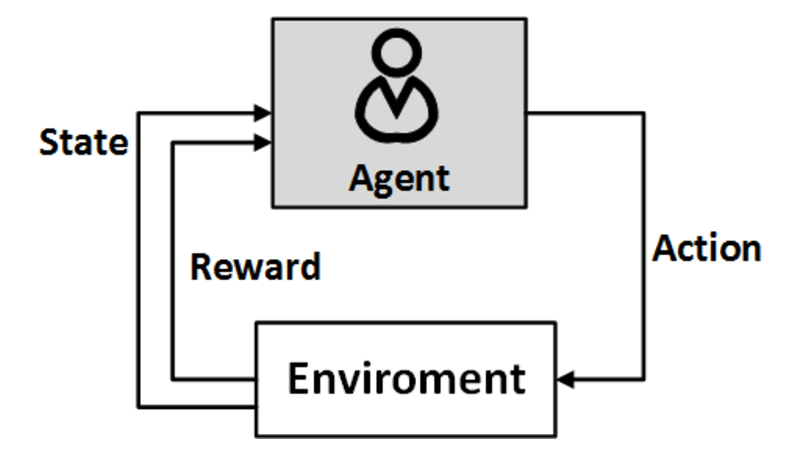
\includegraphics[scale=0.6]{figures/rl}
        \caption{RL Process}
        \label{fig:rl}
    \end{figure}
    
    RL is best suited for making cognitive choices, such as decision making, planning, and scheduling. For instance, RL has been successfully applied to complex problems such as board games \cite{tesauro_1995:temporal}, job-shop scheduling \cite{yoshimoto_1999:application}, elevator dispatching \cite{crites_1998:elevator}, and motor control tasks \cite{doya_2000:reinforcement}, either simulated or real \cite{schaal_1994:robot}.
    
\end{itemize}
\section{Final Remarks}
\label{sec:final_remarks_kap2}

Initially, in this chapter, the concept of the SDN  and the architectural features that make the SDN more flexible, scalable, efficient, and adaptable to the changing needs of the business were detailed. Subsequently, the fundamental concepts about TE and network monitoring in the SDN context were described, along with the monitoring techniques related to traffic collection. Finally, the ML concept was introduced, along with its categories and its use in the networking context. This master dissertation considers these concepts for proposing an approach (\textit{cf.} Chapter~\ref{chapter:intelligent_probing}) that focuses on optimizing the probing interval regarding CCO and CUC.

%\afterpage{\null\newpage}
\newpage{\null\newpage}
\newpage
\chapter{State-of-Art}
\label{sec:state-of-art}

This chapter provides an overview of the paramount efforts around SDN traffic monitoring. In this way, this chapter starts presenting the traffic monitoring proposals for SDN with a higher impact on the research community. This chapter finishes discussing these research works.

\section{SDN Monitoring}
\label{sec:related_work}

In general, network monitoring is a fundamental topic and an essential requirement for achieving TE \cite{feamster_2014:road_sdn,Boutaba2018,8255757}. IP networks are usually monitored with mechanisms such as NetFlow \cite{claise_2004:cisco}, jFlow \cite{myers_1999:jflow}, and sFlow \cite{wang_2004:sflow}. These mechanisms use probes connected to special modules placed inside switches. These probes collect either complete or sampled traffic statistics and send them to a central collector. NetFlow and JFlow are both proprietary solutions and incur a considerable up-front licensing and setup cost to be deployed in a network. sFlow is less expensive to deploy, but it is not widely adopted by the vendors \cite{chowdhury_2014:payless}. It is important to highlight that the network monitoring in traditional IP networks can lead to high overhead and significant switch resource consumption \cite{Curtis_2011:Mahout}. Recent research efforts have harnessed the power of SDN to propose solutions for such monitoring. This section presents some approaches to network monitoring found in the literature.\\

Raumer \textit{et al.} introduced an application for the Quality of Service (QoS) monitoring, called MonSamp \cite{raumer_2014:monsamp}. MonSamp completely moves monitoring capabilities out of the controller and provides fully processed information to the applications by a Northbound API. To traffic collect, MonSamp provides sampling algorithms that can adapt to both current network load and the QoS requirements. In particular, MonSamp suggests decreasing the sampling rate under high traffic load. MonSamp uses thresholds to adjust the amount of monitoring overhead that is forwarded by the switches to allow a certain MA.\\

Van Adrichem \textit{et al.} proposed OpenNetMon \cite{van_2014:OpenNetMon} to monitor network throughput, packet loss rates, and network delays continuously. OpenNetMon uses an adaptive probing mechanism to extract statistical information from the switches. The adaptive probing mechanism increases the rate of the queries when the flow rates differ between samples (increases the MA, CCO, and CUC) and decreases when flows stabilize (reduces the MA, CCO, and CUC).\\
%Van Adrichem \textit{et al.} proposed OpenNetMon \cite{van_2014:OpenNetMon} to monitor network throughput, packet loss rates, and network delays continuously. First, to measure the throughput rate, it only probes the last switch on the forwarding path using an adaptive frequency. This switch returns the number of packets (S) of each flow in the sampling interval (T), and the forwarding path throughput is obtained as S/T. Second, to calculate packet loss rates, it probes the first and last switches on the forwarding path to obtain counter statistics. The packet loss rate of this forwarding path is obtained as the difference between the increment of the first and last counter in a measurement cycle divided by the time. Third, to calculate the delay, the OpenNetMon sends probe messages to data layers of the forwarding path, these messages get through all nodes of the path and finally return to the controller, where the delay is obtained by calculating time differences.\\

Tahaei \textit{et al.} proposed a multi-objective network measurement mechanism \cite{tahaei_2017:multi-objective} to overcome the CCO, CUC, and MA in a real-time environment. To strike the trade-off between the MA and CCO, this mechanism uses an elastic probing for the collection of statistics from the switches. The elastic probing adaptively adjusts probing frequency based on the behavior of link utilization. In particular, it increases the probing frequency according to the bandwidth fluctuation of the flows (\textit{i.e.}, to higher bandwidth fluctuation higher probing frequency). Tahaei \textit{et al.} also made an extension to his previous work. This extension proposed a generic architecture for flow measurement in a data-center network, which applies in both single and multiple-controller \cite{tahaei_2018:cost_effective}. The three main features of this architecture are: first, it utilizes local controllers to pull flow statistic and forwards statistics to an upper layer application. Second, it has a coordinator level on top of all the local controllers connecting to the switches. Third, it is implemented as a standard northbound interface, which can utilize both fixed and adaptive polling systems.\\

Tootoonchian \textit{et al.} proposed OpenTM \cite{Tootoonchian_2010:opentm} to estimate the traffic matrix using OpenFlow statistics (\textit{e.g.}, bytes and packet counters). OpenTM proposes several heuristics (\textit{e.g.}, last switch, round robin, uniform random selection, and non-uniform random selection) to (i) choose an optimal set of switches to be monitored for each flow and (ii) keep the trade-off between MA and CCO. After a switch has been selected, OpenTM probes the switch selected continuously for collecting flow level statistics. The choice of a heuristic defines the level of MA and CCO. For instance, the use of the last switch heuristic results in the most accurate traffic matrix but imposes a substantial overhead on edge switches. The price to use the uniform random selection heuristic is to lose some accuracy.\\

Chowdhury \textit{et al.} proposed a flow measurement framework called PayLess \cite{chowdhury_2014:payless}. It is designed as a component of the OpenFlow controller, and it provides a RESTful API for flow statistics collection at different aggregation levels (\textit{e.g.}, flow, packet, and port). In particular,  this framework is responsible for parsing request commands from the application level of tasks and transforming these commands into path planning on some switches. PayLess adjusts the probing frequency to balance the CCO and MA. To achieve this balance, Payless relies on OpenTM \cite{Tootoonchian_2010:opentm} to select only important switches to be monitored. Nonetheless, instead of continuously probing a switch, PayLess offers an adaptive scheduling algorithm for probing that achieves the same level of accuracy as continuous probing with much less overhead.\\

Peng \textit{et al.} proposed a traffic management solution (HONE) based on joint statistical information from the OpenFlow network and end hosts \cite{Sun_2015:HONE}. HONE uses software agents placed inside end hosts and a module that interacts with OpenFlow switches. HONE integrates information from the OpenFlow network and end hosts to present a diverse collection of fine-grained monitoring statistics. Furthermore, HONE offers two techniques to process flow statistics: The first technique, known as the lazy materialization of the measurement data, it uses database-like tables to represent the statistical information collected from hosts and network devices. Lazy materialization allows that both the controller and host agents use the statistical information collected in multiple management tasks. The second technique offers data parallel streaming operators for programming the data-analysis logic. The operators can also be used in a hierarchical fashion for aggregate analysis among multiple hosts.\\

Phan \textit{et al.} proposed a scalable framework called SDN-Mon \cite{phan2017:sdn_mon}. SDN-Mon decouples monitoring from existing forwarding tables to allow more fine-grained and flexible monitoring. This framework uses a controller-side module and a switch-side module. The controller-side module defines a set of monitoring match fields based on the requirements of applications to allow higher flexibility. The switch-side module process the monitoring functionality of the framework to reduce the CCO. Phan \textit{et al.} \cite{phan2017:adaptive_sdn_mon} also proposed a mechanism that supports distributed monitoring capability of SDN-Mon. This extension introduces three additional modules: the switch module, the controller module, and the external module, which allow SDN-Mon can automatically assign the monitoring load to multiple monitoring switches in a balanced way and eliminate duplicated monitoring entries.\\

Liao \textit{et al.} proposed a solution for latency monitoring called LLDP-looping \cite{liao_2018:LLDP-looping}. LLDP-looping monitors the latency of all network links by using agents placed inside switches and a controller module that interacts with them. The controller module uses a greedy algorithm to inject probe packets (i.e., time-stamped Link Layer Discovery Protocol (LLDP) packets) to a selected set of switches to minimize the CCO. The agents, first, forces to each probe packet to loop around a link for three times, then, calculates the RTT of the LLDP packet.\\

Jose \textit{et al.} \cite{jose_2011:online_measurement} presented a monitoring framework that use secondary controllers to identify and monitor aggregates flows using a small set of rules that changes dynamically with traffic load.  In this framework, on the one hand, the switches match packets against a small collection of wildcard rules available in Ternary Content Addressable Memory (TCAM), then the counter of the matched highest priority rule is updated.  On the other hand, the controllers only read and analyze the relevant counters from the TCAM with fixed time intervals. Furthermore, the authors proposed a heavy hitters algorithm that identifies large traffic aggregates, striking a trade-off between MA and switch overhead.\\

Tangari \textit{et al.} proposed a decentralized approach for resources monitoring \cite{tangari_2017:decentralized_monitoring}. This approach achieves high reconfiguration reactivity with acceptable accuracy and negligible CCO. It uses local managers, distributed over the network, to adaptively reconfigure the network resources (under their scope of responsibility). Furthermore, it uses entities installed on local managers to support a wide range of measurement tasks and requirements regarding monitoring rates and information granularity levels. Tangari \textit{et al.} also extended the previous work by proposing a self-adaptive and decentralized framework for resource monitoring  \cite{Tangari_2018:adaptive_decentralized_monitoring}. This framework uses a self-tuning, adaptive monitoring mechanism that automatically adjusts its settings based on the traffic dynamics, which improves the MA.

\section{Research Gaps}

\fontsize{9}{8}\selectfont
\begin{table*}[!htp]
\begin{center}
\scriptsize
\begin{longtable}{P{0.8cm}|P{0.2cm}|P{0.2cm}|P{0.2cm}|P{0.2cm}|P{11.8cm}}
\caption{Traffic Monitoring in SDN -- H $\rightarrow$ High and L $\rightarrow$ Low} \\
\hline
\multicolumn{1}{c|}{\textbf{Work}} & \multicolumn{1}{c|}{\textbf{\rotatebox[origin=c]{90}{Accuracy}}} & \multicolumn{1}{c|}{\textbf{\rotatebox[origin=c]{90}{Overhead}}} & \multicolumn{1}{c|}{\textbf{\rotatebox[origin=c]{90}{Resources-Cost}}} & \multicolumn{1}{c|}{\textbf{\rotatebox[origin=c]{90}{Flexibility-Scalability}}} & \multicolumn{1}{c}{\textbf{\rotatebox[origin=c]{0}{Description}}} \\ 
\hline 
\endfirsthead

\multicolumn{6}{c}%
{{\bfseries \tablename\ \thetable{} -- Continued from previous page}} \\
\hline 
\multicolumn{1}{c|}{\textbf{Work}} & \multicolumn{1}{c|}{\textbf{\rotatebox[origin=c]{90}{Accuracy}}} & \multicolumn{1}{c|}{\textbf{\rotatebox[origin=c]{90}{Overhead}}} & \multicolumn{1}{c|}{\textbf{\rotatebox[origin=c]{90}{Resources-Cost}}} & \multicolumn{1}{c|}{\textbf{\rotatebox[origin=c]{90}{Flexibility-Scalability}}} & \multicolumn{1}{c}{\textbf{\rotatebox[origin=c]{0}{Description}}} \\ 
\hline 
\endhead

\hline \multicolumn{6}{r}{{Continued on next page}} \\ \hline
\endfoot

\hline \hline
\endlastfoot

%###################################### First Stream ###################################################################
\RaggedRight \cite{su_2014:flowcover}& H & L & H & L & \justifying\noindent{\textcolor{reviewer3}{A heuristic algorithm (Greedy) is used to minimize the CCO, obtain the polling scheme efficiently, and handle flow changes}} & \hline

\RaggedRight \cite{chowdhury_2014:payless}& H & H & H & H & \justifying\noindent{Adaptive sampling algorithms are used to tune the load level generated by monitoring process} & \hline

\RaggedRight \cite{raumer_2014:monsamp}& H & H & H & H & \justifying\noindent{Thresholds are used to adjust the load level generated by monitoring process} & \hline

\RaggedRight \cite{van_2014:OpenNetMon}& H & H & H & L & \justifying\noindent{An adaptive fetching mechanism monitors per-flow metrics, such as throughput, delay, and packet loss} & \hline

\RaggedRight \cite{tahaei_2017:multi-objective}& H & H & L & H & \justifying\noindent{An adaptive flows statistical collection method is used to adjust the polling intervals} & \hline

\RaggedRight \cite{Tootoonchian_2010:opentm}& H & H & L & H & \justifying\noindent{Routing information from the controller and flow forwarding path information are used to monitor the link utilization} & \hline
%###################################### Second Stream ###################################################################
\RaggedRight \cite{Sun_2015:HONE}& H & L & H & L & \justifying\noindent{Software agents residing on hosts interact with network devices to perform monitoring tasks} & \hline

\RaggedRight \cite{jose_2011:online_measurement}& H & L & H & L & \justifying\noindent{A small set of matching rules and secondary controllers are used to identify and monitor aggregate flows} & \hline

\RaggedRight \cite{phan2017:sdn_mon}& H & L & H & L & \justifying\noindent{Monitoring is decoupled from existing forwarding tables and uses customized software agents in the switches to process their monitoring functionality} & \hline

\RaggedRight \cite{liao_2018:LLDP-looping}& H & L & H & L & \justifying\noindent{It injects time-stamped LLDP packets into switches to monitor the network latency} & \hline
%###################################### Third Stream ###################################################################
\RaggedRight \cite{tangari_2017:decentralized_monitoring}& H & L & H & L & \justifying\noindent{Local managers and entities are used to reconfigure the network resources and support monitoring tasks at different granularity level} & \hline

\RaggedRight \cite{Tangari_2018:adaptive_decentralized_monitoring}& H & L & H & L & \justifying\noindent{A self-tuning monitoring mechanism is used to automatically adapt its settings based on the traffic dynamism} & \hline

\RaggedRight \cite{phan2017:adaptive_sdn_mon}& H & L & H & L & \justifying\noindent{Extra modules are included in the switches to distribute the monitoring tasks in a balanced way} & \hline

\RaggedRight \cite{tahaei_2018:cost_effective}& H & L & H & L & \justifying\noindent{A two layers hierarchy of controllers is described. The lowest layer polls the flow statistic and forwards statistics to the top layer. The highest layer coordinates the controllers located at the lowest level}
\label{tab:comparison_probing} & \hline
\end{longtable}
\end{center}
\end{table*}
\normalsize

Table~\ref{tab:comparison_probing} summarizes relevant works in the field of SDN monitoring, and reveals several facts:
\begin{itemize}
    \item Several works, such as \cite{su_2014:flowcover, Sun_2015:HONE,phan2017:sdn_mon,liao_2018:LLDP-looping,jose_2011:online_measurement,tangari_2017:decentralized_monitoring,Tangari_2018:adaptive_decentralized_monitoring,phan2017:adaptive_sdn_mon,tahaei_2018:cost_effective} minimize CCO and improve MA by adding modules, modifying flow tables in the data plane or distributing controllers. As a result, in these works, MA is increased at the expense of an increase in network resources and costs. Furthermore, these works do not support fine-grained monitoring and lack of flexibility and scalability needed to cope with a large amount of flows.
    
    \item Other works, such as \cite{chowdhury_2014:payless,raumer_2014:monsamp,van_2014:OpenNetMon, tahaei_2017:multi-objective,Tootoonchian_2010:opentm} use adaptive techniques, wildcards, threshold-based methods, and routing information to increase MA. Nevertheless, in these approaches, a network overhead (\textit{i.e.}, imbalance in the Accuracy/Overhead) is generated. Also, the controller is overloaded while collecting the flow information from switches.

\end{itemize}{}

Despite the progress in SDN monitoring, existing approaches still have some shortcomings:
\begin{itemize}
    \item They introduce overhead that degrades the network performance or require substantial economic investments.
    
    \item They do not optimize the probing interval by intelligent mechanisms intended to keep CCO and CUC within defined thresholds without compromising MA.
\end{itemize}{}

This master dissertation addresses these shortcomings by following the KDN paradigm. In particular, RL is used in the KP of KDN.\\

So far, in the literature, it has not been proposed approaches-based on RL for SDN monitoring. However, the literature some works that use RL for other network tasks are exposed. Zhang \textit{et al.} proposed Q-placement \cite{zhang_2018-Q-placement}, an RL-based algorithm to optimally decide where to place the network services iteratively. Sampaio \textit{et al.} proposed a model of RL integrated into the Network Functions Virtualization (NFV) architecture using an agent that resides in the orchestrator, which guarantees the flexibility necessary to react to network conditions on demand \cite{sampaio_2018:using-nfv-rl}. Yu \textit{et al.} proposed an RL-based mechanism to achieve universal and customizable routing optimization \cite{yu_2018:drom}. Jiang \textit{et al.} used RL to provide an end-to-end adaptive HTTP  streaming media intelligent transmission architecture \cite{jiang_2018:q-fdba}. Wang \textit{et al.} presented a software-defined cognitive network for IoV (Internet of Vehicles) called SDCoR. SDCoR uses RL and SDN to provide an optimal routing policy adaptively through sensing and learning from the IoV environment \cite{Wang_2018:SDCoR}. Arteaga \textit{et al.} proposed an NFV scaling mechanism based on Q-Learning and Gaussian Processes, which uses an agent to carry out an improvement strategy of a scaling policy to make better decisions based on performance variations \cite{arteaga_2017:adaptive-scaling}.
\section{Final Remarks}
\label{sec:final_remarks_kap3}

In this chapter, several research works that aim to minimize CCO and improve MA were presented. The research works analysis revealed several facts. First, they introduce overhead that degrades the network performance or require substantial economic investments. Second, they do not optimize the probing interval by intelligent mechanisms intended to keep CCO and CUC within defined thresholds without compromising MA. Third, they do not consider the use of RL for SDN monitoring.\\

Unlike the works presented in this chapter, this master dissertation considers concepts from the KDN discipline for proposing an approach (\textit{cf.} Chapter~\ref{chapter:intelligent_probing}) that focuses on optimizing the probing interval regarding CCO and CUC.
%Finally, several research works that aim to network monitoring in SDN context were presented.\\

%As a conclusion, we could observe there is no definitive solution for network monitoring in SDN context yet. There are some efforts in the literature to cope with the different issues around with SDN network monitoring, but there is still a lot of work to do to achieve a mature solution proper for future SDN networks.
\chapter{IPro}
\label{chapter:intelligent_probing}
This section presents a motivating scenario for the approach proposed. Also, this section introduces IPro, its architectural elements, and algorithmic representation.

\section{Motivating Scenario}
\label{sec:motivating_scenario}
Let us assume that an Infrastructure Provider (InP) uses an SDN to offer services to one or more Internet Services Providers (ISPs). In particular, this provider provides its services by creating particularized slices for each ISP. Each slice must meet specific Service Level Agreements (SLAs) between InP and ISP. If a performance degradation occurs in one slice, the services provided by any ISP may also be affected, which can lead to non-compliance with the corresponding SLA. This non-compliance can lead to monetary and legal sanctions for InP.\\

Considering the above-described scenario, it is necessary an efficient and reliable traffic monitoring approach that accurately and timely collects the statistics of flows; these statistics are indispensable to make decisions timely. There are three options to achieve this monitoring:
\begin{itemize}
    \item To use specialized software modules (\textit{i.e.}, agents that collect specific traffic) installed into the network devices or distributed controllers. Notwithstanding, this option does not support fine-grained monitoring and lacks flexibility and scalability; especially, in networks with a large number of flows \cite{jose_2011:online_measurement}.
    \item To use control messages between switches and the centralized controller when a new flow comes in or upon the expiration of a flow entry in the table flow. This option is inaccurate under dynamic traffic conditions \cite{megyesi_2017:challenges}.
    \item To use adaptive probing methods, but up to now, they do not offer a trade-off between MA, CCO, and CUC when the network workload is high. IPro provides an adaptive probing that offers such a trade-off by applying RL.
\end{itemize}{}
\section{Fundamentals}
\label{sec:background-kdn}

\subsection{Knowledge-Defined Networking}
\label{subsec:background-kdn}
In 2003, D. Clark \textit{et al.} proposed a new construct, the Knowledge Plane (KP) \cite{clark_2003:knowledge_plane}, a distributed cognitive system additional to the traditional planes (data and control) of computer networks that permeates the network. This plane was proposed as a pervasive system that builds and maintains high-level models of what the network is supposed to do. KP was envisioned to rely on ML, aiming to bring many advantages to networking, such as automation (recognize-act) and recommendation (recognize-explain-suggest). Although, KP has the potential to represent a paradigm shift in the way the computer networks are operated, optimized, and troubleshot, up to now, such a plane has not been widely deployed. This constrained deployment is because of diverse shortcomings:

\begin{itemize}
    \item In traditional networks the learning is partial since the switches and routers only have a partial view and control, avoiding achieve a handle beyond local domain.
    \item Fifteen years ago, network devices located at DP had limited capabilities of storage and computing.
\end{itemize}{}

Nowadays, the shortcomings aforementioned may be overcome because, first, SDN provides a full control and rich view of the network from a logically centralized point. Second, the capabilities of network devices have significantly improved, facilitating the gather of information in real-time about packets and flow-granularity. Therefore, KDN has been proposed as a cooperative paradigm that applies ML to SDN \cite{mestres_2017:KDN}, aiming at learning the behavior of the network and, in some cases, automatically operate the network accordingly the learned. Furthermore, they corroborate the feasibility of using KDN for Routing in an Overlay Network and Resource Management in a Network Function Virtualization (NFV) scenario. To sum up, the final goal of KDN is to achieve self-driving networks. Figure~\ref{fig:kdn_architecture} depicts an overview of the KDN paradigm and its functional planes.

\begin{figure}[!ht]
    \centering
    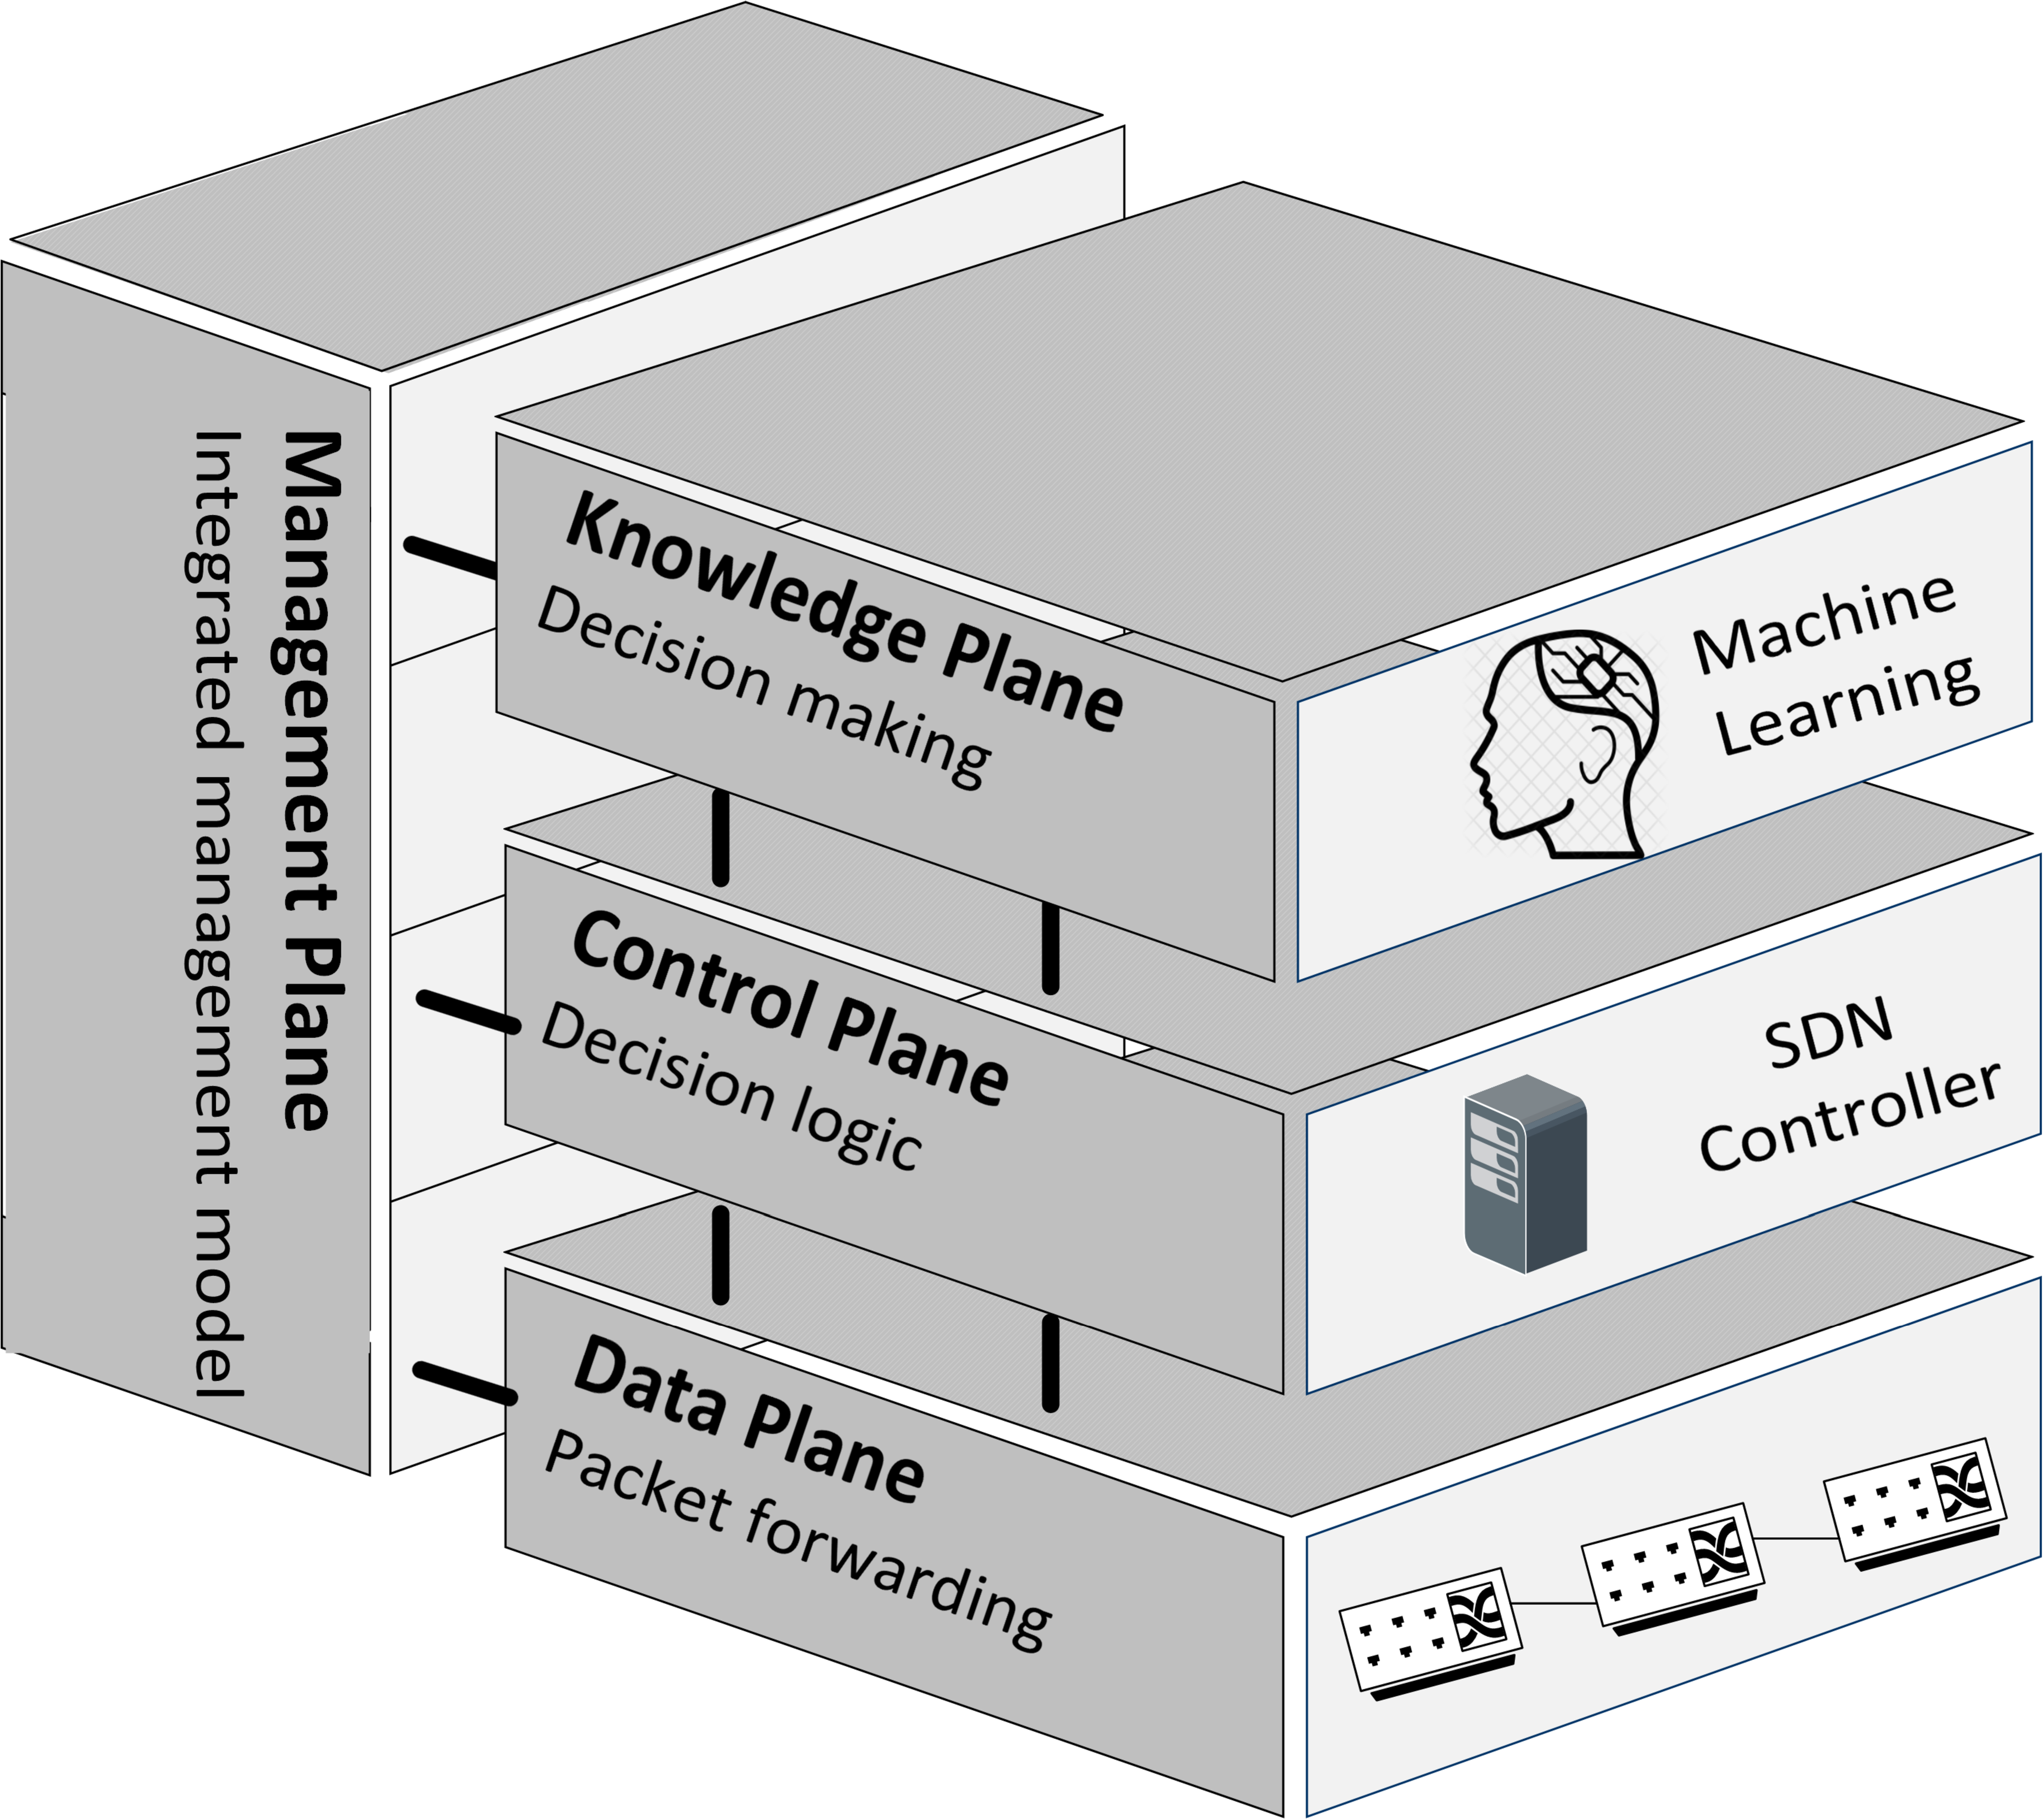
\includegraphics[scale=0.1]{figures/Figure1-KDN-architectured-3d.pdf}
    \caption{High-level KDN architecture (adapted from \cite{mestres_2017:KDN})}
    \label{fig:kdn_architecture}
\end{figure}

\begin{itemize}
    \item The DP is composed of network devices of programmable forwarding and is responsible for storing, forwarding and processing data packets. This plane depends on the CP and MP planes to populate the forwarding tables and update their configuration.
    
    \item The CP translates the requirements from the KP and AP in a specific network policy. Subsequently, CP is based on this policy to update and program matching and processing rules from the DP forwarding elements by SBI.
    
    \item The MP, as well as CP, ensures the correct operation and performance of the network in the long term. It defines the network topology and handles the provision and configuration of network devices. MP generates Metadata with information about the network state, events, statistical metrics per flow and per switch (\textit{e.g.}, packet loss, link failure, memory usage, and CPU utilization). The Metadata is sent to CP and KP. CP handles events that require immediate action (\textit{e.g.}, link failure, black-hole or loop detection). KP handles events that require knowledge (\textit{e.g.}, resource planning, optimization, performance management, and verification).
    
    \item The KP leverages MP and CP to obtain a rich view and control over the network. It is responsible for learning the behavior of the network and, in some cases, automatically operate the network accordingly. Fundamentally, the KP processes the Metadata generated by the MP, transforms them into knowledge via ML, and uses that knowledge to make decisions (either automatically or through human intervention). It is important to mention that, KP is separated from CP because ML algorithm is generally compute-intensive and it may affect the performance of the control plane.

\end{itemize}

This master dissertation supposes that RL is a technique useful to maintain MA and decrease the overhead of monitoring in SDN because it allows optimizing the probing interval by interacting with the network itself (\textit{i.e.,} environment in RL terms).\\

%It is to highlight that in \cite{mestres_2017:KDN}, the authors argue that KDN can be used to carry out intelligent network monitoring. It is because KDN would provide optimization, recommendation, and automation in the process of making decisions focused on improving the network behavior.
%\textbf{Knowledge-Defined Networking} encourages the use of ML to change the way the network operators handle, optimize and troubleshoot SDN \cite{mestres_2017:KDN}. In particular, By using ML techniques, it is possible to learn from the network behavior to provide automation (recognize-act) and recommendations (recognize-explain-suggest) that support management tasks. In turn, SDN offers full control and a network-wide view from a logically centralized point (\textit{i.e.}, controller). In this master dissertation, we argue that Reinforcement Learning (RL) is an ML technique useful to maintain MA and decrease the overhead of monitoring in SDN because it allows optimizing the probing interval by interacting with the network itself (\textit{i.e.,} environment in RL terms).

\subsection{Reinforcement Learning}
\label{subsec:background-rl}
In RL, an agent learns a decision-making process by interacting with an environment \cite{sutton_1998:rl}. Formally, in RL, the environment is typically modeled as a finite Markov Decision Processes (MDP) \cite{kolobov2012:markov} where the agent sends actions and receives outputs (observations and rewards). In a finite MDP, the agent and environment interact at discrete time steps $t = 0, 1, 2,..., N$. At each time-step $t$, the agent receives some representation of the state of the environment, ${S}_t \in S $, where $S$ is the set of possible states. Based on ${S}_t $, the agent selects an action, ${A}_t \in A(S_t) $, where $ A(S_t) $ is the set of available actions in the state ${S}_t $. The execution of action $A_{t}$ puts the agent into the new state $S_{t+1}$. Furthermore, the agent receives a numerical reward from the environment, $R_{t+1} \in  \mathbb{R}$ at step $t \in N$. Then, the total reward that the agent receives over its lifetime for this particular behavior is:

{\setlength{\mathindent}{6cm}
\begin{equation}
    \begin{split}
        U\left ( s \right ) = \sum_{t=0}^{\infty} \gamma^{t}R_{t}
    \end{split}
    \label{equ:total-reward}
\end{equation}
}
where $\gamma \in \left ( 0,1 \right ]$ is called the discount factor. If $\gamma < 1$, the discounting is used. Otherwise, it is not used. \\

RL algorithms find an optimal policy $ \Pi^{*}: S \rightarrow A $ that maximizes the expected cumulative reward for every state, using the exploration methods (\textit{e.g.}, $\varepsilon$-greedy, Boltzmann \cite{sutton_1998:rl} \cite{teng_2012:exploration}). The main RL features are its capacity to run without any prior knowledge of the environment (here, the monitored network) and make its own decisions in execution time (on-line). Nonetheless, RL requires a training period to capture the environment model before converging to the optimal policy.\\

\textbf{Q-learning} is one of the most important RL techniques \cite{duryea_2016:exploring_qlearning} because:

\begin{itemize}
    \item It was the pioneering RL method used for control purposes.
    \item It has a learning curve that tends to converge quickly.
    \item It is the simplest technique that directly calculates the optimal action policy without an intermediate cost evaluation step and without the use of a model \textit{(i.e.}, model-free).
    \item It has an off-policy learning capability; this means, the agent can learn an optimal policy (called Q-function), even if it does not always choose optimal actions. The only condition is that the agent regularly visits and updates all the $(S_t, A_t)$ pairs.
\end{itemize}{}

It is important to highlight that there are other RL strategies, such as Adaptive Heuristic Critic (AHC), Model-free Learning With Average Reward, and some Q-learning variations \cite{manju_2011:analysis_ql} \cite{kaelbling_1996:reinforcement}. These strategies are out of the scope of this master dissertation.\\

Q-learning \cite{Watkins:1989:q_learning} \cite{farahnakian_2011:q-learning} relies on an optimal action-value function $ Q_{t}(S_t,A_t)$, called Q-function. In this function, the value is the estimated reward of executing an action $A_t$ in the state $S_t$, assuming that the agent will follow the policy that provides the maximum reward. Q-learning starts with an arbitrary Q-function $Q_{0}$. At any state $S_{t}$, an agent selects an action $A_{t}$ that determines the transition to the next state $S_{t+1}$ and with the value associated to the pair ($S_t,A_t$) adjusts the values of Q-function according to:

{\setlength{\mathindent}{2cm}
\begin{equation}
    \begin{split}
        Q_{t+1}(S_t,A_t) \leftarrow & (1-\alpha) \cdot Q_{t}(S_t,A_t) + \alpha \cdot \left [R_{t+1} + \gamma \cdot \underset{\rm A}{\rm max} Q_{t}(S_{t+1},A) \right]
    \end{split}
    \label{equ:q_function}
\end{equation}
}

where $R_{t+1}$ denotes the reward received at time $t+ 1$, $\alpha \in \left [ 0,1 \right ]$ is the learning factor (a small positive number) that determines the importance of the acquired reward. A factor $\alpha = 0$ makes the agent does not learn from the latest ($S_t,A_t$) pair. In turn, a factor $\alpha = 1$ makes the agent considers the immediate rewards without taking into account the future rewards. $\gamma \in \left [ 0,1 \right ]$ is the discount factor that determines the importance of future rewards. A factor $\gamma = 0$ prohibits the agent from acquiring future rewards. A factor $\gamma = 1$ forces the agent only to consider future rewards. The part between square brackets is the updated value that represents the difference between the current estimate of the optimal Q-value $Q_t(S_t,A_t)$ for a state-action pair ($  S_{t}, A_{t} $), and the new estimate $ \left [R_{t+1} + \gamma  \underset{\rm A}{\rm max} Q_t(S_{t+1},A) \right ]$.\\

The Q-function approximates the optimal state-action value function $ Q^*$ regardless of the followed policy. It is noteworthy that the updated Q-function $Q_{t} $ only depends on the previous function $Q_{t-1} $ combined with the experience ($S_{t}, A_{t}, R_{t}, S_{t+1}$). Thus, Q-learning is both computationally and memory efficient. Nonetheless, if the number of states is high, Q-learning may take much time and require more data to converge (\textit{i.e.,} find the best action for each state). Therefore, in Q-learning is critical to have a concise representation of the environment (\textit{i.e.,} the network model).\\

To find the Q-function, Q-learning requires an exploration method. The exploration method selects an action to perform at each step, which represents the Q-function. $\varepsilon$-greedy exploration is one of the most used exploration methods \cite{teng_2012:exploration} \cite{Tijsma_2016:exploration_q_learning}. It uses $\varepsilon \in \left [ 0,1 \right ]$ as the parameter of exploration to decide which action to perform using $Q_{t}(S_{t},A)$. With this parameter the action is as follows:

{\setlength{\mathindent}{4cm}
\begin{equation}
    \begin{split}
       \mathcal{A} = \begin{Bmatrix}
            \underset{\rm A}{\rm max} Q_{t}(S_{t},A) & with \thinspace probability\thinspace 1-\varepsilon \\ 
            random\thinspace action & with\thinspace probability \thinspace \varepsilon
        \end{Bmatrix}
    \end{split}
    \label{equ:e-greedy}
\end{equation}
}

$\varepsilon$-greedy exploration method adds some randomness when deciding between actions. Instead of always selecting the best available action, this method randomly explores other actions with a probability = $\varepsilon$ or chooses the best action (highest Q-value) with a probability = $1-\varepsilon$. A high value for $\varepsilon$ adds randomness to the exploration method, which will make the agent explores other actions more frequently. Randomness is necessary for an agent to learn the optimal policy.
\section{Overview}
\label{sec:Overview}
\begin{figure*}[h!]
    \centering
    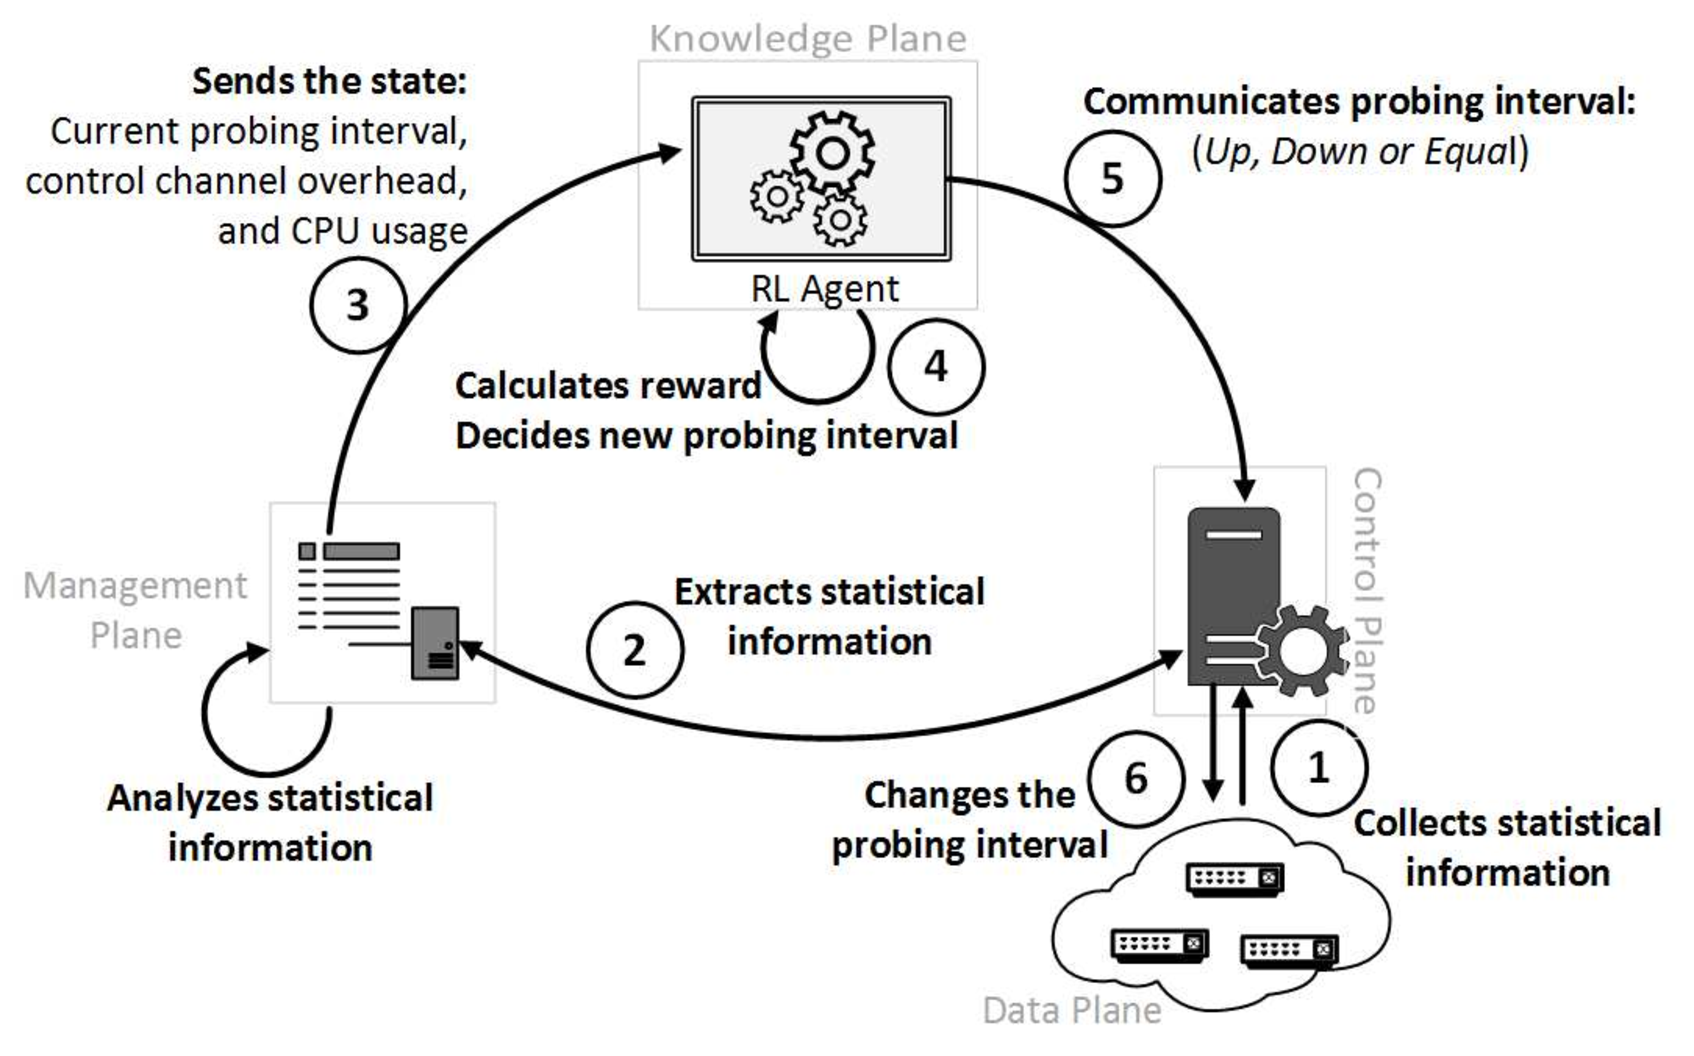
\includegraphics[width=0.75\textwidth]{figures/Figure2-IPro-high-level-operation}
    \caption{IPro - High-Level Operation}
    \label{fig:high_level_ipro}
\end{figure*}

IPro applies RL to optimize the probing interval regarding to CCO and CUC. Figure~\ref{fig:high_level_ipro} depicts how IPro operates in a high-abstraction level:

\begin{enumerate}[label=\protect\circled{\arabic*}]
    \item The Control Plane (CP) collects statistical information from the Data Plane (DP) at some probing interval. Since this collection of information affects the network behavior, the network falls in a new state.
    \item The Management Plane (MP) extracts these statistics to determine such a new state by analyzing CCO and CUC.
    \item MP sends this new state to the Knowledge Plane (KP).
    \item The RL-agent takes such a state to calculate the reward. It is important to highlight that a low reward indicates high CCO and high CUC. Based on the reward, the RL-agent decides a new probing interval intended to minimize CCO and CUC.
    \item The RL-agent communicates this new probing interval to CP.
    \item The CP applies this interval that affects the network behavior again. This operation continues until the network administrator decides to stop IPro.
\end{enumerate}

%\circled{1} the Control Plane (CP) collects statistical information from the Data Plane (DP) at some probing interval. Since this collection of information affects the network behavior, the network falls in a new state. \circled{2} the Management Plane (MP) extracts these statistics to determine such a new state by analyzing CCO and CUC. Subsequently, in \circled{3}, MP sends this new state to the Knowledge Plane (KP). In \circled{4}, the RL-agent takes such a state to calculate the reward. It is important to highlight that a low reward indicates high CCO and high CUC. Based on the reward, the RL-agent decides a new probing interval intended to minimize CCO and CUC. \circled{5} the RL-agent communicates this new probing interval to CP. In \circled{6}, CP applies this interval that affects the network behavior again. This operation continues until the network administrator decides to stop IPro.

\section{Architectural Layers and Elements}
\label{sec:detailed_architecture}

Figure~\ref{fig:detail_ipro} introduces and details the IPro architecture. IPro has four main planes that follow the KDN fundamentals. Next, these plans are detailed.

\begin{figure}[h!]
    \centering
    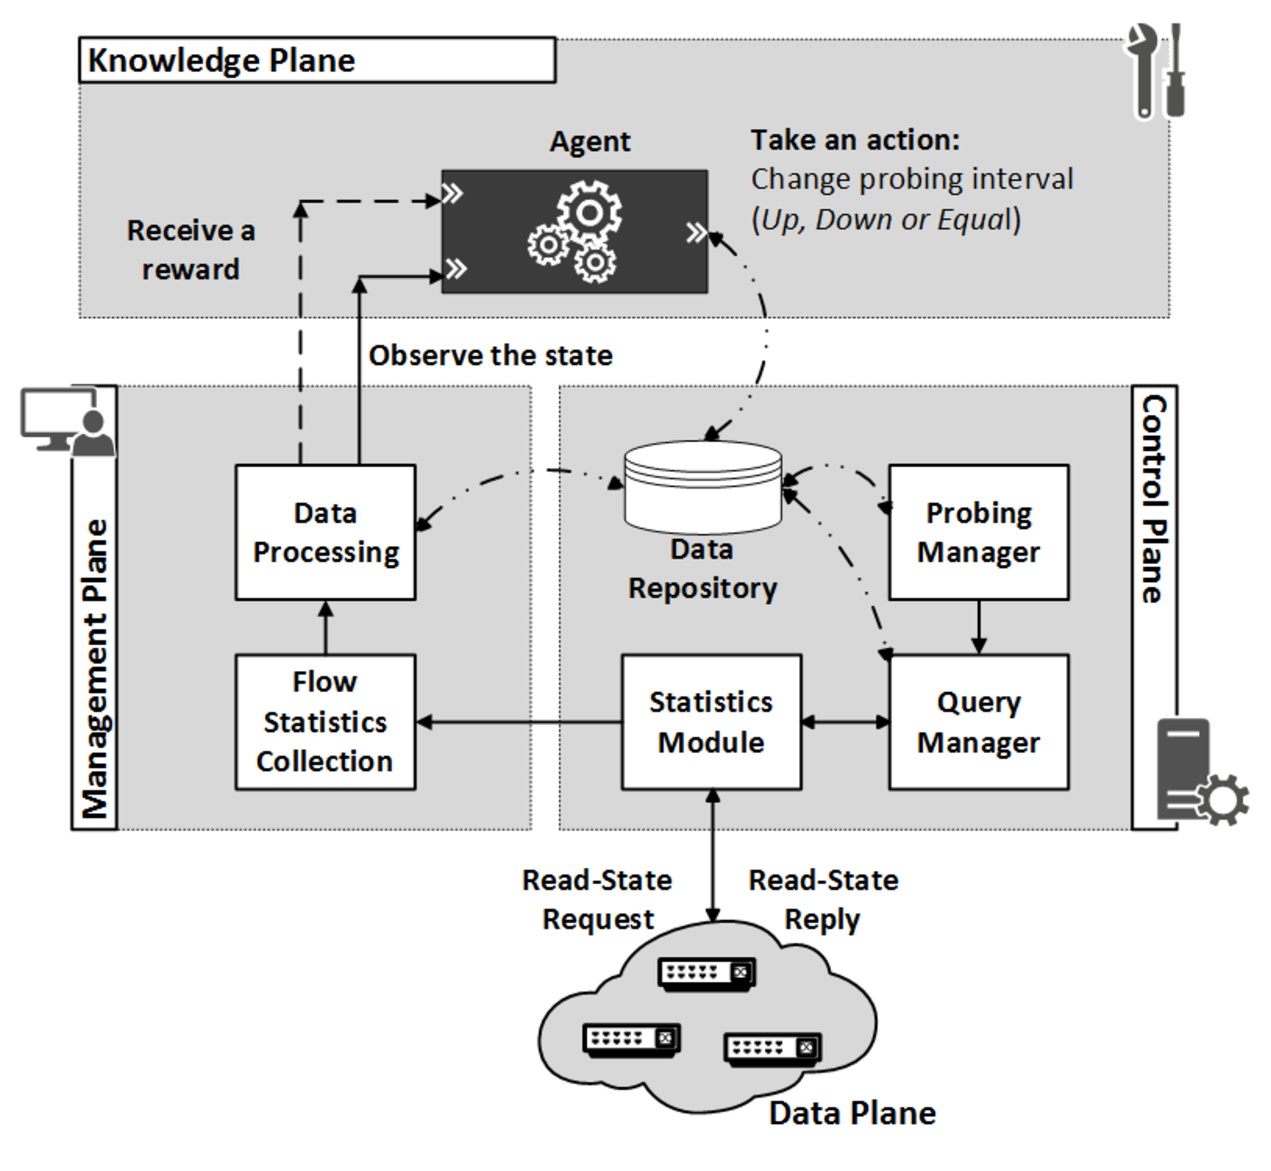
\includegraphics[width=0.60\columnwidth]{figures/Fig2-IPro-architecture}
    \caption{IPro Architecture}
    \label{fig:detail_ipro}
\end{figure}

%\paragraph{\textbf{Knowledge Plane.}}
\subsection{Knowledge Plane}
This plane obtains a rich view and global control over the network from MP and CP. Overall, KP operates in three steps:
\begin{itemize}
    \item It organizes the metadata generated by MP.
    \item It converts that metadata into knowledge by using ML techniques.
    \item It uses that knowledge to make decisions (either automatically or through human intervention) related to routing, traffic classification, anomalies detection, and so on. 
\end{itemize}{}

It is essential to highlight that KP is separated from CP because ML algorithm is generally compute-intensive, and it may affect the performance of CP \cite{mestres_2017:KDN}. In this master dissertation, KP is responsible for learning the network behavior and automatically deciding a new probing interval. KP obtains the current network status and controls the probing interval by interacting with MP and CP, respectively. The KP heart is the RL-agent. This agent is in charge of determining the most-rewarding probing strategy intended to maintain CCO and CUC within target values. IPro considers two thresholds $\omega$ and $\chi$ that are configurable according to network requirements. $\omega$ represents the policy 1 and aims at preventing a high CCO. In turn, $\chi$ represents the policy 2 and aims at preventing a high CUC. To sum up, the RL-agent handles the monitoring policies by controlling $\omega$ and $\chi$. \\

Control policies are defined to prevent monitoring messages from affecting the performance of the controller and the bandwidth of the control channel. For instance, when CUC exceeds 80\% of the CPU capacity, the controller increases its response time, which generates delays and loss \cite{repas_2015:performance_cpu}. In the same sense, when the use of the control channel bandwidth exceeds 80\%, the monitoring messages can interfere with the SDN functions \cite{xu_2017:wildcard_requests}.\\

\begin{figure}[h!]
    \centering
    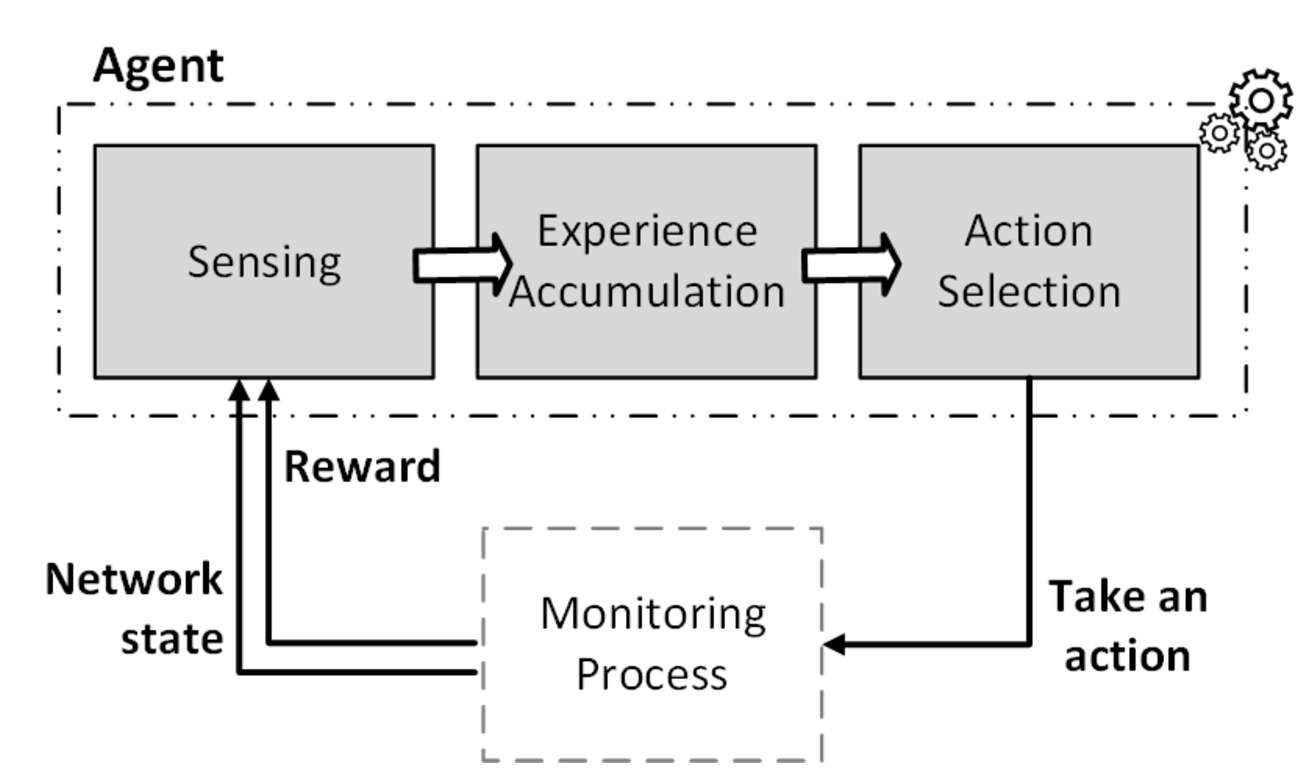
\includegraphics[width=0.50\columnwidth]{figures/Fig3-IPro-agent}
    \caption{The RL-agent General Model}
    \label{fig:ipro_agent}
\end{figure}

Figure~\ref{fig:ipro_agent} depicts the general model of the RL-agent. This model includes three elements, namely, \textit{Sensing}, \textit{Experience Accumulation}, and \textit{Action Selection}. \textit{Sensing} enables the RL-agent to get the network state and the reward of the IPro monitoring process. The \textit{Experience Accumulation} element guides the policy (i.e., what action to take) of the agent in two steps. In the first one, this element combines the observations made by \textit{Sensing} and defines the information matrix that represents the internal states of the RL-agent. In the second step, \textit{Experience Accumulation} maps these states and assigns rewards to indicate how good or bad these states are according to the accumulated experience. \textit{Action Selection} guides the action policy considering the most-rewarding probing strategy based on the current network state. Section~\ref{sec:ipro_algorithm} depicts the detailed procedure carried out by the RL-agent.

\subsection{Control Plane}
This plane translates the requirements from KP and the Application Plane (AP) in specific network policies. CP uses such policies to update and program matching and processing rules in DP forwarding elements via a SBI, such as OpenFlow \cite{onf_2012:openflow}, Forwarding and Control Element Separation (ForCES) \cite{doria_2010:forces}, and Protocol-Oblivious Forwarding (POF) \cite{song_2013:POF}. \\

In this master dissertation, CP handles network monitoring by performing the steps described in Algorithm 1. 

\begin{itemize}
    \item CP receives decisions about the new probing interval ($I$) from KP.
    \item CP applies these decisions to handle the data collection in the monitored network.
    \item CP sends Read-State request messages to each switch connected (line 3) to this plane every $I$ seconds (line 5).
    \item CP receives the Read-State reply messages asynchronously (line 6), which contain the statistical information from the switches.
    \item CP stores the statistical information (line 7) to maintain a trace of network changes. These steps are repeated indefinitely up to reach a stop criterion (\textit{e.g.,} errors and administrator).
\end{itemize}{}

\newlength{\commentWidth}
\setlength{\commentWidth}{7cm}
\newcommand{\atcp}[1]{\tcp*[r]{\makebox[\commentWidth]{#1\hfill}}}
\begin{english_algorithm}
\footnotesize
\SetAlgoLined
\SetKwInOut{Input}{Require}
\SetKwInOut{Output}{Output}

\Input{
    \\
    Probing interval $I$ \\
}
%\KwResult{A probing interval}
\BlankLine
   \While{not reached stopping criterion}{
       \ForEach{$switch \in switches$}{
            Send a Read-State Request message to $switch$
        }
        Wait for $I$ seconds\\
        Receive the Read-State Reply Messages from the switches \tcp*[h]{These messages contain the statistical information}\;
        Store the statistical information
    }
%}
%\Return $Q$
%\caption{$Q$-learning: Learn Function $Q: \mathcal{S} \times \mathcal{A} \rightarrow \mathbb{R}$}
\label{alg:ipro_collection}
\caption{Data Collection}
\end{english_algorithm}

CP includes four elements namely, \textit{Probing Manager, Query Manager, Statistics Module, and Data Repository}. 

\begin{itemize}
    \item \textit{Probing Manager} sets up the probing interval according to the decision made by the RL-agent.
    \item  \textit{Query Manager} handles the data collection based on the computed probing interval and the desired aggregation levels (\textit{e.g.}, byte, packet, flow). After this data collection, \textit{Query Manager} merges and stores the statistical information into the data repository. Thus, this information can be used ulteriorly by upper-layer applications.
    \item \textit{Statistics Module} is a service running on the top of the SDN controller, which is useful to develop customized network measurement applications.
    \item \textit{Data Repository} stores statistical information of each monitoring operation and maintains a trace of network changes.
\end{itemize}{}

It is important to highlight that CP interacts with KP by a Data Repository.

\subsection{Management Plane}
This plane ensures that the network as a whole is running optimally carrying out the Operation, Administration, and Maintenance (OAM) functions \cite{wickboldt_2015:management_requeriments,denazis_2015:layer_architecture}. MP defines the network topology and handles the provision and configuration of network devices. Furthermore, it generates metadata with information about the network state, events, statistical metrics per-flow, and per-switch (\textit{e.g.}, packet loss, link failure, memory usage, and CPU utilization). \\

In this master dissertation, this plane is responsible for extracting the statistical information from CP to provide an analysis of the network state to KP regarding CCO and CUC. MP includes two elements called, \textit{Flow Statistics Collection and Data Processing}. The first one extracts the statistical information from \textit{Statistics Module} located at CP. The second element is responsible for processing and organizing the information retrieved by \textit{Flow Statistics Collection} to compute CCO and CUC. \textit{Data Processing} also sends the processed information to the RL-agent located at KP while keeps a historical record of the network state into \textit{Data Repository}.\\

It is noteworthy that MP interacts with CP by a REST-based interface. In turn, MP communicates with KP by specific APIs since, up to now, there are no standardized interfaces for KP.

\subsection{Data Plane}
This plane is responsible for forwarding flows in the monitored SDN by network devices decoupled from CP \cite{varghese2005network}. Each network device consists of a physical part and a functional part. The physical part comprises hardware elements, such as ports, storage, processor, and memory. The functional part comprises a limited set of operations, such as packet header parsing and extraction of a header field tuple, support for a fixed set of packet operations (such as header field manipulation and forwarding through a specific set of ports), and the ability to match packet header tuples against a lookup memory primitive (\textit{e.g.}, a hash table or a content addressable memory).\\

It is important to mention that, in SDN, it is key to perform intelligent monitoring decisions, by MP, CP, and KP, aiming at improving the network performance \cite{kreutz_2015:sdn_comprehensive_survey,isolani_2015:interactive, mestres_2017:KDN}.

% Reconfigurable Network Systems and Software-Defined Networking
% mscThesis--Network Monitoring with Software Defined Networking
\section{Probing Algorithm}
\label{sec:ipro_algorithm}

\subsection{Assumptions}
\label{subsec:assumptions}

\subsubsection{Reward}
It defines the objective of any RL-agent. In IPro, the reward targets to ensure the accomplishing of network policies regarding CCO and CUC. Let us consider that the RL-agent chooses an action and increases the probing interval. If IPro does not meet with one or more policies (\textit{e.g.,} policy 1 or policy 2), the RL-agent will learn that it is a wrong action; resulting in a negative reward. Conversely, if IPro meets the policies, the RL-agent will learn that such an increase is a good action; resulting in a positive reward.\\

One of the main RL challenges is to define the reward function. In some cases, the choice of this function is easy because it is implicit in the task. For instance,  in an Atari game, there is a score function that is part of the game itself. In other cases, like in IPro, the choice of such function is complex. The RL-agent has a task objective with multiple criteria, such as keeping CCO and CUC within target values to minimize network performance degradation. In the proposed approach, these criteria are combined in a single scalar-valued reward function using the normal distribution defined by Matignon \textit{et al.} \cite{matignon_2006:improving}, whose heuristic allows defining a multi-objective model useful to consider CCO and CUC (control policies) simultaneously. Therefore, the reward function is defined as follows.

{\setlength{\mathindent}{4cm}
\begin{equation}
    \begin{split}
       R\left ( S_t, A_t \right ) = \beta_c e^{-\frac{d\left ( C\left ( \Theta  \right ), C\left ( \Theta  \right )* \right )^2}{2\sigma_c^2 }} + \beta_u e^{-\frac{d\left ( Us,Us* \right )^2}{2\sigma_u^2 }}
    \end{split}
     \label{equ:reward}
\end{equation}
}

where, $\beta$ adjusts the amplitude of the function and $\sigma$, the standard deviation, specifies the reward gradient influence area. $d$ is the Manhattan distance between the new state $s$ and goal state $s*$. $\Theta$ is the set of active flows in the network. $C\left ( \Theta  \right ) $ and $C\left ( \Theta  \right )*$ are the CCO (cf. equation \ref{equ:load}) used for statistics collection of the set of flows $\Theta$ from the switches in states $s$ and $s*$, respectively. $Us$ and $Us*$ are CUC in states $s$ and $s*$, respectively.\\

\subsubsection{Space of Actions}
The space of actions affects the future state of the network (e.g., the next CCO and CUC), changing the options and opportunities available to the RL-agent at later times. The effects of actions cannot be fully predicted; thus, the RL-agent must monitor the network frequently and react appropriately (i.e., search process). For example, it must watch the probing interval to avoid the breach of policies.

\newlength{\commentWidth}
\setlength{\commentWidth}{7cm}
\newcommand{\atcp}[1]{\tcp*[r]{\makebox[\commentWidth]{#1\hfill}}}
\begin{english_algorithm}
\footnotesize
\SetAlgoLined
\SetKwInOut{Input}{Require}
\SetKwInOut{Output}{Output}

\BlankLine
    \uIf {$action=increase$}{
        Increases the current probing interval}
    \uElseIf{$action=reduce$}{
        Decreases the current probing interval}
    \Else{
        Keeps the current probing interval
      }
\label{alg:actions_algorithm}
\caption{Space of Actions}
\end{english_algorithm}

The RL-agent performs the search process using the action functions (increase, reduce, and keep) in Algorithm 2 to change the probing interval in each iteration and uses the reward function as the guide to the goal state.

\subsubsection{Space of States}
The space of states represents a signal transferring to the agent some sense of ``how the network is'' at a particular time. This space is represented as follows:

{\setlength{\mathindent}{6cm}
\begin{equation}
   % \begin{split}
      S\equiv f \left ( i, l, cpu \right )
%    \end{split}
    \label{equ:states_model}
\end{equation}
}

Each $S_t= \left ( i_t, l_t, cpu_t \right ) \in S$ is characterized by the probing interval $i_t$, CCO $l_t$, and CUC $cpu_t$ in the time $t$. CCO corresponds to the bandwidth consumed by IPro when transmitting and receiving Read-State messages between CP and DP. CUC defines the number of instructions carried out in CP because of IPro tasks (\textit{e.g.}, RL-agent execution, processing of data collection messages). The probing interval indicates how often CP must send Read-State Request messages to retrieve flow statistics from switches in DP.

\subsubsection{Statistics Collection} 
In SDN, the pull-based monitoring is handled by the controller that interacts with the switches via a control channel over TCP. There are two interaction methods \cite{xu_2017:wildcard_requests} \cite{su_2015:cemon}: Per-Flow Collection (PFC) and Per-Switch Collection (PSC). 

\begin{itemize}
    \item In PFC, the controller sends a request to a switch to collect the traffic statistics of one particular flow. This method generates a high CCO when the controller requires to collect statistics of many flows. This overhead is due to the large quantity of Read-State Request messages sent per switch.
    \item In PSC, the controller sends a request to collect the traffic statistics of all flow entries from a switch. This method reduces the number of Read-State Reply messages (Controller$<->$Switch) and, so, reduces CCO and CUC. Nonetheless, if PSC is used excessively with, for instance, a low probing interval, it can cause flow statistics overlapping, high CCO, and high CUC. %In IPro, we use PSC because it allows tuning the probing interval to handle CCO and CUC efficiently.
\end{itemize}{}

This master dissertation focuses on the PSC method because first, PSC generates a smaller amount of Read-State messages that imply lower CCO and CUC. Second, PSC reduces the repeated headers of the flows that involve less redundancy in the collected information \cite{su_2015:cemon}.\\

In IPro, the \textbf{SDN Model} consists of a logically-centralized controller (may be a cluster of distributed controllers \cite{jose_2011:online_measurement} \cite{tahaei_2018:distributed_controller}) and a set of switches. The SDN is modeled by an out-of-band control plane and an undirected graph $G=(V,E)$, where $V=\left \{ v_1,..., v_n \right \}$ is the set of nodes (switches and controllers) and $E=\left \{ e_1,..., e_u \right \}$ is the set of links connecting nodes. This master dissertation assumes that the controller knows the existing active flows in the network, denoted by $\Theta = \left \{ \theta_1, \theta_2, ..., \theta_m \right \} $, with $m=\left | \Theta  \right |$. Thus, it is also reasonable to assume that the controller knows each flow that passes through each switch $v_i$, denoted by $\theta_i$, with $i=1,2,...,m$. Therefore, the active flows number in switch $v_i$ is $\left | \theta_i  \right |$. It is noteworthy that the evaluation of CCO and CUC is critical for any out-of-band CP because, first, the control bandwidth is a limited resource and must be analyzed and optimized. Second, CUC is also a constrained resource that must be used appropriately to avoid the wrong behavior of CP and, so, of the underlying DP.

\subsubsection{Control Channel Overhead} 
CCO is the bandwidth cost used for statistics collection of a set of flows from the switches. In IPro, the controller generates this cost when requests and receives to and from the switches the statistics of a set of flows $\theta_i$. According to \cite{onf_2012:openflow}\cite{su_2015:cemon}, the bandwidth cost caused by $\theta_i$ involves two parts: (\textit{i}) the size of the Read-State Request messages $l_{rq}$ sent to switches; and (\textit{ii}) the size of the Read-State Reply messages  $l_{rp}$ that depends on the number of existing flows $\left | \theta_i  \right |$ in the flow tables. Thus, the bandwidth cost is defined as follows.

{\setlength{\mathindent}{4cm}
\begin{equation}
    C\left ( \Theta  \right ) = l_{rq} \cdot \left | V \right | + l_{rp} \cdot \sum_{i=1}^{\left | V \right |} \left | \theta_i \right |, \forall i \leqslant \left | V \right |
    \label{equ:load}
\end{equation}
}

\subsubsection{CPU Usage of the Controller}
CUC is the number of instructions generated by execution, calculation, and comparison of raw data in IPro. According to \cite{tahaei_2018:distributed_controller}, CUC can be estimated through a constant ($x$) that indicates the number of instructions carried out by CPU to fragment the Read-State Reply messages. Therefore, CUC for analyzing $n$ specific flows from $\Theta$ is modeled as a linear function of $n$.

{\setlength{\mathindent}{3cm}
\begin{equation}
    CPU \cong \left | V \right |* n\left ( ReadStateReply \right ) * x,  \forall n \in \Theta
     \label{equ:load_cpu}
\end{equation}
}
\subsubsection{Monitoring Accuracy} 
MA reflects the difference between the real value of a metric and the measured value by IPro. A smaller difference (error) indicates a higher MA. The error is calculated with the following expression:

{\setlength{\mathindent}{5cm}
\begin{equation}
    \begin{split}
        \%error = \frac{\left | v_{C}-v_{R} \right |}{v_{R}}*100
    \end{split}
     \label{equ:percent-error}
\end{equation}
}
where, $v_{C}$ is the measured value of the metric being monitored and $v_{R}$ is the real value (or reference). Therefore, MA is as follows:
{\setlength{\mathindent}{5cm}
\begin{equation}
    \begin{split}
        MA = 100\% - \%error
    \end{split}
     \label{equ:ma}
\end{equation}
}

\subsection{Functioning}
\label{subsec:assumptions}

Algorithm 3 presents the probing interval optimization procedure carried out by IPro. The algorithm inputs are the learning factor $\alpha$, the discount factor $\gamma$ (\textit{cf.} Equation~\ref{equ:q_function}), and the exploration method $\varepsilon$ (cf. Equation~\ref{equ:e-greedy}). The output is the most-rewarding probing interval according to the current network status.\\

The probing algorithm has two considerations: \textit{i}) it assumes a null initial condition of the $Q(\mathcal{S},\mathcal{A})$ before the first update occurs (line 1); and \textit{ii}) it starts its execution from a random state that represents the initial values of probing interval, CCO, and CUC (line 3). After these considerations, the probing interval optimization process begins (line 4). In this process, the RL-agent discovers the reward structure and determines the most-rewarding probing interval by interacting with the network. The proposed algorithm performs the following steps in each iteration (lines 5 to 13):

\newlength{\commentWidth}
\setlength{\commentWidth}{7cm}
\newcommand{\atcp}[1]{\tcp*[r]{\makebox[\commentWidth]{#1\hfill}}}
\begin{english_algorithm}
\footnotesize
\SetAlgoLined
\SetKwInOut{Input}{Require}
\SetKwInOut{Output}{Output}

\Input{
    \\
    %States $\mathcal{S} = \{1, \dots, n_s\}$ \\
    %Actions $\mathcal{A} = \{1, \dots, n_a\},\qquad A: \mathcal{S} \Rightarrow \mathcal{A}$ \\
    %Actions $\mathcal{A} = \{up, down, equal\},\qquad A: \mathcal{S} \Rightarrow \mathcal{A}$ \\
    %Reward function $R: \mathcal{S} \times \mathcal{A} \rightarrow \mathbb{R}$ \\
    Exploration parameter  $\varepsilon$ \\
    %Transition function ($\epsilon$) $T: \mathcal{S} \times \mathcal{A} \rightarrow \mathcal{S}$ \\
    Discount factor $\gamma$ \\
    Learning factor $\alpha$ \\
    %Reward function $R: (S,A) \rightarrow R $
}
\KwResult{A probing interval}

%Initialize $Current Bandwidth$ $CB$\;
%Calculate current traffic according to Control and Monitoring messages $CM$ \;
%\If{$ CM > CB * 0.8 $}{
\BlankLine
Initialize $Q:$ $Q(\mathcal{S},\mathcal{A})=0, \forall s \in \mathcal{S}, \forall a \in \mathcal{A}$
\BlankLine
    \While{not reached stopping criterion}{
      Start in state $S_{t} \in \mathcal{S}$\;
      %Choose A from $S_{t}$ using policy derived from $\underset{\rm A}{\rm max} Q_{t}(S_{t},A)$\;
        \While{$S_{t}$ is not terminal}{
            Select $A_{t}$ from $S_{t}$ using policy derived from Q using $\varepsilon$-greedy exploration method\;
            %Calculate $\pi$ according to Q \;
            %Exploration strategy (e.g. $\pi(x) \gets \argmax_{a} Q(s, a)$)\;
            $A_{t} \gets \pi(S_{t})$ \tcp*[h]{Execute probing action}\;
            Modify the probing interval according to the action $A_{t}$\;
            $S_{t+1} \gets T(S_{t}, A_{t})$ \tcp*[h]{Receive the new state}\;
            $R_{t+1} \gets R(S_{t}, A_{t})$ \tcp*[h]{Calculate reward}\;
            $Q_{t+1}(S_t,A_t) \leftarrow & (1-\alpha) \cdot Q_{t}(S_t,A_t) +
             &\alpha \cdot \left [R_{t+1} + \gamma \cdot \underset{\rm A}{\rm max} Q_{t}(S_{t+1},A) \right]$\tcp*[h]{Update Q-function}\;
            %Modify the probing interval according to the action $A_{t}$\;
            Send the probing interval modified to Data Repository\;
            $S_{t} \gets S_{t+1}$ \tcp*[h]{Move to the new state}\;
            $t \gets t+1$  \tcp*[h]{Increment and set the number of steps taken}\;
        }
    }
%}
%\Return $Q$
%\caption{$Q$-learning: Learn Function $Q: \mathcal{S} \times \mathcal{A} \rightarrow \mathbb{R}$}
\label{alg:ipro_algorithm}
\caption{Probing Interval Optimization}
\end{english_algorithm}
%\bigskip % add 12pt space in-between

\begin{itemize}
    \item The RL-agent selects a probing action $A_{t}= \{up, down, equal\}$ from the Q-function using the $\varepsilon$-greedy exploration method that modifies the probing interval (line 7). The possible actions are to increase ($up$), reduce ($down$), or keep ($equal$) the probing interval.
    \item The RL-agent executes the probing action selected in the previous step (line 6). Since this execution affects the network behavior, the network falls in a new state. MP determines the new state by Equation~\ref{equ:states_model}, where CCO and CUC are determined using Equation~\ref{equ:load} and Equation~\ref{equ:load_cpu}, respectively. The value of the probing interval is obtained in the step 1. Subsequently, MP sends this new state to the RL-agent.
    \item The RL-agent receives the new network state from MP (line 8). 
    \item The RL-agent takes such a state to calculate the reward (line 9). In particular, the reward is computed by Equation~\ref{equ:reward}.
    \item Based on the learning factor, discount factor, initial considerations, reward, and new network state, the RL-agent tunes the values of the Q-function according to Equation~\ref{equ:q_function} (line 10).
    \item The RL-agent sends the probing interval to \textit{Data Repository} (line 11).
    \item The RL-agent moves to the new state (line 12) and moves on to the next iteration $t+1$ (line 13).
\end{itemize}

The probing interval optimization process is repeated until the agent perceives that the policy does not change. At this moment, the agent gets the most-rewarding probing interval that keeps CCO and CUC within target values aiming at minimizing network performance degradation caused by the monitoring tasks.

\subsection{Computational Complexity}
\label{subsec:computational-complexity}

IPro determines its optimal policy by finding an Optimal Value Function. The Optimal Value Function of a policy is the expected infinite discounted reward that will be gained, at each state, by executing that policy.  This value can be computed by the Equation~\ref{equ:total-reward}, where $Q_{t}(S_{t},A) = E\left ( \sum_{t=0}^{\infty} \gamma^{t}R_{t} \right )$. Once the IPro RL-agent knows the value of each state under the current policy, it considers whether the value could be improved by changing the first action taken. If the value can be improved, the RL-agent changes the policy to take the new action whenever it is in that situation. This step guarantees an improvement in the performance of the policy strictly. When no enhancements are possible, then the policy is optimal.\\

Since IPro operates by successive approximations of an Optimal Value Function, its computational complexity, per iteration, is quadratic in the number of states ($S$) and linear in the number of actions ($A$): ($O\left ( \left | A \right |\left |  S\right |^{2} \right )$). Furthermore, the number of iterations required to reach the Optimal Value Function is polynomial in the number of states and the magnitude of the highest reward if the discount factor is held constant. In the worst case, the number of iterations grows polynomially in $\frac{1}{1-\gamma }$. Thus, the IPro RL-agent convergence rate slows considerably as the discount factor nearby 1.

\subsection{IPro Interactions}
\label{subsec:sequence-diagram}

IPro uses RL to optimize the probing interval regarding CCO and CUC. For higher compression of how the IPro architecture elements interact at run time, the analysis is divided into two general parts: statistics collection process and probing interval optimization process.

\subsubsection{Statistics Collection Process}
\label{subsec:statistics-collection-process}

\begin{figure}[h!]
    \centering
    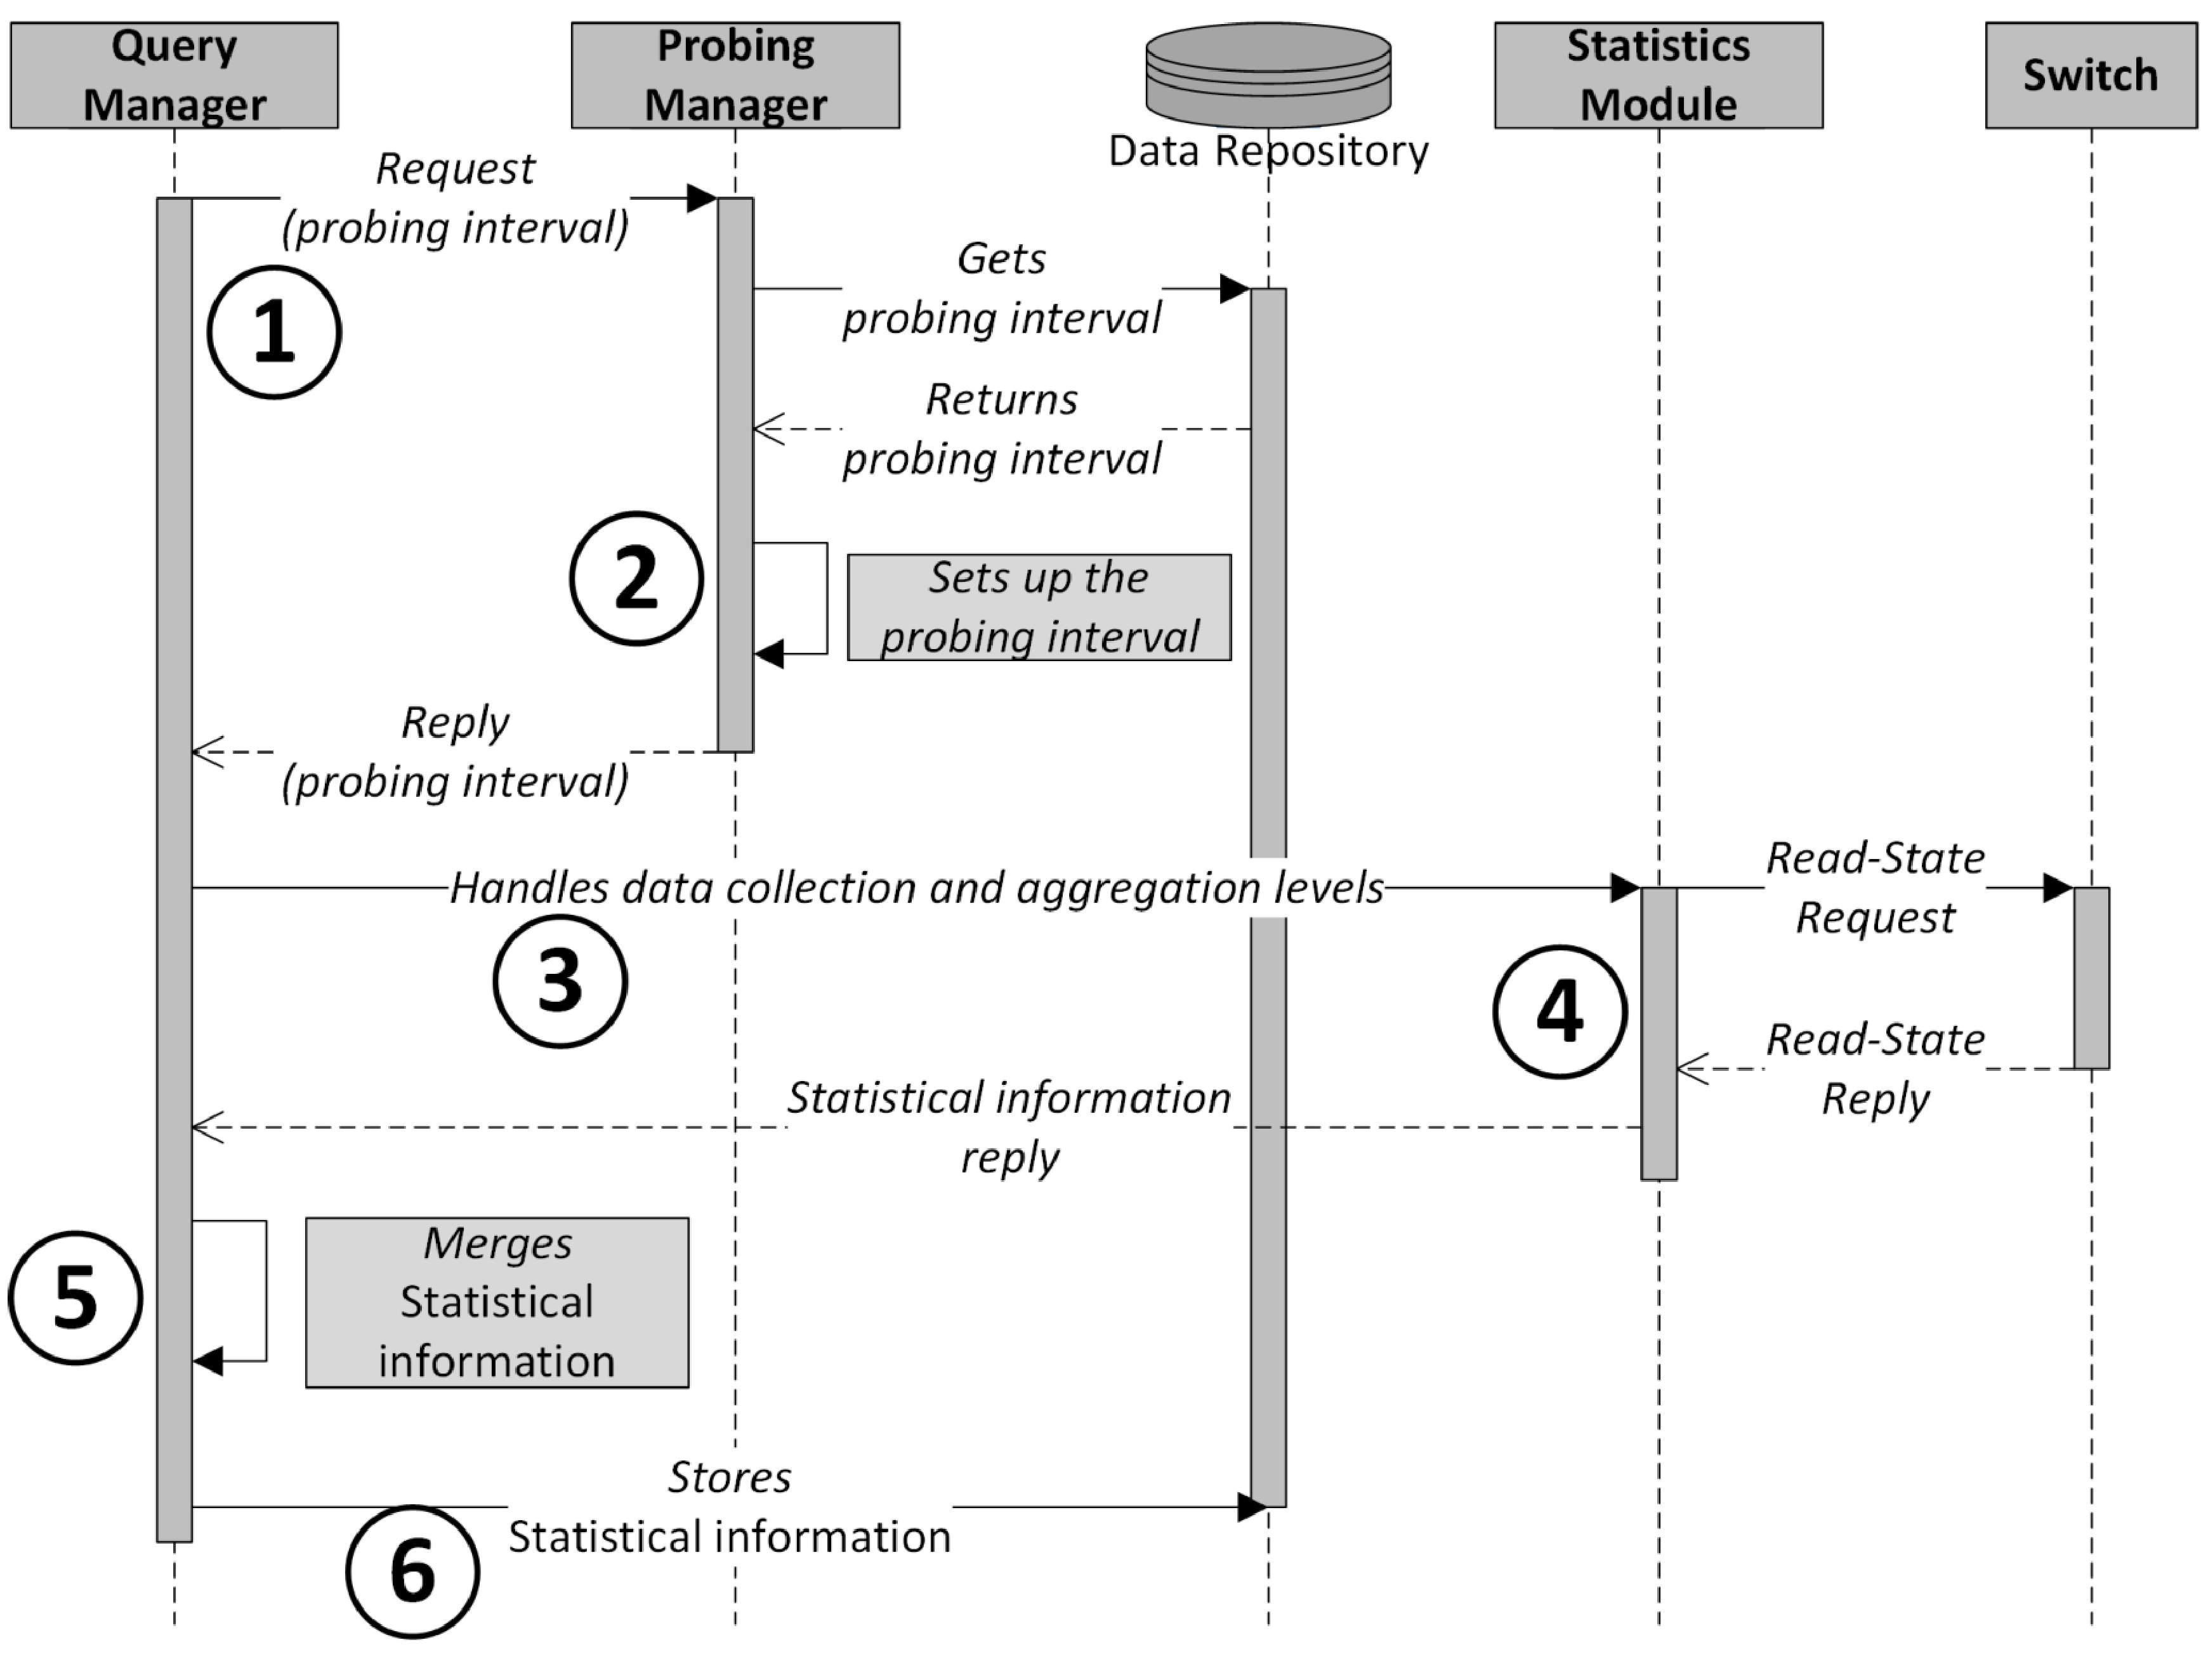
\includegraphics[width=0.90\columnwidth]{figures/Figure5-IPro-Sequence-diagram-cp}
    \caption{Sequence diagram of statistics collection process}
    \label{fig:sequence-diagram-cp}
\end{figure}

Figure~\ref{fig:sequence-diagram-cp} depicts how the elements of CP and DP interact in the statistics collection process. 

\begin{enumerate}[label=\protect\circled{\arabic*}]
    \item Query Manager requests Probing Manager to set up the probing interval to handle the data collection.
    \item Probing Manager consults the data repository to know the probing interval and sets up it how the current interval.
    \item Query Manager handles the data collection based on the current probing interval and the desired aggregation levels (\textit{e.g.}, byte, packet, flow).
    \item Statistics Module collects statistical information from the switch at the current probing interval using Read-State messages (request and reply). After this data collection, Query Manager merges \circled{5} and stores \circled{6} the statistical information into the Data Repository. Thus, this information can be used ulteriorly by upper-layer applications.
\end{enumerate}

It is important to highlight that the collection process affects network behavior; the network falls in a new state.

\subsubsection{Probing Interval Optimization Process}
\label{subsec:probing-interval-optimization-ptocess}

\begin{figure}[h!]
    \centering
    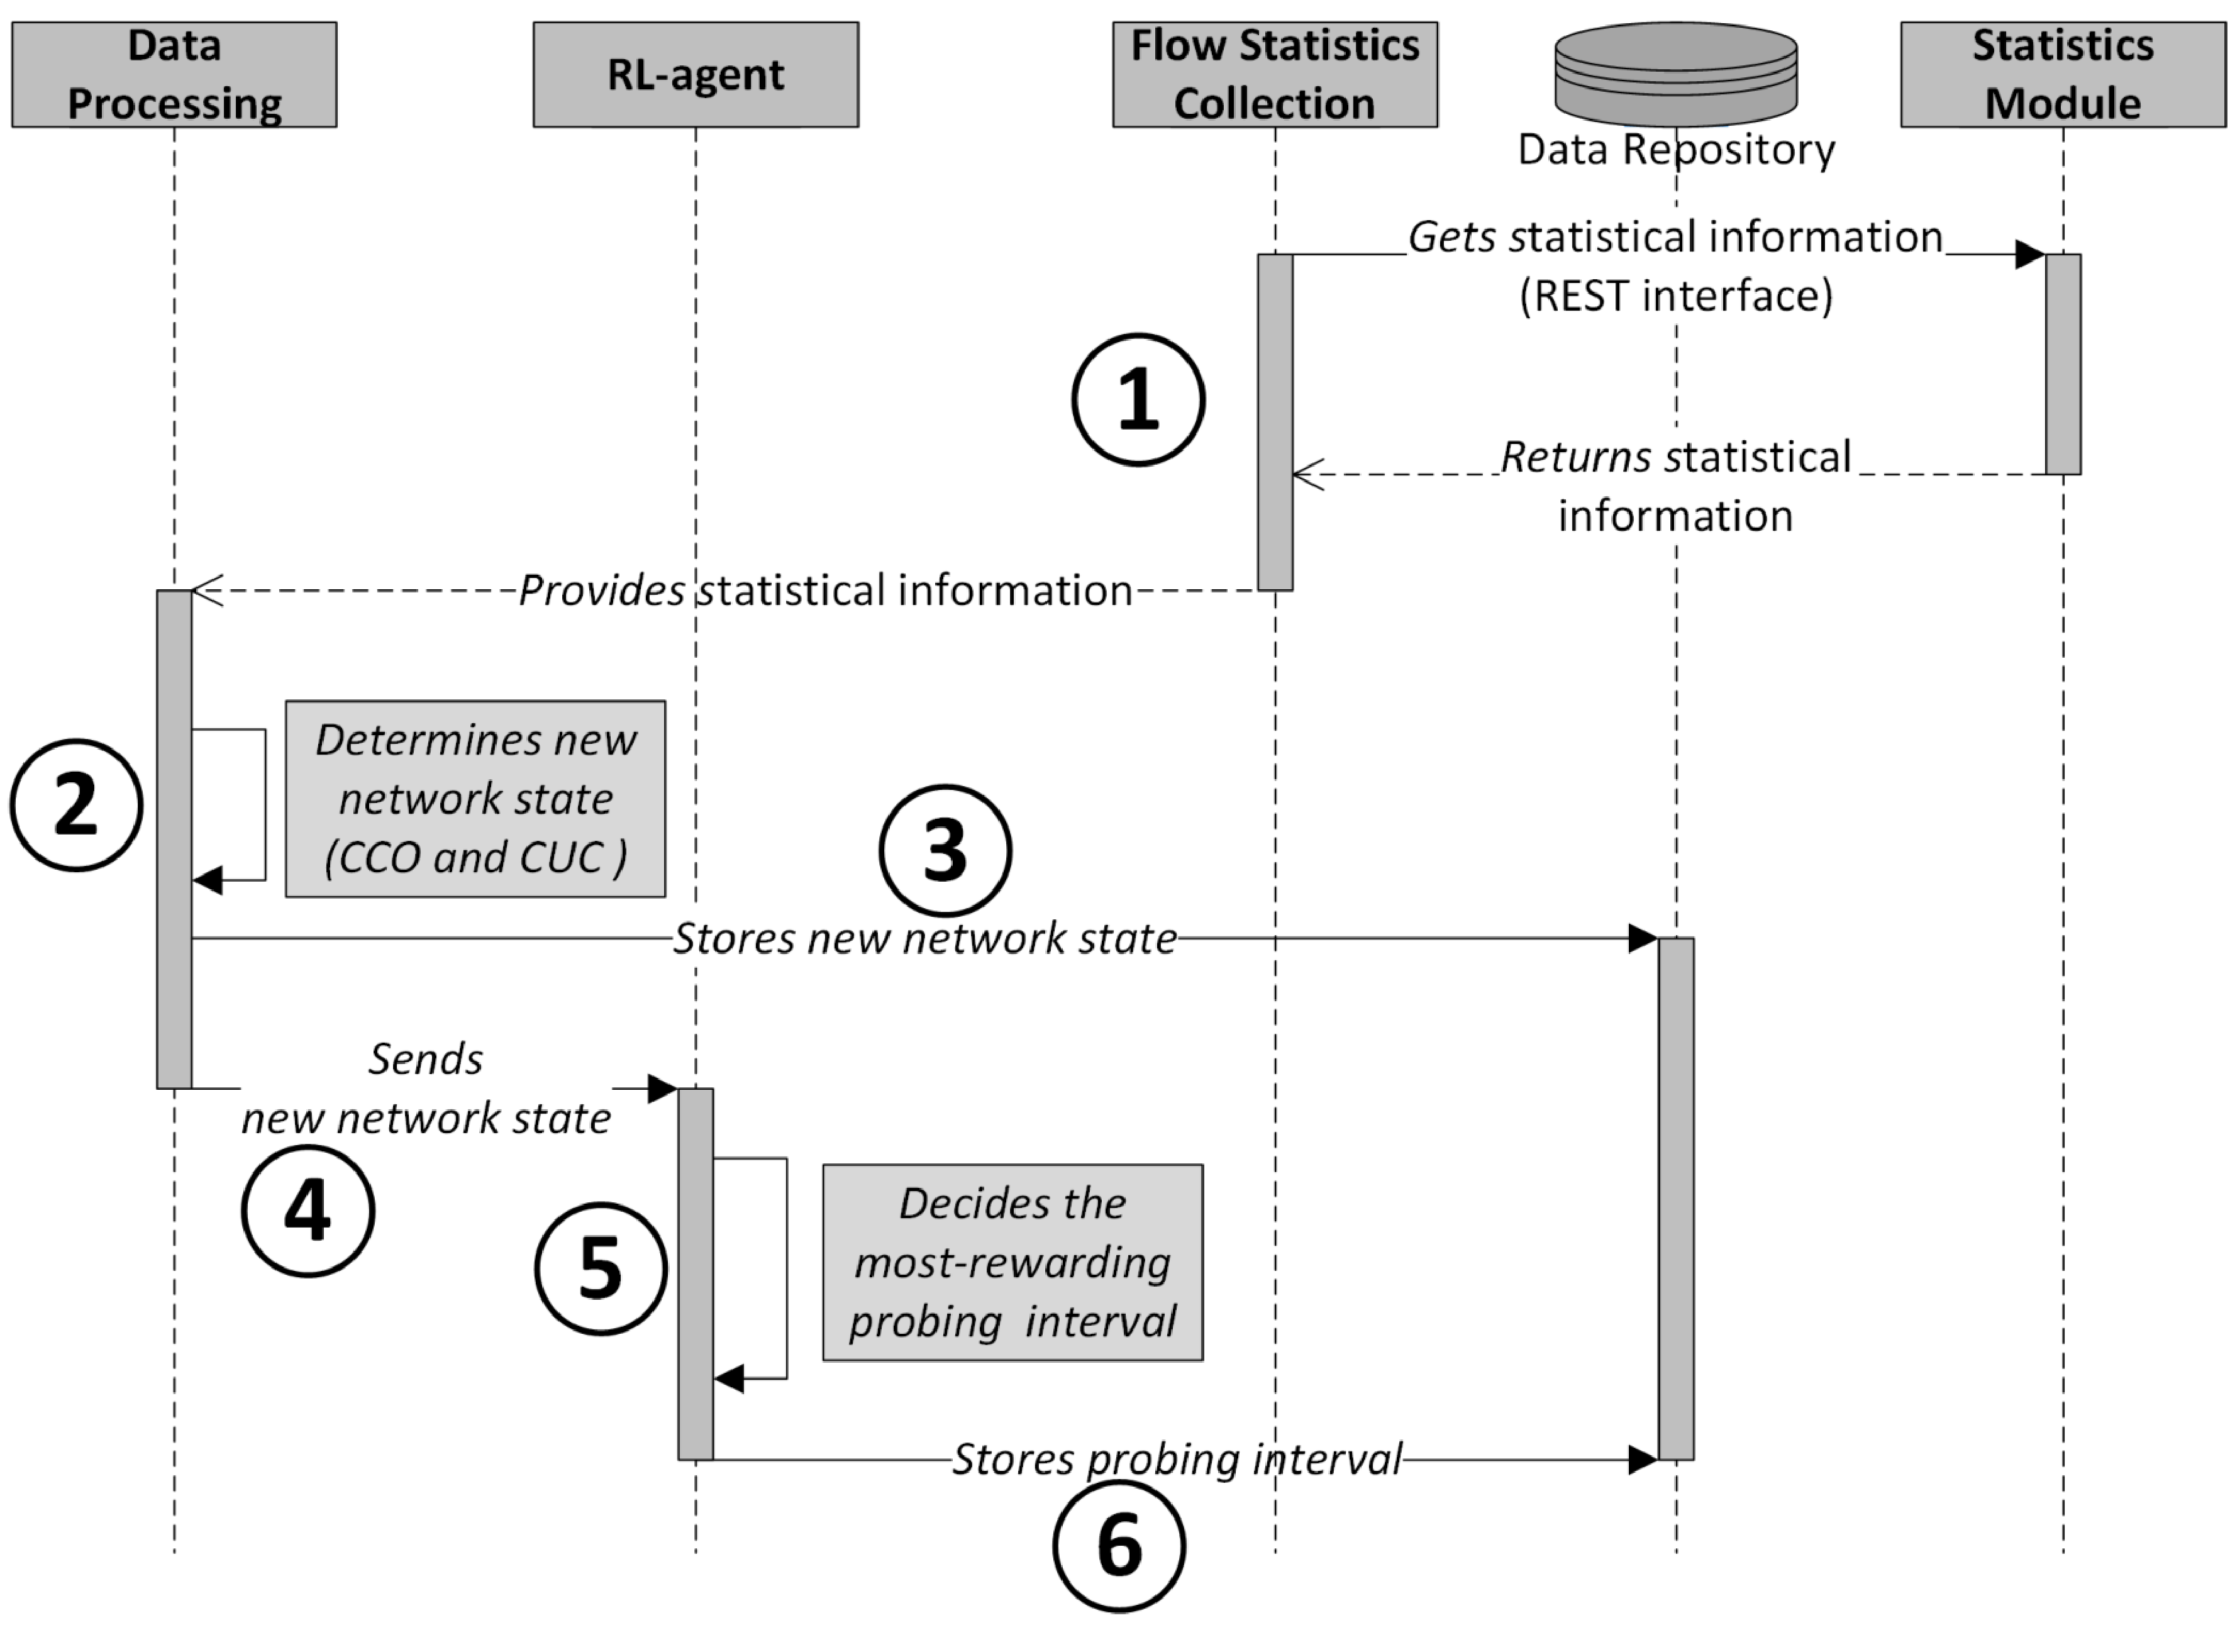
\includegraphics[width=0.90\columnwidth]{figures/Figure6-IPro-Sequence-diagram-mp}
    \caption{Sequence diagram of probing interval optimization process}
    \label{fig:sequence-diagram-mp}
\end{figure}

Figure~\ref{fig:sequence-diagram-mp} depicts how the elements of MP and KP interact in the probing interval optimization process.

\begin{enumerate}[label=\protect\circled{\arabic*}]
    \item Flow Statistics Collection extracts the statistical information from the Statistics Module located at CP and provides this information to Data Processing.
    \item Data Processing processes and organizes the information retrieved by Flow Statistics Collection to determine and such a new state by analyzing CCO and CUC.
    \item Data Processing stores the new state.
    \item Data Processing sends the new state to RL-agent located at KP.
    \item The RL-agent takes such a state to calculate the reward. Based on the reward, the RL-agent decides the most-rewarding probing interval intended to minimize CCO and CUC.
    \item The RL-agent stores this new probing interval to Data Repository. Probing Manager applies this interval that affects the network behavior again (\textit{i.e.}, initiates Statistics Collection Process). This process continues until the network administrator decides to stop IPro.
\end{enumerate}

\section{Final Remarks}
\label{sec:final_remarks_kap3}

Initially, in this chapter, the fundamental concepts about KDN and RL (in particular Q-learning)  were described. This master dissertation considered these concepts for proposing a KDN-based architecture (IPro) that keeps CCO and CUC within predefined thresholds and maintains an acceptable MA. Subsequently, the IPro architecture and its architectural elements were introduced and detailed. Finally, the RL-based algorithm (its functioning, computational complexity, and interactions) that determines the probing interval considering network traffic variations, CCO, and CUC was presented. 

\newpage{\null\newpage}
\newpage
\chapter{Evaluation}
\label{chapter:evaluation}
This chapter provides an extensive evaluation of the feasibility of using IPro as a practical approach (\textit{i.e.}, in terms of CCO, CUC, and MA) for intelligent probing in SDN. This chapter starts showing the test environment, including the SDN to monitor. After, this chapter presents the  IPro prototype developed and its impact (\textit{i.e.,} the change over the time of Probing Interval) in CCO, CUC, and MA (of the throughput) in the test environment. This chapter finishes showing the comparison of IPro with PPA and other adaptive approaches by quantitative and qualitative analysis, respectively.
\section{Setup}
\label{sec:setup}

\subsection{Test Environment}
\label{subsec:test_enviroment}

Figure~\ref{fig:campus_topo} presents the test environment used to evaluate IPro. This environment includes the campus network topology of the Federal University of Rio Grande do Sul \cite{isolani_2015:interactive}, the Ryu Controller, and the IPro prototype (\textit{cf.} Section ~\ref{subsec:prototype}). The monitored topology includes $11$ OpenFlow switches (version 1.3) that connect $230$ hosts from 7 laboratories (with 20, 30, and 40 hosts) and 4 administration offices (each one with 10 hosts) through links with a bandwidth of 10 Mbps each one. Furthermore, such topology includes a Web Server and a File Server connected in one of the administration offices. Each switch of the network is connected via a dedicated TCP channel to a remote Ryu controller used to coordinate network-wide forwarding decisions. The Mininet emulator \cite{lantz_2010:mininet} was used to deploy the monitored topology, which runs on a Ubuntu server with an Intel i7-4770 2.26 GHz and 8GB RAM. The Ryu Controller runs on a Ubuntu server with a Core i7-4770 processor and 2GB RAM.

\begin{figure}[H]
    \centering
    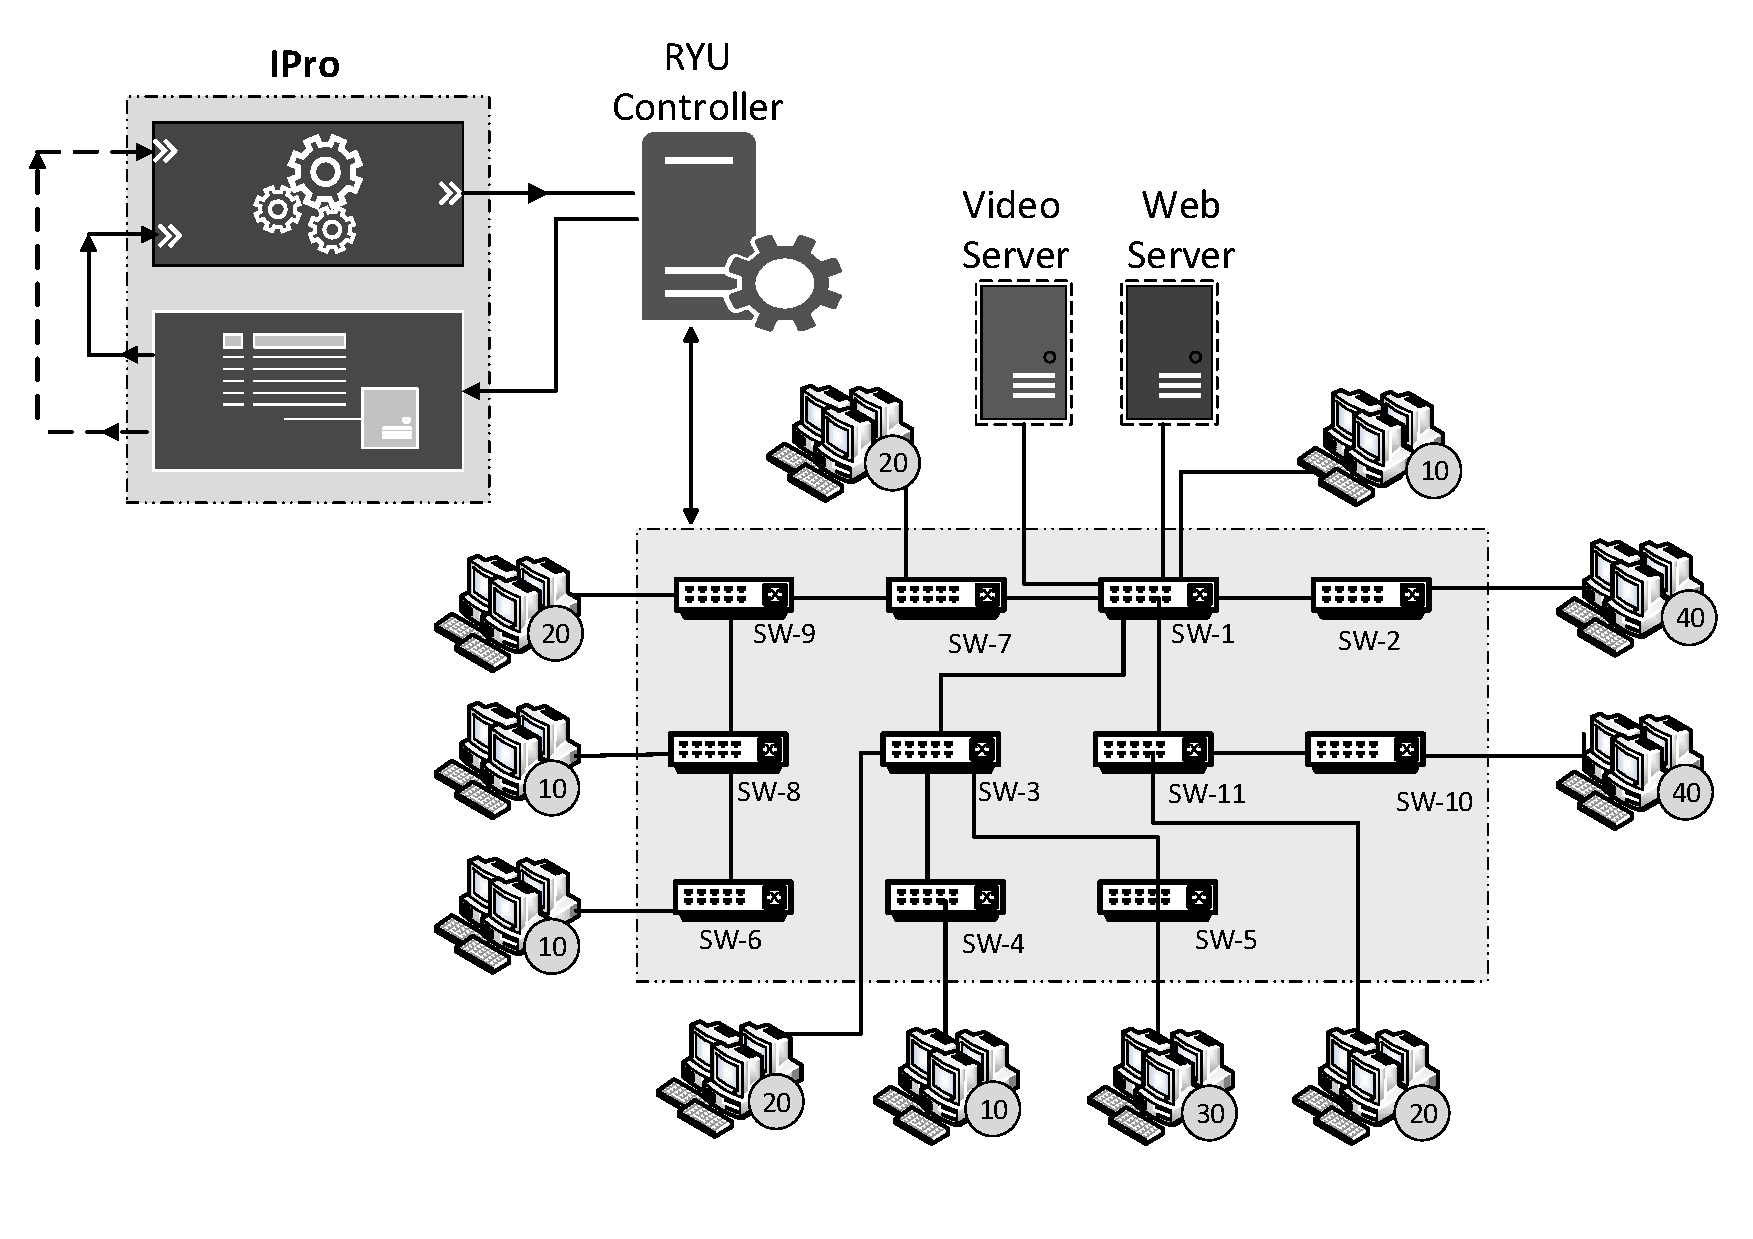
\includegraphics[width=0.75\columnwidth]{figures/Fig4-topology}
    \caption{Test Environment}
    \label{fig:campus_topo}
\end{figure}

To reliably test IPro, a realistic evaluation framework reflecting current and forecasted traffic patterns (\textit{e.g.,} web, P2P, and video) was used. In this master dissertation, to two measurement studies that investigate the composition of realistic traffic patterns \cite{labovitz_2011:interdomain, maier_2009:dominant} was resorted. The results indicate the dominance of Web traffic, amounting to 52\% overall measured traffic, followed by video traffic with 25-40\% of all traffic, while P2P traffic constituting only 18.3\% of total traffic. Thus, in all experiments, only Video and Web traffic was generated, in a proportion of 75\% to 25\%, respectively.\\

The Video traffic was generated by using the VLC media player \cite{Muller:2011:VMP:2072298.2072429} that can be used as a server and as a client to stream and receive video streams. The Web traffic was generated by using the Apache Server \cite{Mockus:2000:CSO:337180.337209} and http-clients based on Linux wget. These servers and clients were included in the campus topology. In this evaluation was assumed that all 230 hosts are active during the whole experiment time and place a request on average every 30 seconds. Furthermore, all experiment results have a confidence level equal to or higher than 95\%.
\subsection{Prototype}
\label{subsec:prototype}

Figure~\ref{fig:prototype_ipro} depicts the IPro prototype including: \textit{RL-agent}, \textit{Data Processing}, \textit{Flow Statistics Collection}, \textit{Data Repository}, \textit{Probing Manager}, \textit{Query Manager}, and \textit{Statistics Module}. \textit{RL-agent} and \textit{Data Processing} were developed and deployed using version 1.15 of Numpy that is the fundamental Python package for scientific computing. \textit{Probing Manager}, \textit{Query Manager}, and \textit{Statistics Module} were developed using the REST-based API provided by Ryu. This API helps to retrieve the switch statistics. \textit{Flow Statistics Collection} was developed using the Ryu API based on Python. \textit{Data Repository} was developed in MySQL. The IPRo prototype (including all test scripts) is available in \cite{castillo:ipro}.

\begin{figure}[H]
    \centering
    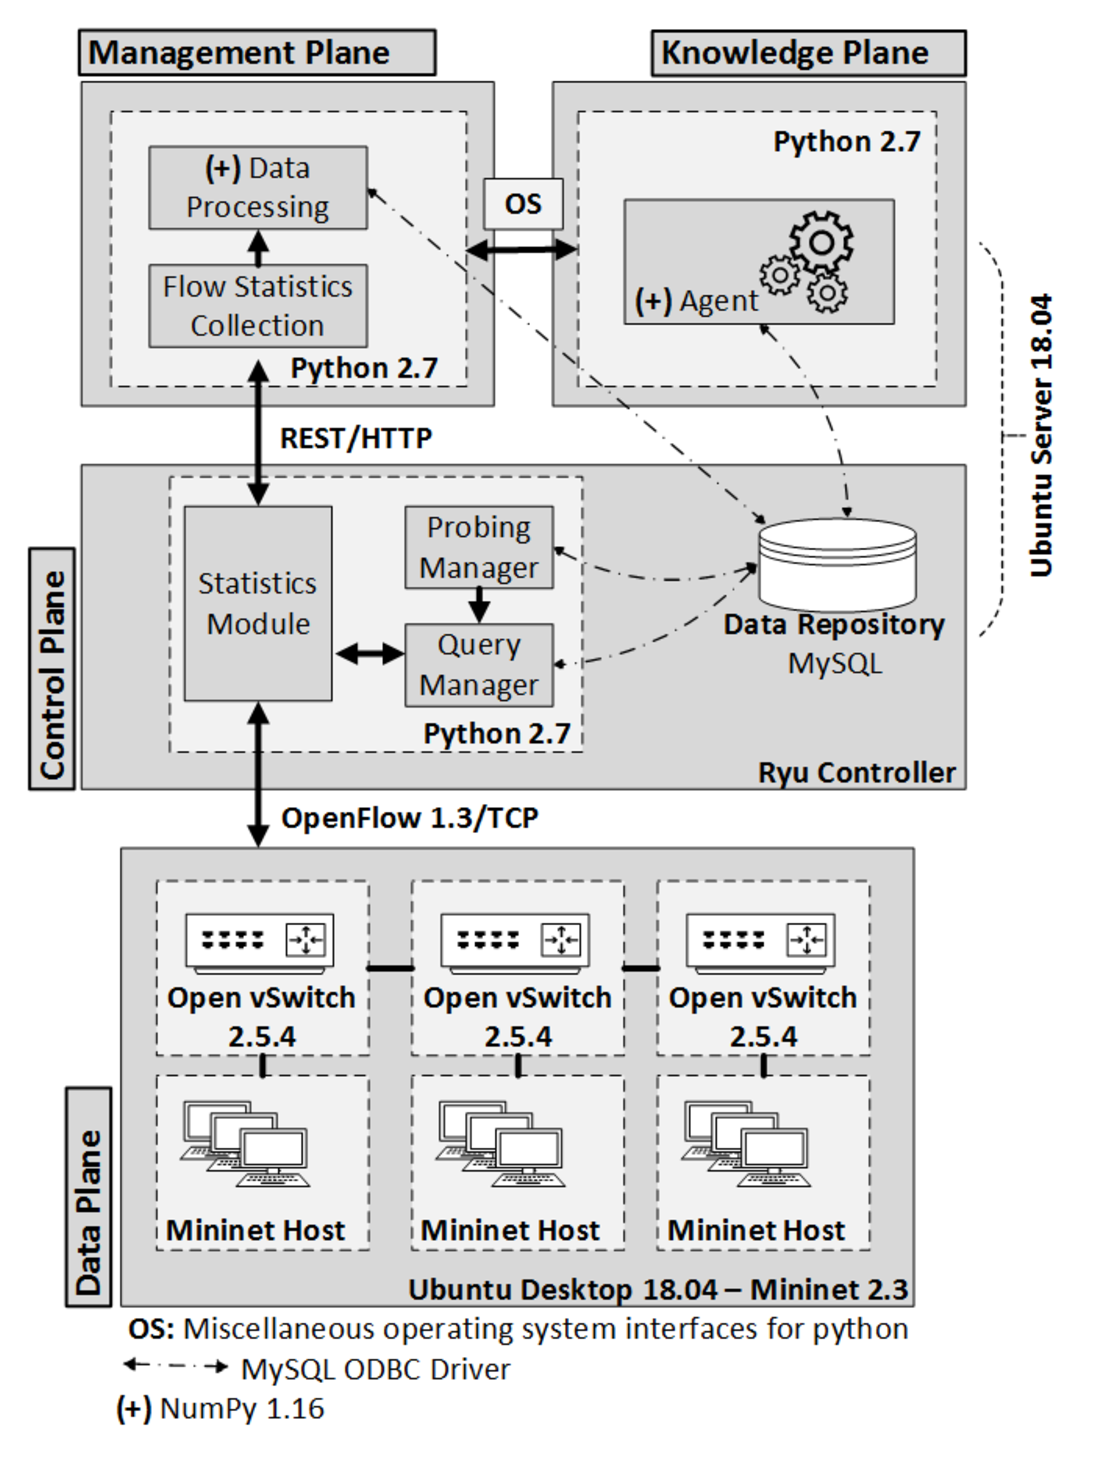
\includegraphics[scale=0.5]{figures/Fig5-IPro-prototype}
    \caption{IPro - Prototype}
    \label{fig:prototype_ipro}
\end{figure}

It is important to highlight that the \textit{Statistics Module} interacts with DP by the OpenFlow Protocol \cite{onf_2012:openflow}. This protocol was used because it has progressively turned on the SBI \textit{de-facto} standard in SDN \cite{nunes_2014:survey_past_present_future}. OpenFlow describes an open protocol that allows software applications to program (\textit{i.e.}, add, update, and delete flow entries) the flow table of the OpenFlow-compliant switches. In particular, the \textit{Statistics Module} uses the OpenFlow version 1.3. Specifically, this module uses two Read-State (Request-Reply) messages to collect information from the switch, such as current configuration, statistics, and capabilities. The controller sends a Read-State Request message to the switches to request the traffic statistics of flows. The switches communicate to the controller the requested traffic statistics via Read-State Reply messages. To get OpenFlow details,  the reader to Openflow specification is refered \cite{onf_2012:openflow}.

\subsection{Space of States}
\label{subsec:space_states}

To determine the finite space of states (\textit{cf}. Equation~\ref{equ:states_model}) that the IPro RL-agent needs to operate, first, the CCO (\textit{cf}. Equation~\ref{equ:load}), CUC (\textit{cf}. Equation~\ref{equ:load_cpu}), and MA (\textit{cf}. Equation~\ref{equ:ma}) were estimated and experimentally measured when the probing interval varies. The probing intervals between 1 and 15 seconds were manually tested (in steps of 1 second). For each interval, the test duration was 600 seconds. Second, the CCO and CUC were discretized by using the obtained results.

\subsubsection{Control Channel Overhead}
Aiming at determining the space of states that the IPro RL-agent needs to operate, Figure~\ref{fig:control_channel_load_behavior} presents the impact of the probing intervals on CCO. If the network is monitored with a probing interval upper or equal than 5 seconds, the overhead is lower than 12\%. When this interval is smaller than 5 seconds the overhead increases (top than 20\%) due to the big size and quantity of Read-State (Request-Reply) messages (\textit{cf}. Equation~\ref{equ:load}). These results corroborate that the probing interval affects CCO significantly.

\begin{figure}[h!]
    \centering
    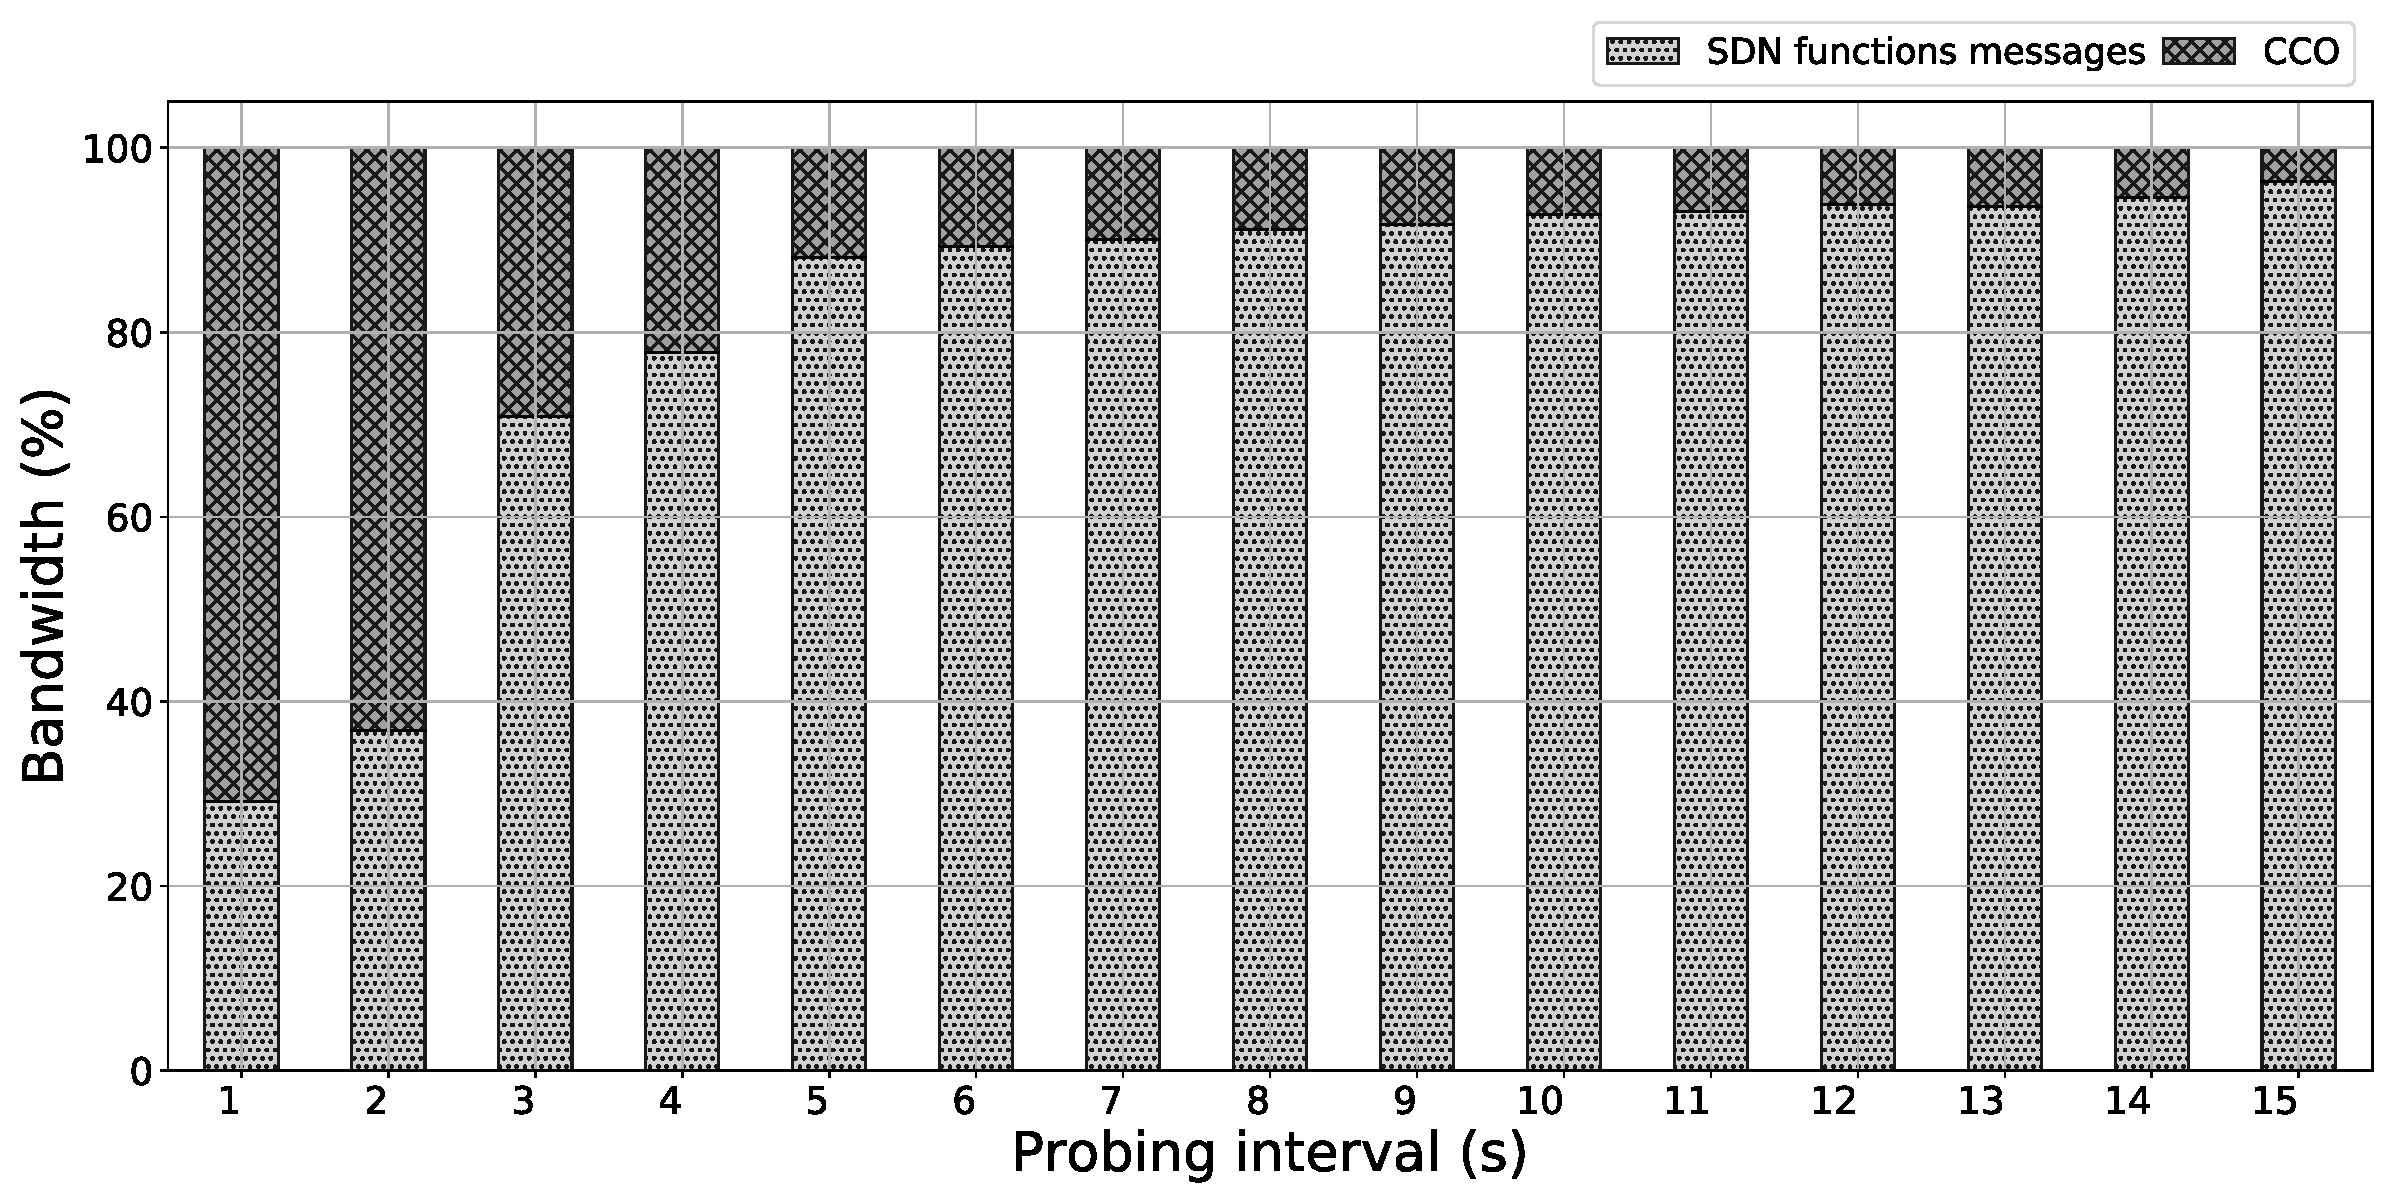
\includegraphics[width=1.0\textwidth]{figures/Fig7-control-channel-behavior}
    \caption{CCO Variation}
    \label{fig:control_channel_load_behavior}
\end{figure}

\subsubsection{CPU Usage of the Controller}
Aiming at determining the space of states that the IPro RL-agent needs to operate, Figure~\ref{fig:cpu_behavior} presents the impact of the probing intervals on CUC. If the network is monitored with a probing interval upper or equal than 5 seconds, CUC increases on average 8.5\% approximately. Nevertheless, when this interval is smaller than 5 seconds, CUC increases (top than 20.5\%) because the controller collects statistics information more frequently. As a consequence, the controller CPU must process a higher amount of instructions per second for (de)fragmenting and reading the Read-State messages. Overall, these results corroborate that the probing interval can affect CUC significantly.

\begin{figure}[h!]
    \centering
    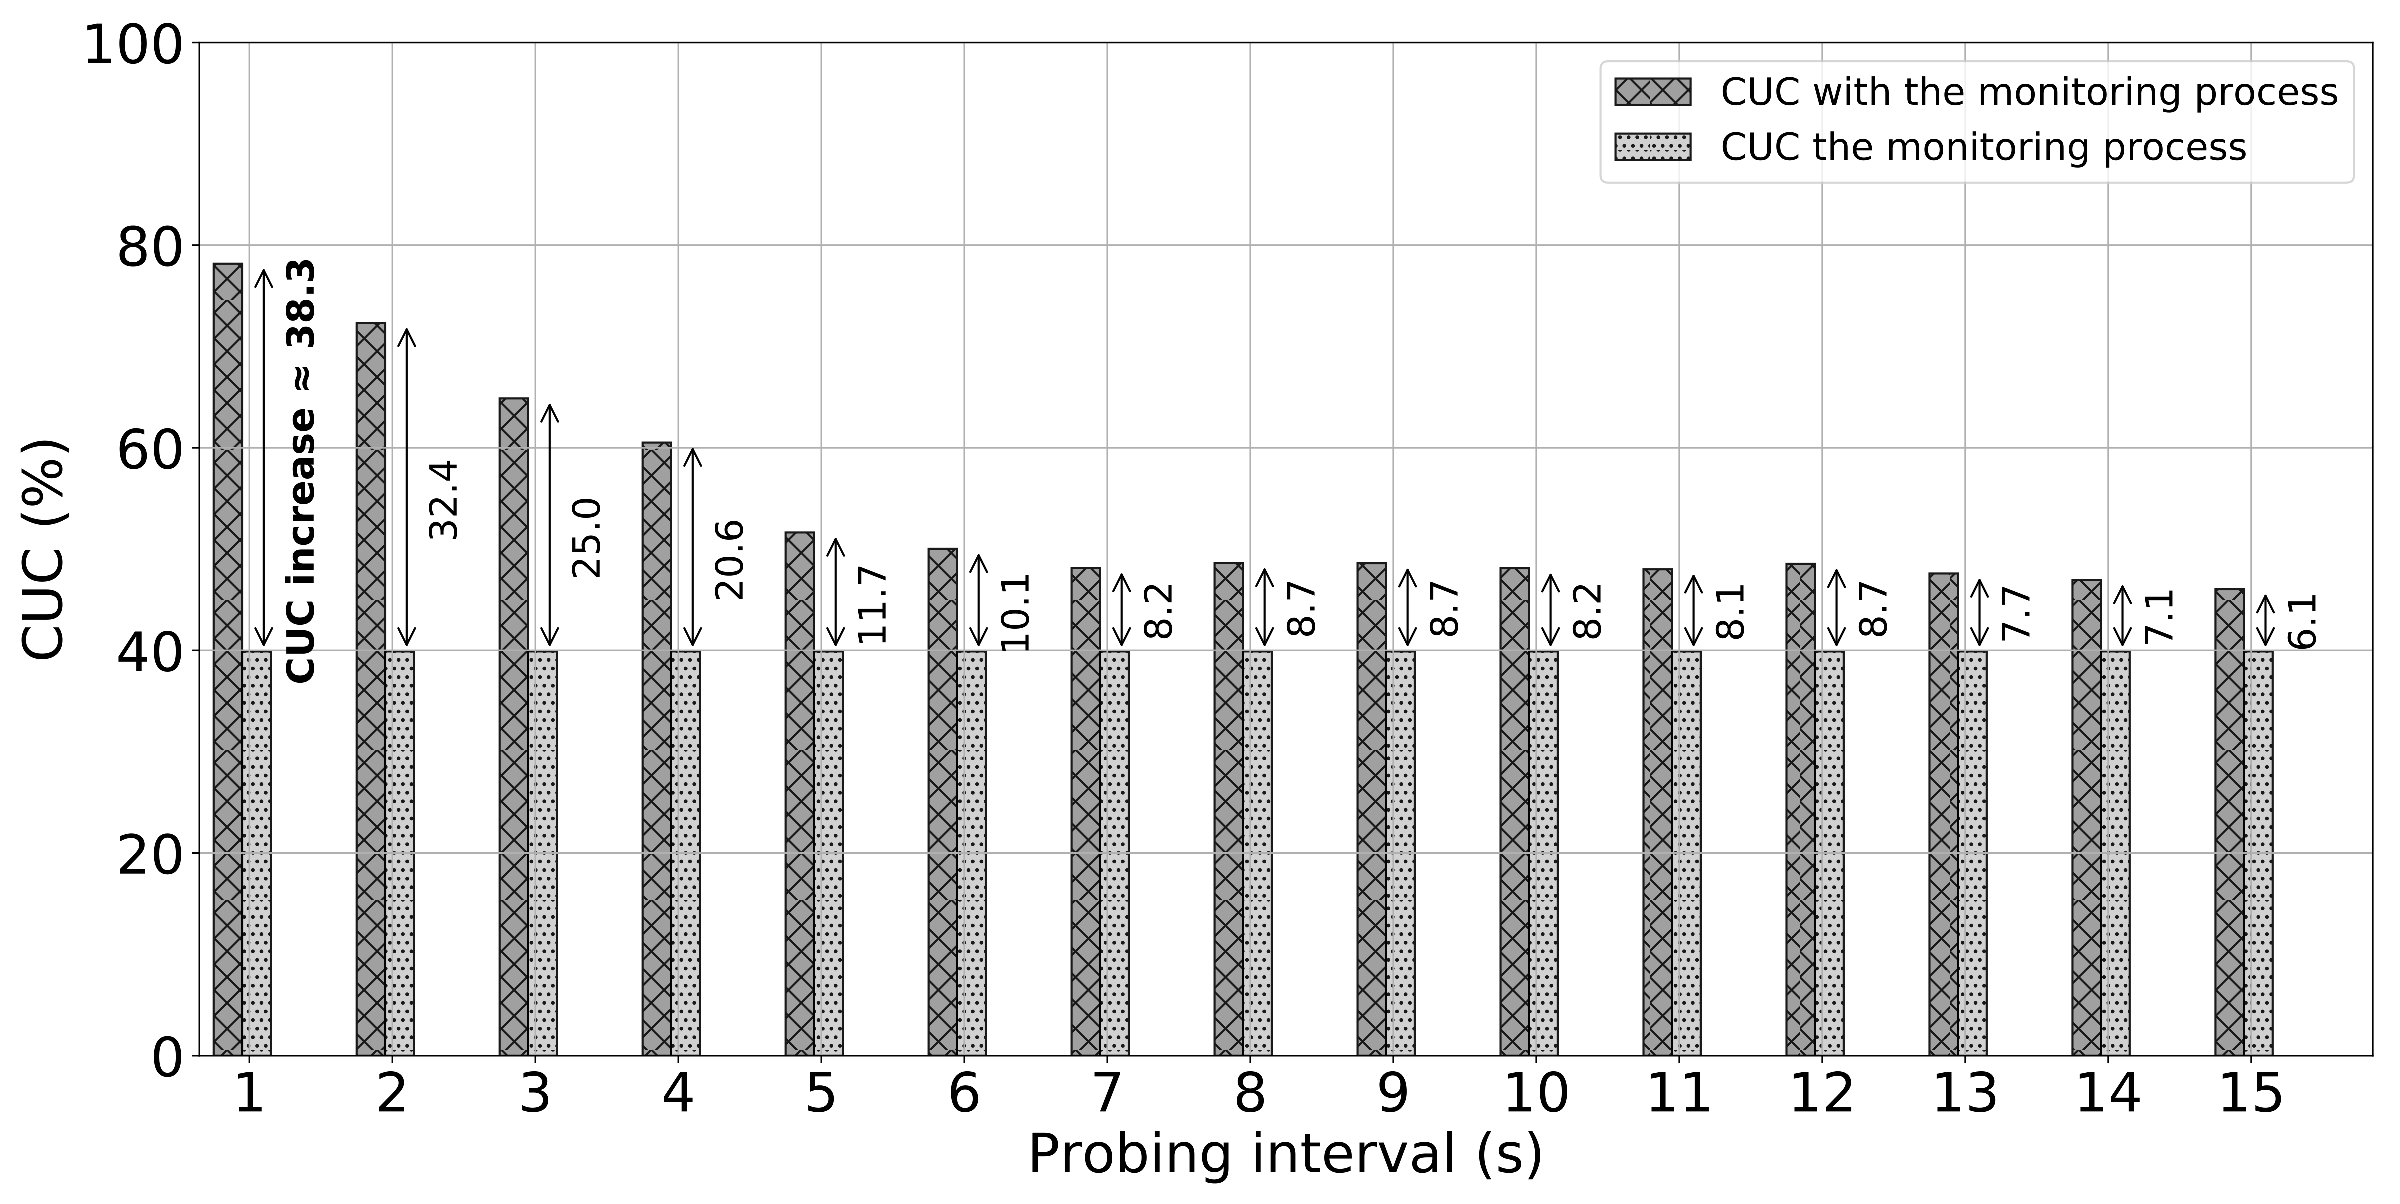
\includegraphics[width=1.0\columnwidth]{figures/Fig6-cpu-usage}
    \caption{CUC Variation}
    \label{fig:cpu_behavior}
\end{figure}

\subsubsection{Monitoring Accuracy}

\begin{figure}[h!]
    \centering
    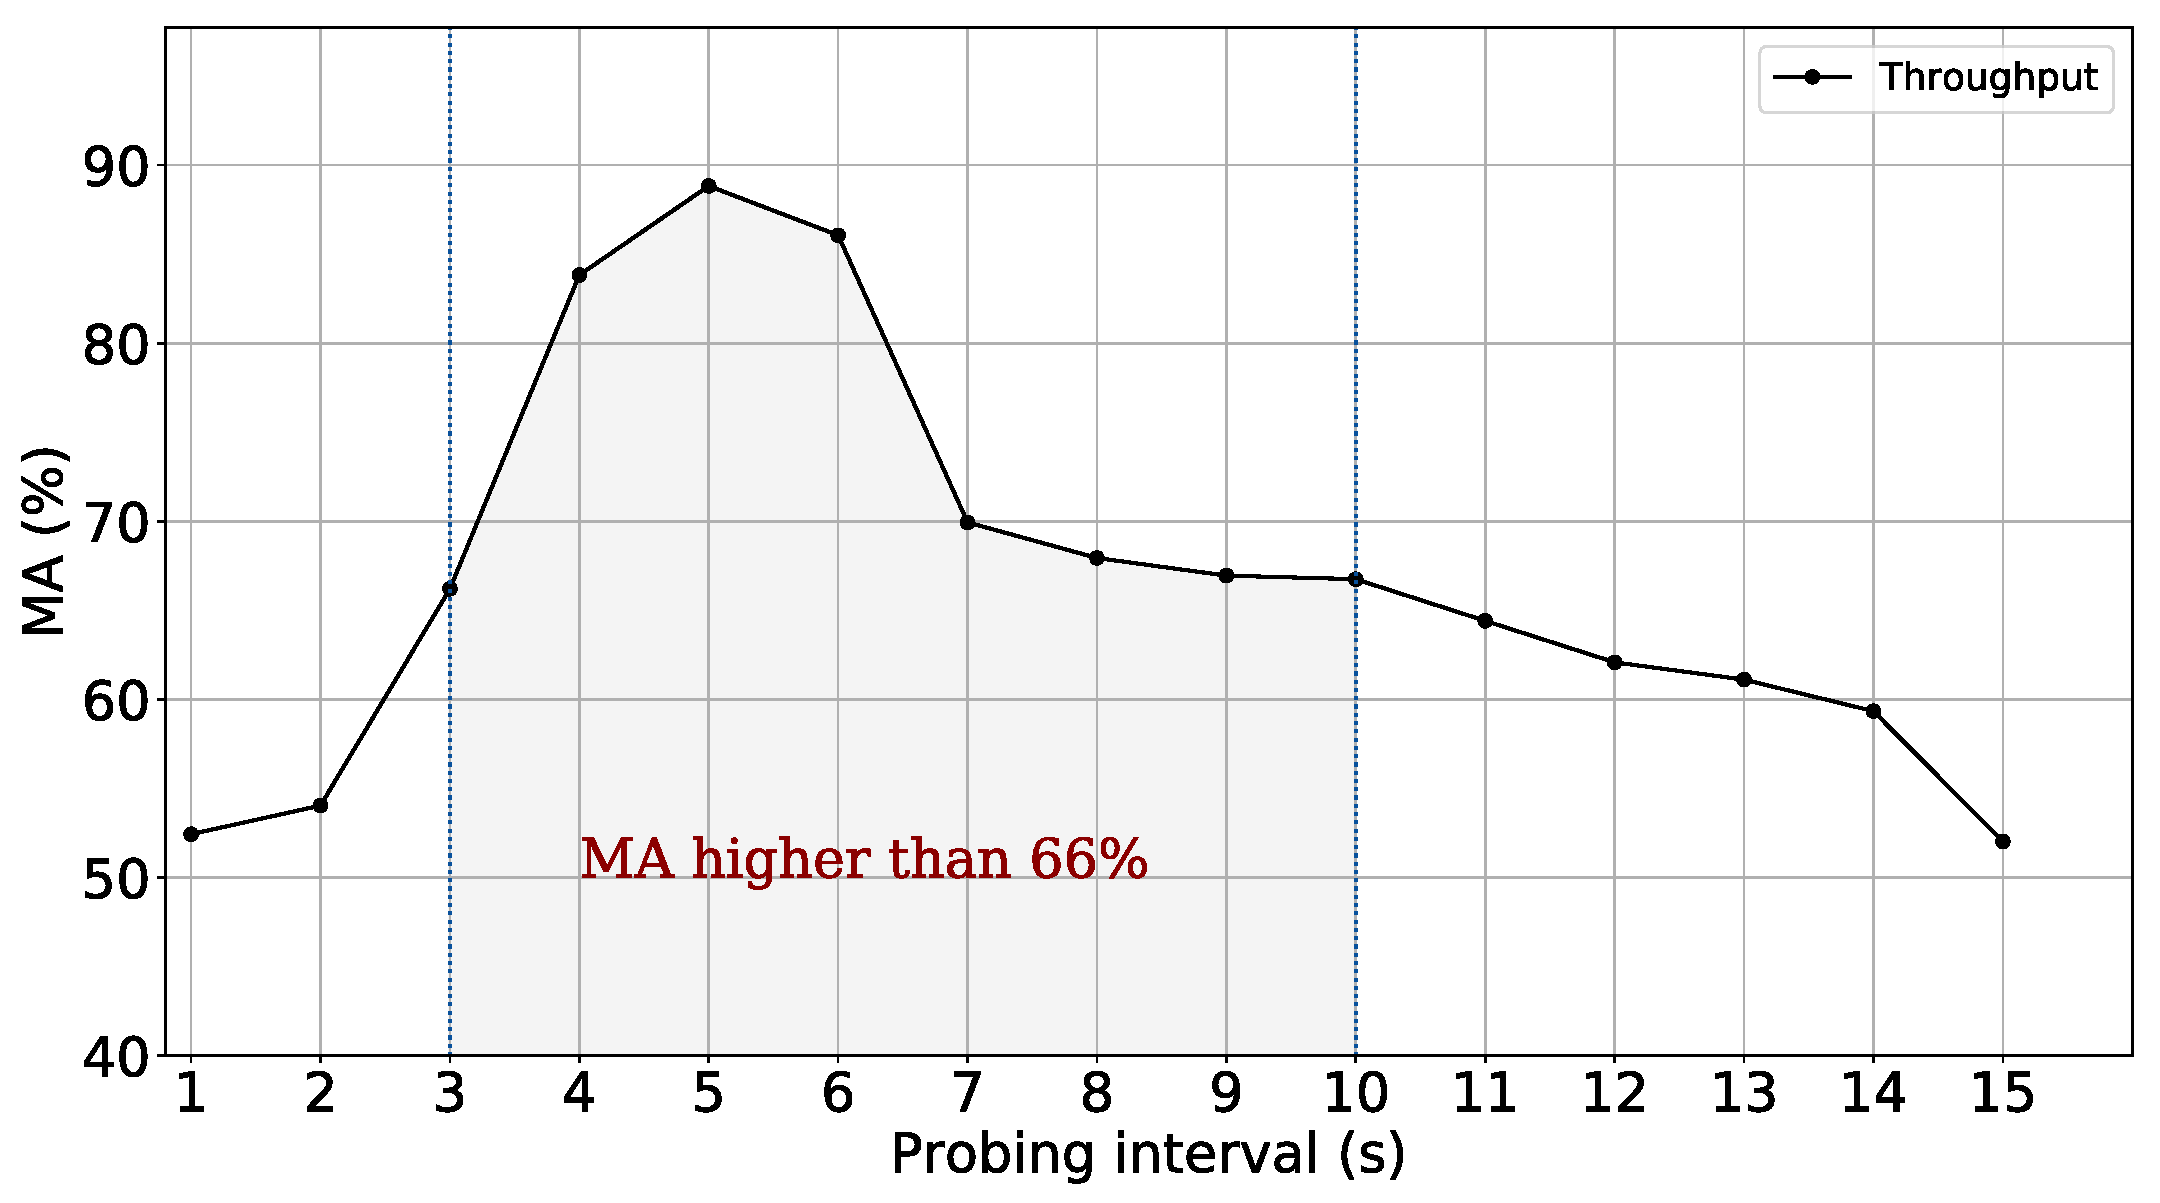
\includegraphics[width=1.0\columnwidth]{figures/Fig9-throughput}
    \caption{MA of throughput }
    \label{fig:throughput}
\end{figure}

To evaluate MA, the throughput metric was measured in each probing interval and determine its respective accuracy using Equation~\ref{equ:ma}. Figure~\ref{fig:throughput} depicts the evaluation results, disclosing that MA in the throughput measured is higher than 80\% when the probing interval varies between 4 and 6 seconds. In particular, the interval of 5 seconds reports the highest MA (88.83\%). In turn, the intervals of 6 seconds and 4 seconds achieve an MA equal to 86.06\% and 83.83\%, respectively. Nonetheless, MA reduces considerably for the other probing intervals. For instance, the interval of 7 seconds accomplishes an MA lower than 69.93\% due to the reduction in the quantity of collected information. In turn, the probing intervals 1, 2, and 3 seconds lead to high CCO that interferes with SDN management messages. Furthermore, these intervals also lead to high CUC that compromises the correct operation of the controller and, so, of the underlying data plane. These two facts deteriorate the correct operation of the network generating high TCP errors and low processing of SDN management messages (\textit{cf}. Figure~\ref{fig:tcp-erros}). Therefore, the MA of data collected is also affected. In summary, the above results corroborate that the probing interval affects MA significantly.

\begin{figure}[h!]
    \centering
    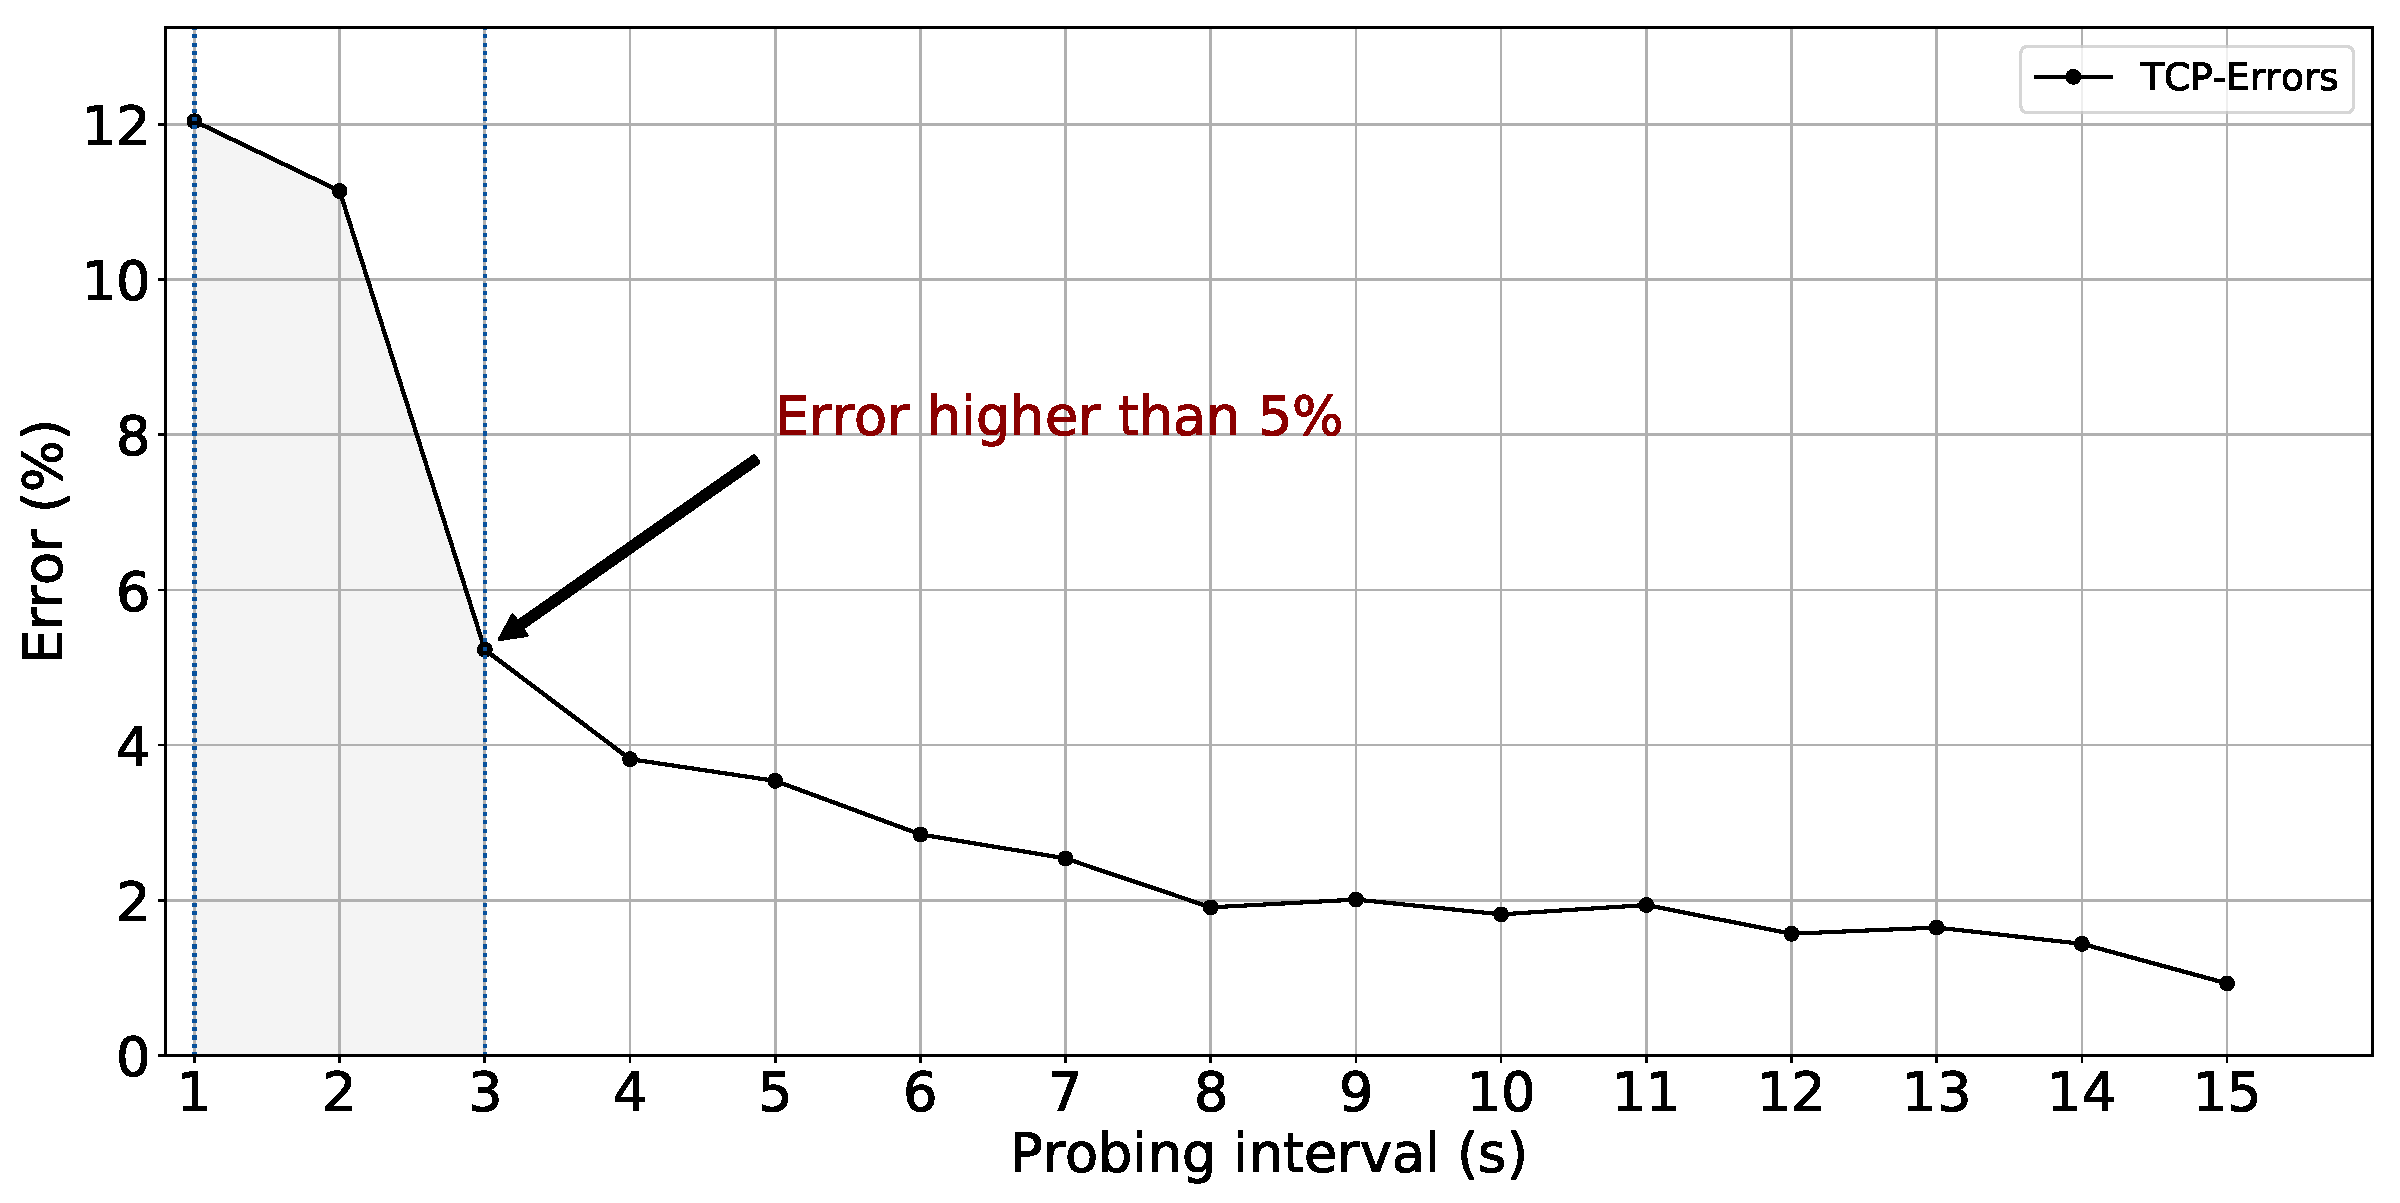
\includegraphics[width=1.0\textwidth]{figures/Figure9b-tcp-errors}
    \caption{TCP errors generated by Monitoring Interference}
    \label{fig:tcp-erros}
\end{figure}

\subsubsection{Spaces Discretization}
Since IPro is RL-based, it models its environment as a finite MDP. In order to get a finite space of states, the CCO and CUC were discretized by using the results above presented (\textit{cf.} Figures~\ref{fig:control_channel_load_behavior} and ~\ref{fig:cpu_behavior}) as follows:

\begin{enumerate}
    \item The values of CCO and CUC are represented in the interval $\left [ 0,1 \right ]$, where 0 represents 0\% and 1 represents 100\%.
    \item The policy 1 (related to the threshold $\omega$) is set to 80\% aiming at preventing response times of controller upper than 1 millisecond \cite{repas_2015:performance_cpu}. Thus, \\
    CCO: $ l =\left \{ \left [ 0,0.4 \right ), \left [ 0.4,0.5 \right ), \left [ 0.5,0.6 \right ), \left [ 0.6,0.7 \right ) ,\left [ 0.7,0.8 \right )\right \}$.
    \item The policy 2 (related to the threshold $\chi$) is set to 80\% targeting to avoid interference with essential SDN functions (\textit{e.g.}, packet forwarding and route updating) and the reduction of network performance \cite{xu_2017:wildcard_requests}. Thus, \\
    CUC: $cpu=\left \{ \left [ 0,0.4 \right ),\left [ 0.4,0.5 \right ),\left [ 0.5,0.6 \right ),\left [ 0.6,0.7 \right ),\left [ 0.7,0.8 \right ) \right \}$.
    \item The Probing Interval: $i = \left \{\left [ 4,10 \right ] \right \}$. 
\end{enumerate}

It is important to highlight that CCO and CUC can be divided into smaller sub-intervals to facilitate the RL-agent decision making process. However, smaller intervals increase the size of the space of states and, so, slow down the learning process convergence rate. Thus, the discretized space of states is:

{\setlength{\mathindent}{3cm}
\begin{equation}
    \begin{split}
      S\equiv f\left ( i, l, cpu \right ): & i\in \left [ 4,10 \right ], l=\left \{ 0,0.4,0.5,0.6,0.7,0.8 \right \},\\ 
      & cpu=\left \{ 0,0.4,0.5,0.6,0.7,0.8 \right \} 
    \end{split}
    \label{equ:states}
\end{equation}
}
\section{Intelligent Probing Behavior}
\label{sec:ipro_behavior}

To evaluate the IPro prototype (\textit{cf}. Algorithm 3), its impact (\textit{i.e.,} the change over the time of Probing Interval) in CCO, CUC, and MA (of the throughput) was tested in the test environment described in Section~\ref{sec:setup}. Figure~\ref{fig:load_behavior} depicts the evaluation results, disclosing diverse facts.

%\begin{figure}[htb]
\begin{figure}[h!]
\centering
        \begin{minipage}[t]{1.0\textwidth}
            \centering
            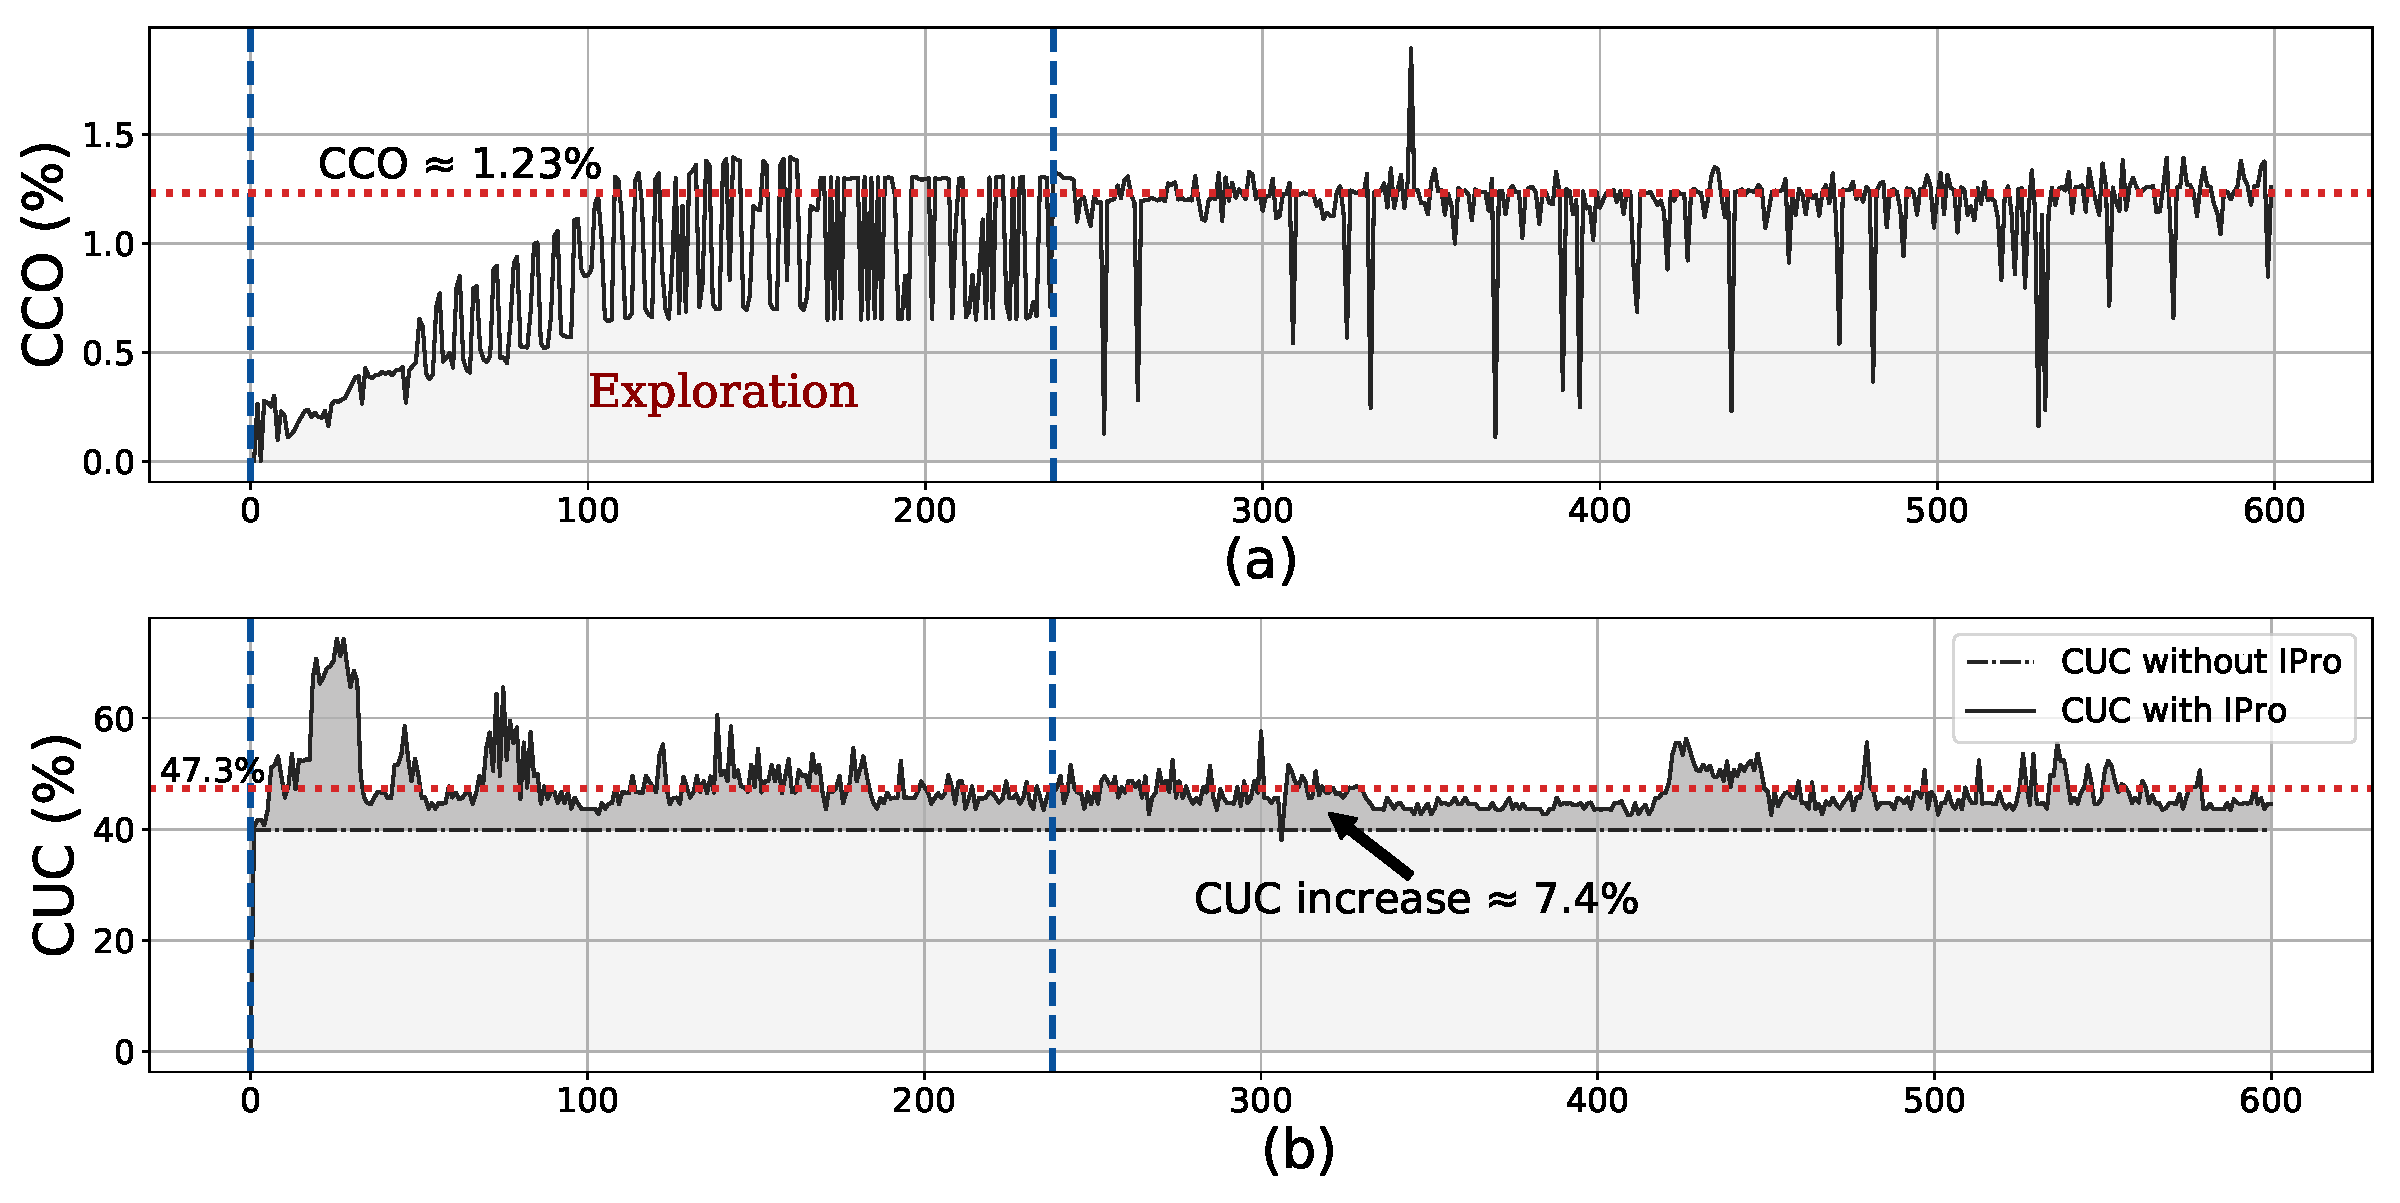
\includegraphics[width=\textwidth]{figures/Figure12a-IPro-behavior-MA-CCO-CUC}
            %\subcaption{Image 1.}\label{fig:1}
        \end{minipage}
        \hfill
        \begin{minipage}[t]{1.0\textwidth}
            \centering
            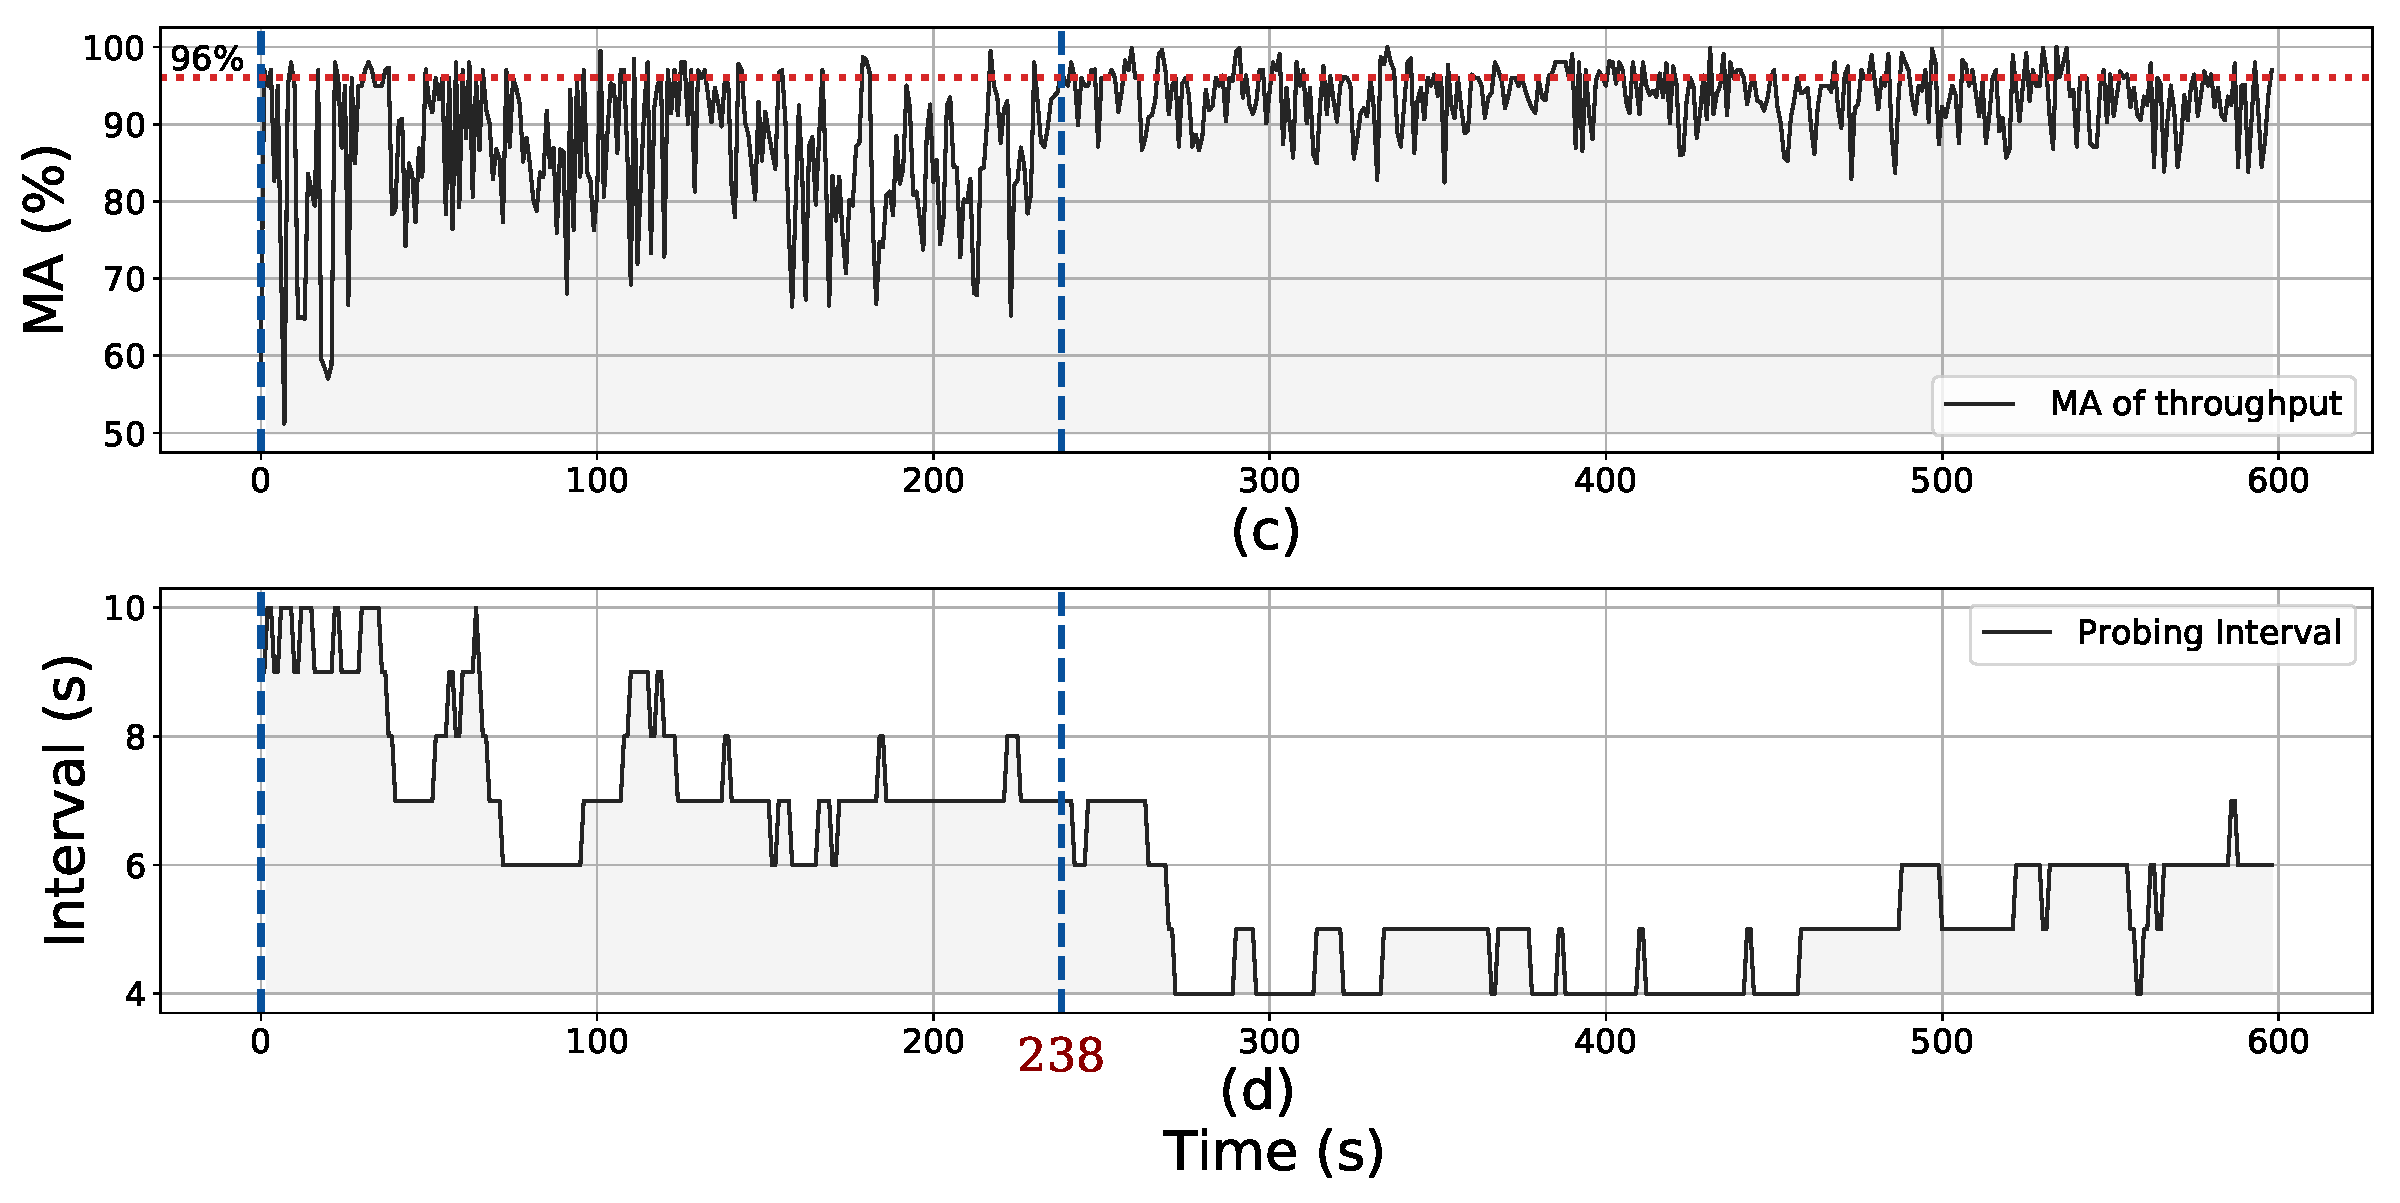
\includegraphics[width=\textwidth]{figures/Figure12b-IPro-behavior-MA-CCO-CUC}
            %\subcaption{Image 2.}\label{fig:2}
        \end{minipage}
        \vspace{-0.5cm}
        \caption{Behavior of the CCO, CUC, MA, and Probing Interval}
        \label{fig:load_behavior}
\end{figure}

\begin{itemize}
    \item During the first 238 seconds (convergence time), CCO, CUC, and MA present a highly fluctuating behaviour Figure~\ref{fig:load_behavior}(a,b,c). This behaviour is because the RL-agent does not have a previous knowledge (\textit{i.e.}, the Q-function starts empty and is filled during this time). Therefore, it is necessary that such an agent starts the exploration process to determine the effect of each action on the network status (\textit{i.e.}, learning process). Figure~\ref{fig:load_behavior}(d) illustrates how the Probing Interval changes during the learning process. As the learning process advances, the RL-agent visits each state of the space of states (\textit{cf.} Equation~\ref{equ:states}) multiple times aiming at finding the most-rewarding probing strategy (\textit{i.e.}, the convergence of the learning process).
    \item After the convergence time, IPro has a CCO near to 1.23\%, a CUC around 7.4\%, and a MA about 96\%. This result demonstrates that, in terms of CCO, CUC, and MA, IPro has good behavior. When the learning process tends to converge, the fluctuations of CCO, CUC, and MA decrease to a smaller radius. This convergence is because a normal distribution function (\textit{cf}. Equation~\ref{equ:reward}) was chosen whereby IPro gradually moves to adjacent states to the target state (\textit{i.e.}, calibrates the action-value function). In particular, IPro provides the best behaviour regarding CCO, CUC, and MA when it probes the network with intervals between 4 and 6 seconds.
    \item It is important to highlight that IPro does not stop its learning because, in real networks, the environment will always be changing and evolving.
\end{itemize}

To determine the performance of IPro itself, the consumption of CPU and memory of its RL-agent was evaluated. Figure~\ref{fig:rl-agent_behavior} depicts the evaluation results, disclosing that this RL-agent does not consume intensively the KP resources, approximately 1\% -2\% of CPU and 30MBytes. These results demonstrate that, in terms of CPU and memory, IPro RL-agent is efficient.

\begin{figure}[h!]
    \centering
    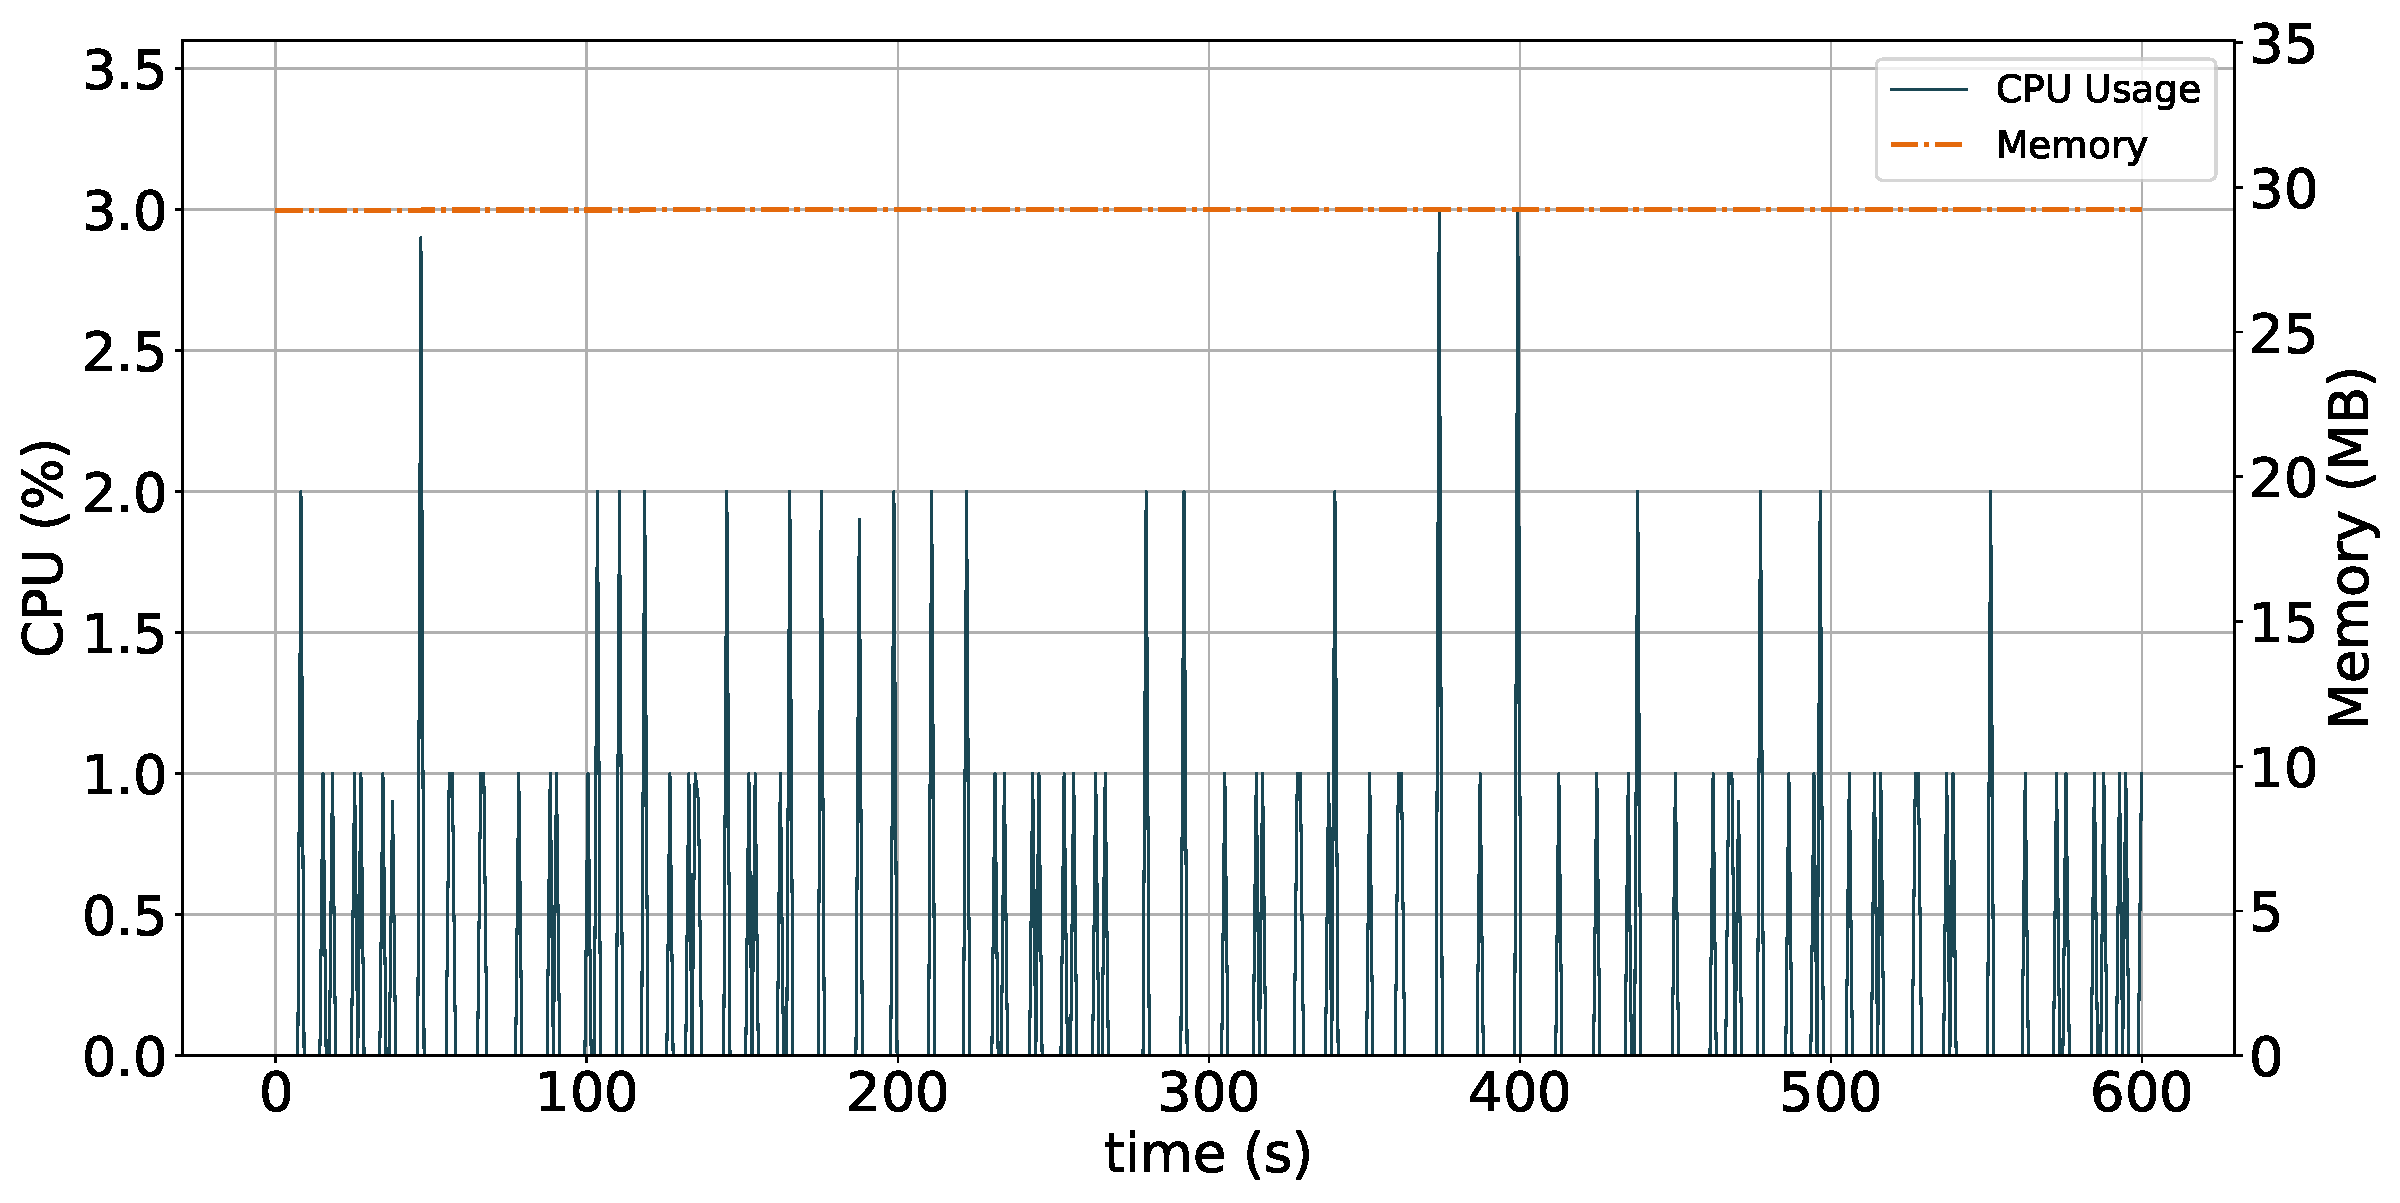
\includegraphics[width=1.0\textwidth]{figures/Figure13-cpu-usage-rl-agent}
    \caption{Behavior of the CPU usage and memory of RL-agent}
    \label{fig:rl-agent_behavior}
\end{figure}
\section{Comparison}
\label{sec:ipro_performance}
IPro was compared to PPA (\textit{i.e.,} a pull-based approach targeted to monitor the network switches with a pre-defined probing interval) regarding CCO, CUC, and MA after and before the convergence time. The probing intervals tested were ranging between 1 and 15 seconds (in steps of 1 second). For each interval, the test was performed 32 times during 600 seconds (the initial 238 seconds correspond to convergence time), aiming at obtaining the average of CCO, CUC, and MA. Next, only the 4, 5, and 6 seconds probing intervals was analyzed because, in them, the MA of measurements of both throughput and delay metrics is higher than 80\%. Finally, the comparison of IPro with other adaptive approaches was extended by a qualitative analysis.

\subsection{After Converging}
\label{converge}

\fontsize{7}{8}\selectfont
{\renewcommand{\arraystretch}{1.4}
\begin{table*}[!htp]
\scriptsize
\begin{center}
\footnotesize
\begin{tabularx}{\linewidth}{P{30mm}P{30mm}P{28mm}P{28mm}P{28mm}}
\hline
\textbf{\rotatebox[origin=c]{0}{Probing }}& \textbf{\rotatebox[origin=c]{0}{MA of}} &\textbf{\rotatebox[origin=c]{0}{MA of}}&\textbf{\rotatebox[origin=c]{0}{CUC [\%]}}&\textbf{\rotatebox[origin=c]{0}{CCO [\%]}}\\[-2ex]
\textbf{\rotatebox[origin=c]{0}{Interval [s] }}& \textbf{\rotatebox[origin=c]{0}{Throughput [\%]}} &\textbf{\rotatebox[origin=c]{0}{Delay [\%]}}&\textbf{\rotatebox[origin=c]{0}{}}&\textbf{\rotatebox[origin=c]{0}{}}\\\hline

\rowcolor{gray!20} IPro  &  96.17 & 94.78&  7.40 & 1.23  \\\hline
PPA with 4     &  83.59 &  82.50&   20.60 & 17.40  \\\hline
PPA with 5     &  91.38 &  89.50&   11.70 & 11.45  \\\hline
PPA with 6     &  86.35 &  81.03&   10.10 & 11.33  \\\hline
\end{tabularx}
\caption{Comparison after converging}
\label{tab:results_comparison_after}
\end{center}
\end{table*}
}
\normalsize

After converging (\textit{i.e.,} the RL-agent has learned), the experimental results (\textit{cf.} Table~\ref{tab:results_comparison_after}) reveal diverse facts related to the use of RL for tuning the probing interval:

\begin{itemize}
    \item IPro has a CCO significantly smaller than PPA. The reduction in the intervals of 4, 5, and 6 seconds is around 16.17\%, 10.22\%, and 10.1\%, respectively.
    \item IPro uses better the CPU of the controller than PPA about 13.2\%, 4.3\%, and 2.7\%, respectively.
    \item IPro achieves a higher MA when used to measure the throughput metric than PPA about 12.58\%, 4.79\%, and 9.82\%, respectively.
    \item IPro achieves a higher MA when used to measure the delay metric than PPA about 12.28\%, 5.28\%, and 13.75\%, respectively.
\end{itemize}{}

These facts are because, at each time step, IPro uses the network state for improving its control policies and, then, takes the best action based on the improved policies. These policies lead to better monitoring regarding CCO and CUC. To sum up, the RL-agent of IPro provides a good behavior in CCO and CUC without compromising MA.

\subsection{Before Converging}

\fontsize{7}{8}\selectfont
{\renewcommand{\arraystretch}{1.4}
\begin{table*}[!htp]
\scriptsize
\begin{center}
\footnotesize
%\rowcolors{1}{lightgray}{white}
\begin{tabularx}{\linewidth}{P{30mm}P{30mm}P{28mm}P{28mm}P{28mm}}
\hline
\textbf{\rotatebox[origin=c]{0}{Probing }}& \textbf{\rotatebox[origin=c]{0}{MA of}} &\textbf{\rotatebox[origin=c]{0}{MA of}}&\textbf{\rotatebox[origin=c]{0}{CUC [\%]}}&\textbf{\rotatebox[origin=c]{0}{CCO [\%]}}\\[-2ex]
\textbf{\rotatebox[origin=c]{0}{Interval [s] }}& \textbf{\rotatebox[origin=c]{0}{Throughput [\%]}} &\textbf{\rotatebox[origin=c]{0}{Delay [\%]}}&\textbf{\rotatebox[origin=c]{0}{}}&\textbf{\rotatebox[origin=c]{0}{}}\\\hline

\rowcolor{gray!20} IPro  &  85.58 & 84.60 &  7.56 & 1.23  \\\hline
PPA with 4     &  87.05 &  85.30&   22.32 & 17.40  \\\hline
PPA with 5     &  90.63 &  91.50&   10.12 & 11.45  \\\hline
PPA with 6     &  89.44 &  86.02&   11.08 & 11.33  \\\hline
\end{tabularx}
\caption{Comparison before converging}
\label{tab:results_comparison_before}
\end{center}
\end{table*}
}
\normalsize
Before converging (\textit{i.e.,} the RL-agent is learning), the experimental results (\textit{cf.} Table~\ref{tab:results_comparison_before}) reveal diverse facts related to the use of RL for tuning the probing interval. 

\begin{itemize}
    \item IPro achieves a smaller MA in the throughput measurement than PPA, about 1.44\%, 5.05\%, and 3.86\% in the intervals of 4, 5, and 6 seconds, respectively.
    \item IPro achieves a smaller MA in the delay measurement than PPA, about 0.7\%, 6.9\%, and 1.42\%, respectively.
\end{itemize}{}

These facts are because, in this period, IPro explores the effect of each action on the network status (\textit{i.e.,} learning process). To sum up, IPro requires a time to capture the environment model before converging to the optimal policy. Conversely, as presented in Section~\ref{converge}, when the RL-agent converges to the optimal policy; it gets the most-rewarding probing interval that minimizes the performance degradation (regarding CCO and CUC) caused by monitoring tasks and improving MA (regarding throughput and delay).\\

\subsection{Qualitative Analysis}

\fontsize{9}{8}\selectfont
\begin{table*}[!htp]
\begin{center}
\scriptsize
\begin{longtable}{P{0.5cm}|P{0.2cm}|P{0.2cm}|P{0.2cm}|P{0.2cm}|P{0.2cm}|P{11.4cm}}
%\begin{longtable}{P{0.8cm}|P{0.2cm}|P{0.2cm}|P{0.2cm}|P{0.2cm}|P{7.8cm}X}
\caption{Comparison between IPro and other adaptive methods -- H $\rightarrow$ High and L $\rightarrow$ Low} \\
\hline
\multicolumn{1}{c|}{\textbf{Work}}& \multicolumn{1}{c|}{\textbf{\rotatebox[origin=c]{90}{Adaptive}}} & \multicolumn{1}{c|}{\textbf{\rotatebox[origin=c]{90}{Accuracy}}} & \multicolumn{1}{c|}{\textbf{\rotatebox[origin=c]{90}{Overhead}}} & \multicolumn{1}{c|}{\textbf{\rotatebox[origin=c]{90}{CPU}}} & \multicolumn{1}{c|}{\textbf{\rotatebox[origin=c]{90}{ML}}} & \multicolumn{1}{c}{\textbf{\rotatebox[origin=c]{0}{Description}}} \\ 
\hline 
\endfirsthead

\multicolumn{7}{c}%
{{\bfseries \tablename\ \thetable{} -- Continued from previous page}} \\
\hline 
\multicolumn{1}{c|}{\textbf{Work}}& \multicolumn{1}{c|}{\textbf{\rotatebox[origin=c]{90}{Adaptive}}} & \multicolumn{1}{c|}{\textbf{\rotatebox[origin=c]{90}{Accuracy}}} & \multicolumn{1}{c|}{\textbf{\rotatebox[origin=c]{90}{Overhead}}} & \multicolumn{1}{c|}{\textbf{\rotatebox[origin=c]{90}{CPU}}} & \multicolumn{1}{c|}{\textbf{\rotatebox[origin=c]{90}{ML}}} & \multicolumn{1}{c}{\textbf{\rotatebox[origin=c]{0}{Description}}} \\
\hline 
\endhead

\hline \multicolumn{6}{r}{{Continued on next page}} \\ \hline
\endfoot

\hline \hline
\endlastfoot

\RaggedRight IPro & \checkmark & H & L & L & \checkmark & \justifying\noindent{An RL-based algorithm is used to get an optimal probing interval to achieve a trade-off between MA, CCO, and CUC} & \hline
%###################################### First Stream ###################################################################
\RaggedRight \cite{chowdhury_2014:payless}& \checkmark & H & H & H &  & \justifying\noindent{Adaptive sampling algorithms are used to tune the load level generated by monitoring process} & \hline

\RaggedRight \cite{raumer_2014:monsamp}& \checkmark & H & H & H &  & \justifying\noindent{Thresholds are used to adjust the load level generated by monitoring process} & \hline

\RaggedRight \cite{van_2014:OpenNetMon}& \checkmark & H & H & H &  & \justifying\noindent{An adaptive fetching mechanism monitors per-flow metrics, such as throughput, delay, and packet loss} & \hline

\RaggedRight \cite{tahaei_2017:multi-objective}& \checkmark & H & L & L &  & \justifying\noindent{An adaptive flows statistical collection method is used to adjust the polling intervals} & \hline

%###################################### Second Stream ###################################################################
\RaggedRight \cite{jose_2011:online_measurement}& \checkmark & H & L & L &  & \justifying\noindent{A small set of matching rules and secondary controllers are used to identify and monitor aggregate flows} & \hline

%###################################### Third Stream ###################################################################

\RaggedRight \cite{Tangari_2018:adaptive_decentralized_monitoring}& \checkmark & H & L & L &  & \justifying\noindent{A self-tuning monitoring mechanism is used to automatically adapt its settings based on the traffic dynamism} & \hline

\RaggedRight \cite{phan2017:adaptive_sdn_mon}& \checkmark & H & L & H &  & \justifying\noindent{Extra modules are included in the switches to distribute the monitoring tasks in a balanced way} & \hline

\RaggedRight \cite{tahaei_2018:cost_effective}& \checkmark & H & L & L &  & \justifying\noindent{A two layers hierarchy of controllers is described. The lowest layer polls the flow statistic and forwards statistics to the top layer. The highest layer coordinates the controllers located at the lowest level}
\label{tab:comparison-adptive-probing} & \hline
\end{longtable}
\end{center}
\end{table*}
\normalsize

Table~\ref{tab:comparison-adptive-probing} presents a qualitative comparison between IPro and other adaptive methods, disclosing diverse facts. 

\begin{itemize}
    \item Methods such as \cite{chowdhury_2014:payless, raumer_2014:monsamp, van_2014:OpenNetMon} obtain accurate measurements using adaptive techniques and threshold-based methods at expenses of increasing CCO and CPU usage (\textit{i.e.}, imbalance between MA and CCO/CPU). IPro offers an RL-based algorithm that obtains accurate measurements with CCO and CPU usage negligible (\textit{i.e.,} achieves a trade-off between MA, CCO, and CUC).
    
    \item Methods such as \cite{jose_2011:online_measurement, Tangari_2018:adaptive_decentralized_monitoring, phan2017:adaptive_sdn_mon, tahaei_2018:cost_effective} obtain accurate measurements with low overhead using distributed controllers. These methods differ significantly from IPro. Whereas goal IPro is to optimize the probing interval, these methods focus on merges the collected statistics by every controller in an only statistic metric. 
    
    \item None of these adaptive approaches consider ML-bases mechanisms that optimize such a trade-off by learning from the network behavior, causing potential bottlenecks in the control channel, packet/flow loss, and performance drops.
\end{itemize}{}

Finally, in this qualitative analysis, it is essential to highlight two facts. The first one, the convergence time is an intrinsic parameter of RL-based approaches. The RL-agent exploits known actions to obtain a reward and explores new ones to make better decisions. This agent tries a variety of actions to progressively favor those that appear to be the best. The exploration and exploitation principles introduce a challenge related to the balance between them, which is known as the exploration-exploitation dilemma. This master dissertation does not address this challenge. Indeed, in the IPro prototype,  the e-greedy exploration method was used and did not test another one. Second, the learning time of any RL-agent depends mainly on the size of the space of states; due to it, this master dissertation used a finite one.

\section{Final Remarks}
\label{sec:final_remarks_kap5}

This chapter presented the test environment used to evaluate IPro, its prototype, and the evaluation. To reliably evaluate IPro, a realistic evaluation framework was used reflecting current and forecasted traffic patterns ( e.g., web, P2P, and video). In all experiments, only video and Web traffic were generated, in a proportion of 75\% to 25\%, respectively (given that the size of the video requests generates more traffic than web requests. Furthermore, all experiment results have a confidence level equal to or higher than 95\%. Such evaluation was carried out in terms of the following metrics: CCO, CUC, and MA. \\

The evaluation results revealed several facts:
\begin{itemize}
    \item IPro has a CCO significantly smaller than PPA. The reduction in the intervals of 4, 5, and 6 seconds is around 16.17\%, 10.22\%, and 10.1\%, respectively.
    \item In the same intervals, IPro uses better the CPU of the controller than PPA about 13.2\%, 4.3\%, and 2.7\%, respectively.
    \item In the mentioned intervals, IPro achieves a higher MA when used to measure the throughput metric than PPA about 6.28\%, 1.28\%, and 4.05\%, respectively.
    \item In the analyzed intervals, IPro achieves a higher MA when used to measure the delay metric than PPA about 9.9\%, 6.1\%, and 9.58\%, respectively. These facts are because, at each time step, IPro uses the network state for improving its control policies and, then, takes the best action based on the improved policies. These policies lead to better monitoring regarding CCO and CUC.
    \item RL-agent does not consume intensively the KP resources, approximately 1\% -2\% of CPU and 30MBytes. Therefore, it can be stated that the IPro RL-agent is efficient regarding CPU and memory.% To sum up, IPro provides good behavior in CCO and CUC without compromising MA.
\end{itemize}{}

To sum up, the evaluation results demonstrate that, in terms of CCO, CUC, and MA, it is feasible to use the proposed approach for monitoring SDN. In this sense, such results confirming the relevance of the concepts of KDN (SDN and RL). \\

From a qualitative point of view, the main characteristics provided by the proposal introduced in this master dissertation are: first, IPro offers an RL-based algorithm that obtains accurate measurements with CCO and CPU usage negligible (\textit{i.e.,} achieves a trade-off between MA, CCO, and CUC). Second, none of these adaptive approaches consider ML-bases mechanisms that optimize such a trade-off by learning from the network behavior, causing potential bottlenecks in the control channel, packet/flow loss, and performance drops. Third, current adaptive methods differ significantly from IPro. Whereas goal IPro is to optimize the probing interval, these methods focus on merges the collected statistics by every controller in an only statistic metric.\\

According to the evaluation results and the qualitative characteristics of the proposed approach, it can be considered as a step forward in the network monitoring. KDN is led to a novel application domain located at the intersection of ML, SDN, and network monitoring.
\chapter{Conclusions}
This chapter starts summarizing the research work carried out in this dissertation. Then, the answer is provided for the research question raised to guide the verification of the hypothesis defended in this master dissertation. Afterward, the main contributions achieved when conducting such verification are presented. Finally, directions for future work are outlined.\\

This master dissertation presented the investigation carried out to verify the hypothesis: \textbf{``The Machine Learning allows intelligent probing on SDN, improving the accuracy traffic monitoring and reducing the corresponding overhead''}. Based on the hypothesis, an approach (called IPro) that follows the concept of the KDN paradigm was proposed. Such an approach determines the probing interval that keeps within thresholds (target values) the Control Channel Overhead (CCO) and the Extra CPU Usage of the Controller (CUC) using RL concept. \\

This dissertation also presented the reference implementation of the IPro by a prototype, as well as its evaluation and analysis. The IPro prototype in an emulated environment  by using a campus network topology was evaluated. The evaluation results demonstrated that the proposed approach is effective for network monitoring because it achieved to keep the CCO less than 1.23\% and CUC less than 8\%. Furthermore, IPro has a better MA  ($\geq$ 90\%) than the Periodic Probing Approach (PPA), a pull-based approach that monitors the switches with a pre-defined probing interval. The experimental results also indicated that IPro requires considerable time (approximately 238 seconds) to converge to the target state. The contributions achieved in this dissertation are:

 \begin{itemize}
     \item The IPro architecture that provides a simple and efficient solution to monitor SDN-based networks by following KDN.
     \item The RL-based algorithm that determines the probing interval considering network traffic variations and keeps CCO and CUC within target values.
     \item The IPro prototype that implements the proposed architecture.
 \end{itemize}{}

\section{Answering the Research Question}
\label{sec:answer_question}

At the beginning of this dissertation, one research question was defined to guide the investigation about the feasibility of using KDN as a practical approach for intelligent probing in SDN. Such a question is revised and answered in the following paragraph.\\

\paragraph{\textbf{Research Question:}} How to intelligently probing SDN with a high accuracy and with a negligible network overhead?\\

\paragraph{\textbf{Answer:}} TE is an essential tool to assist the SDN operation \cite{ian_2014:a_road_map_sdn}, aiming at improving the utilization of network resources and enhancing the QoS. To carry out TE an efficient and reliable traffic monitoring approach that accurately and timely collects the statistics of flows is necessary. This accurate statistics collection implies an increase of CUC and CCO that can lead to an overload of the controller and significantly interfere with essential SDN functions, respectively. The proposed approach (IPro) permitted to overcome such CUC and CCO, confirming the importance of the concepts of KDN and RL. Using an extensive quantitative evaluation, it is demonstrated that in terms of CCO, CUC, and MA, IPro is an efficient approach for SDN monitoring. In fact, the evaluation results showed that the proposed approach is useful for network monitoring because it achieved to keep the CCO less than 1.23\% and CUC less than 8\%. Furthermore, IPro has a better MA ($\geq$ 90\%) than PPA, a pull-based approach that monitors the switches with a pre-defined probing interval.

%To intelligently probing SDN with high accuracy and with a negligible network overhead, we can use RL. RL is a technique useful to maintain MA and decrease the overhead of monitoring in SDN because it allows optimizing the probing interval by interacting with the network itself (i.e., the environment in RL terms).

\section{Contributions}
\label{sec:contributions}

This dissertation investigated the feasibility of using KDN as a practical approach for intelligent probing in SDN. The carrying out of such investigation led to the following significant contributions.

\begin{itemize}
    \item \textbf{The KDN-based architecture.} This architecture provides an efficient solution for tuning the probing interval in SDN, which keeps CCO and CUC within predefined thresholds while it maintains an acceptable MA.
    \item \textbf{The RL-based algorithm.} This algorithm determines the probing interval considering network traffic variations, CCO, and CUC.
    \item \textbf{The IPro prototype.} This prototype implements the proposed architecture.
\end{itemize}{}

The above-mentioned contributions were reported to the scientific community through paper submissions to renowned journals (see Appendix A).

\begin{itemize}
    \item A paper published in the journal Computer Networks. Colciencias index: A1. %Contribution: the reference architecture for SDN monitoring.
    \item A paper submitted to the journal IEEE Latin America Transactions. Colciencias index: A2. %Contribution: 
\end{itemize}{}

%first, the IPro architecture that provides a simple and efficient solution to monitor SDN-based networks by following KDN. Second, the RL-based algorithm that determines the probing interval considering network traffic variations and keeps CCO and CUC within target values.

\section{Future work}
\label{sec:future_work}

During the carrying out of this master dissertation, interesting opportunities for further research were observed. These opportunities are outlined below.

\begin{itemize}
    \item \textbf{Convergence time}. IPro was implemented and analyzed using only Q-learning approach. Therefore, there is an opportunity to extend it by using other methods such as model-free approach (\textit{e.g.,} Q-learning with Experience Replay) and model-based approach (\textit{e.g.,} Deep Reinforcement Learning) to reduce the convergence time.
    \item \textbf{Reward function}. The reward function of IPro was analyzed only in terms of CCO and CUC. Thus, there is a chance to propose its reward function using other parameters such as MA and computational resources of switches, aiming at improving the probing interval estimation.
\end{itemize}

%Future work includes exploring model-free approaches (\textit{e.g.,} Q-learning with Experience Replay) and model-based approaches (\textit{e.g.,} Deep Reinforcement Learning) to reduce the convergence time. We also want to correlate other parameters (\textit{e.g.,} computational resources of switches) in the reward function, aiming at improving the probing interval estimation.



\addcontentsline{toc}{chapter}{Bibliography}
%\bibliographystyle{plaindin_esp}
\bibliographystyle{ieeetr}
\bibliography{BibliMSc}

\appendix
\addcontentsline{toc}{chapter}{Appendices}
%\chapter*{Appendices}
\chapter{Appendix A - Scientific Production}
The research work presented in this master dissertation was reported to the scientific community through paper submissions to renowned journals. The process of doing research, submitting the papers, gathering feedback, and improving the work helped to achieve the maturity hereby presented.

\section{Papers: accepted and on reviewing}

\subsection{Accepted}
\textbf{Edwin Ferney Castillo}, Oscar Mauricio Caicedo Rendon, Armando Ordonez, and Lisandro Zambenedetti Granville. \textbf{IPro: An approach for intelligent SDN monitoring}. Computer Networks (COMNET), v. 170, pp. 107108, January 2020, ISSN 1389-1286.

\begin{itemize}
    \item Type: Journal - Computer Networks
    \item Status: Published
    \item Colciencias index: A1
    \item JSR: Q1 
    %\item Abstract: Traffic Monitoring assists in achieving network stability by observing and quantifying its behavior. A proper traffic monitoring solution requires the accurate and timely collection of flow statistics. Many approaches have been proposed to monitor Software-Defined Networks. However, these approaches have some disadvantages. First, they are unconcerned about the trade-off between  probing interval and  Monitoring Accuracy (MA). Second, they lack intelligent mechanisms intended to optimize this trade-off by learning from network behavior. This paper introduces an approach, called IPro, to address these shortcomings. Our approach comprises an architecture based on the Knowledge-Defined Networking paradigm, an algorithm based on Reinforcement Learning, and an IPro prototype. In particular, IPro uses Reinforcement Learning to determine the probing interval that keeps Control Channel Overhead (CCO) and the Extra CPU Usage of the Controller (CUC) within thresholds. An extensive quantitative evaluation corroborates that IPro is an efficient approach for SDN Monitoring regarding CCO, CCU, and MA.
\end{itemize}{}

\subsection{On Revision}
\textbf{Edwin Ferney Castillo}, Oscar Mauricio Caicedo Rendon, and Armando Ordonez. \textbf{Enabling Adaptive Probing for SDN Monitoring}. IEEE Latin America Transactions (IEEE LATAM).

\begin{itemize}
    \item Type: Journal - IEEE Latin America Transactions
    \item Status: Submitted
    \item Colciencias index: A2
    \item JSR: Q2 
    %\item Abstract: Traffic Monitoring assists in achieving network stability by observing and quantifying its behavior. A proper traffic monitoring solution requires the accurate and timely collection of flow statistics. Many approaches have been proposed to monitor Software-Defined Networks. However, these approaches have some disadvantages. First, they are unconcerned about the trade-off between  probing interval and  Monitoring Accuracy (MA). Second, they lack intelligent mechanisms intended to optimize this trade-off by learning from network behavior. This paper introduces an approach, called IPro, to address these shortcomings. Our approach comprises an architecture based on the Knowledge-Defined Networking paradigm, an algorithm based on Reinforcement Learning, and an IPro prototype. In particular, IPro uses Reinforcement Learning to determine the probing interval that keeps Control Channel Overhead (CCO) and the Extra CPU Usage of the Controller (CUC) within thresholds. An extensive quantitative evaluation corroborates that IPro is an efficient approach for SDN Monitoring regarding CCO, CCU, and MA.
\end{itemize}{}

\chapter{Appendix B - Scripts Developed}
The scripts developed and presented in this dissertation was reported to the scientific community through GitHub.

\section{Intelligent Probing Repository}

https://github.com/efcastillo7/intelligentProbing

 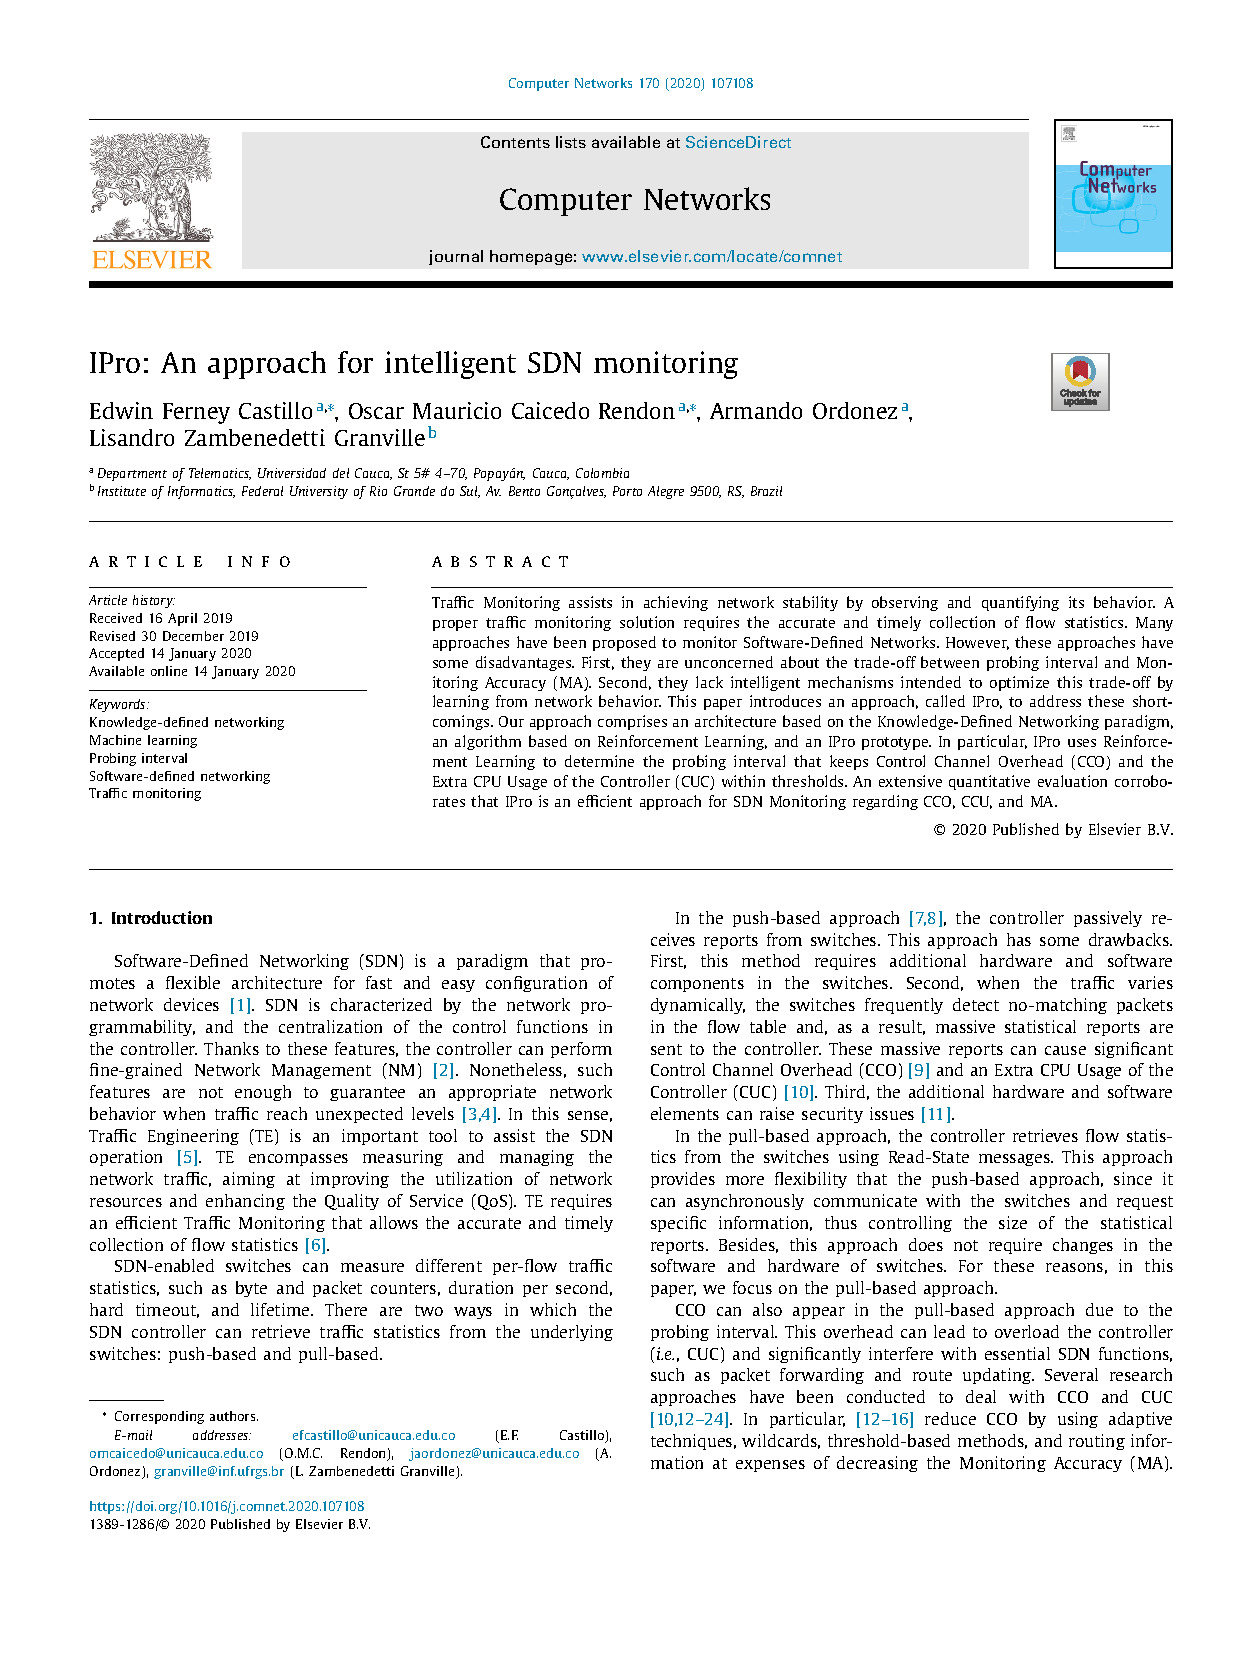
\includepdf[pages=-]{Anexos/IPro_Paper.pdf}
 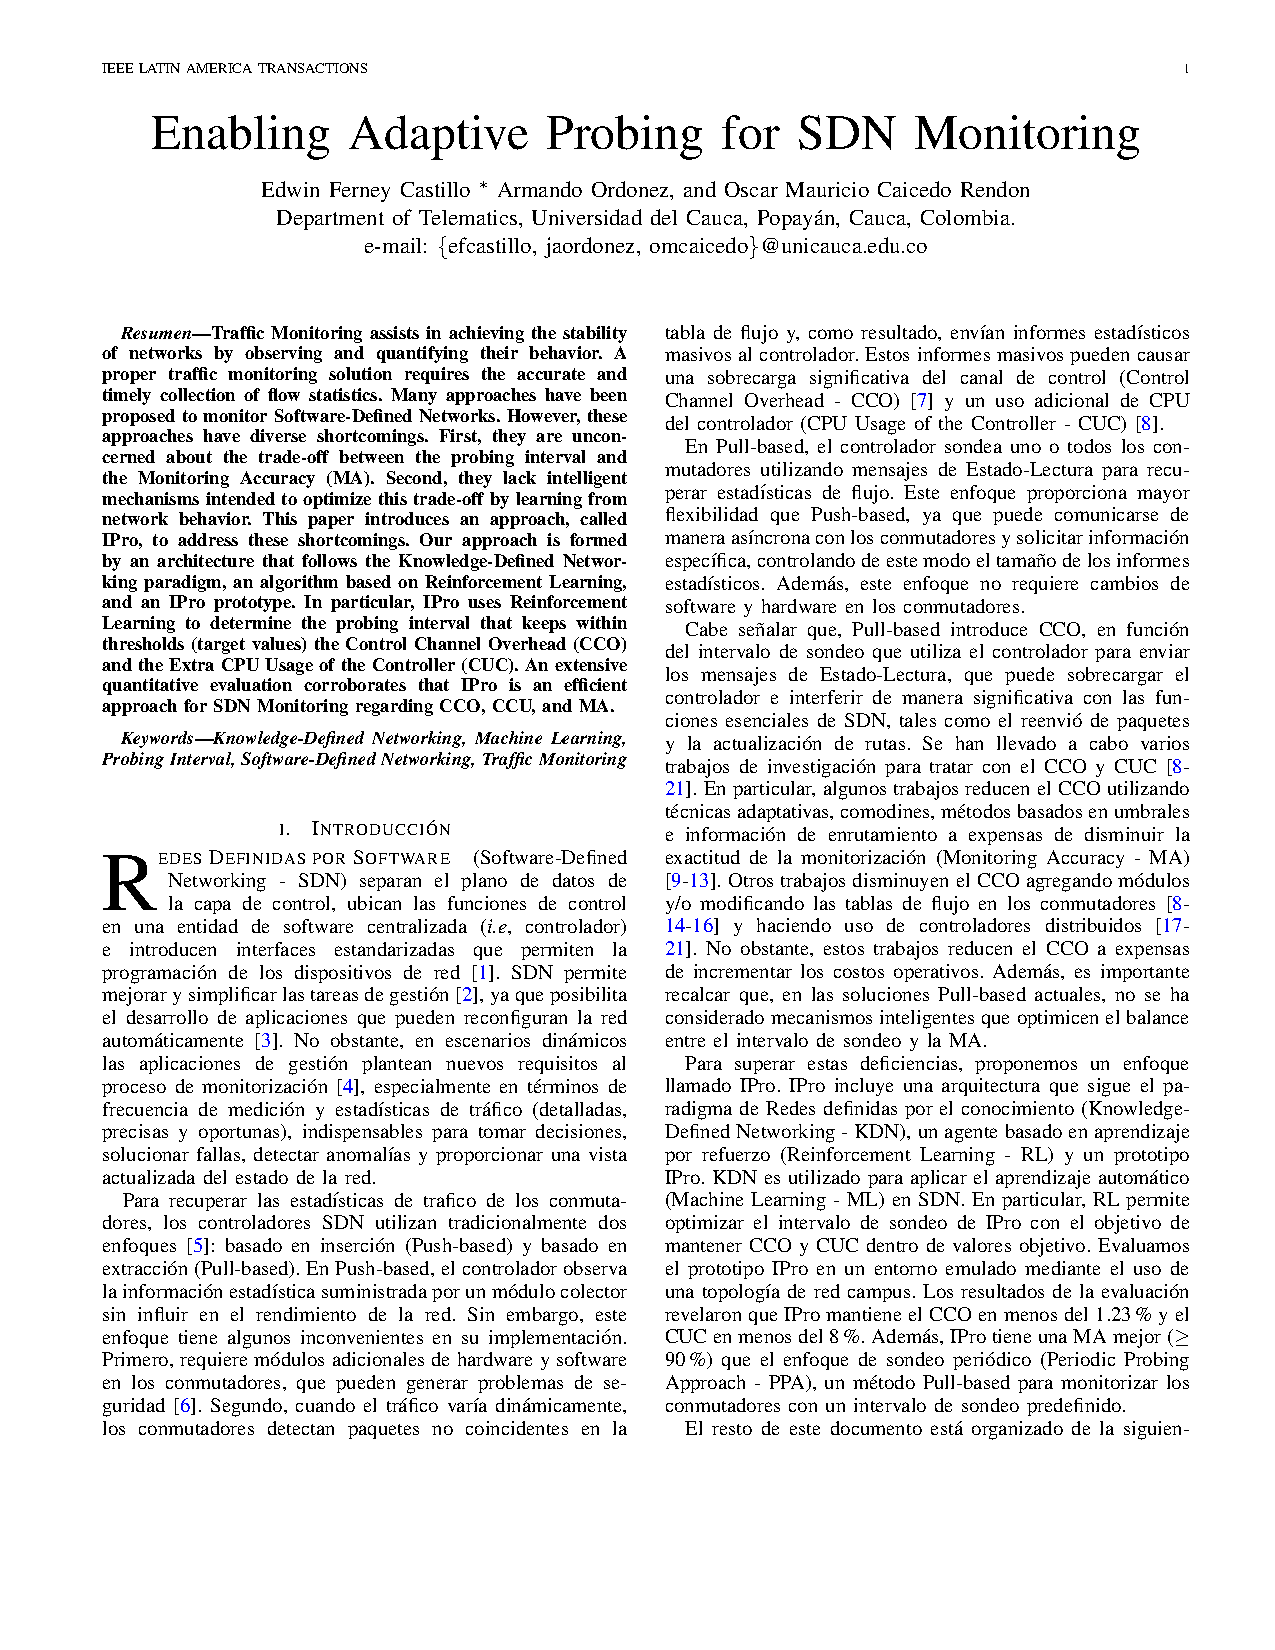
\includepdf[pages=-]{Anexos/IPro_LatinAmericaTransactions.pdf}
\end{document}